\documentclass[twocolumn, a4paper]{article}
\usepackage{graphicx} % Required for inserting images
\usepackage{caption} % Captions
\usepackage{bbm} % Math font; use \mathbbm{}
\usepackage[acronym]{glossaries} % Acronyms
\usepackage[authoryear]{natbib} % Bibliography
\usepackage{physics} % Physics symbols

% \usepackage{showlabels} % To show equations labels on the PDF. Comment at the end

\newacronym{df}{DF}{Distribution Function}
\newacronym{cdf}{CDF}{Chandrasekhar’s dynamical
friction}
\newacronym{nfw}{NFW}{Navarro-Frenk-White}
\newacronym{pdf}{PDF}{probability density function}
\newacronym{krr}{KRR}{kernel ridge regression}

\title{Dynamical Friction and Orbital Evolution in a Modified Navarro-Frenk-White Profile}
\author{Federico Leto di Priolo}
\date{April 2025}

\begin{document}

\maketitle

\begin{abstract}
    The purpose of this work is to study the orbit of a satellite in a dense environment through numerical simulations, with particular focus on the dynamical friction acting on the satellite and the evolution of its orbital eccentricity. We explore a highly simplified scenario in which a point-mass particle moves within a collisionless, isotropic, and spherically symmetric stellar density profile. We find that the \acrlong{cdf} formula provides—despite some caveats—a qualitatively good approximation of the gravitational drag experienced by the satellite. Furthermore, the satellite’s orbit shows a clear tendency toward circularization, regardless of its initial conditions.
\end{abstract}

\section{Introduction}

The main idea is inspired by \citet{Vasiliev2022}, who studied the radialization of satellite orbits in galaxy mergers. The key question is whether a simplified approach to the problem can qualitatively reproduce similar results. The simulations in the original work by \citeauthor{Vasiliev2022} account for several aspects of the system, such as satellite mass loss and host distortion. In contrast, my approach is more straightforward: a point mass moving in a collisionless, isotropic, spherical distribution of point-like particles.

\citeauthor{Vasiliev2022} adopt density profiles that closely resemble pure power laws (\(\rho \propto r^{-\gamma}\)). As a rule of thumb, they observe a general increase in the satellite's eccentricity for the \(\gamma = 1\) and \(\gamma = 2\) cases, while in the \(\gamma = 3\) scenario, there is a tendency toward circularization. Moreover, in their simulations, the prediction from the \acrfull{cdf} formula does not match the observed orbital evolution.

My ultimate goal is to assess whether the \acrshort{cdf} provides a good representation of the instantaneous dissipative force acting on the satellite during its inspiral through the host distribution, and to track the evolution of its orbital eccentricity.

\subsection{Choice of the distribution}

The \acrfull{nfw} profile (Eq.~\ref{eq:rho_NFW}) is a commonly used dark matter distribution in N-body simulations. It can describe a wide range of halo masses and provides a good fit to most rotation curve data. Moreover, it depends on only two parameters and behaves as a \(\gamma = 1\) and \(\gamma = 3\) power law for \(r \ll R_\text{s}\) and \(r \gg R_\text{s}\), respectively. For these reasons, I chose it as the starting point for defining the host distribution.
\begin{equation}
    \rho_\text{NFW}\qty(r) = \dfrac{\rho_0}{\dfrac{r}{R_\text{s}} \qty(1 + \dfrac{r}{R_\text{s}})^2}.
    \label{eq:rho_NFW}
\end{equation}
However, its total integrated mass diverges, requiring an artificial truncation of the distribution. Alternatively, a finite mass can be obtained by applying a smoother cutoff. The natural choice would be an exponential cutoff (e.g., \(\exp(-\qty(r/R_\text{vir}))\)), but I opted for a slightly shallower factor:
\begin{equation}
    \rho\qty(r) = \rho_0 \dfrac{y \csch(y)}{x \qty(1 + x)^2},
    \label{eq:rho}
\end{equation}
where \(x = r / R_\text{s}\), \(y = r / R_\text{vir}\), and \(R_\text{vir} = c R_\text{s}\) is the virial radius, defined via the concentration parameter \(c\). The virial radius is used in the \acrshort{nfw} profile to define the outer boundary of the distribution and its total mass. The value of \(c\) typically ranges from 4 to 40 for halos of different sizes. This choice minimally affects the distribution’s properties at small radii (\(r < R_\text{vir}\)), such as the integrated mass, potential, and circular velocity, which remain close to those of the original \acrshort{nfw} profile.

Figures \ref{fig:density_comp}, \ref{fig:mass_comp}, \ref{fig:v_circ_comp}, and \ref{fig:potential_comp} compare the properties of three profiles — the plain \acrshort{nfw}, the exponentially cut profile, and the hyperbolically cut profile — using a fixed choice of \(\rho_0\), \(R_\text{s}\), and \(c\) (later used in the simulation). In the hyperbolic case, the total mass of the distribution (indicated by the red horizontal line in Fig.~\ref{fig:mass_comp}) is given by:
\begin{equation}
    M_\text{tot} = 4 \pi \rho_0 R_\text{s}^3 \int_0^\infty \qty(\frac{x}{c^{-1} + x})^2 \csch(x) \dd{x}.
    \label{eq:M_tot}
\end{equation}

\begin{figure}
    \centering
    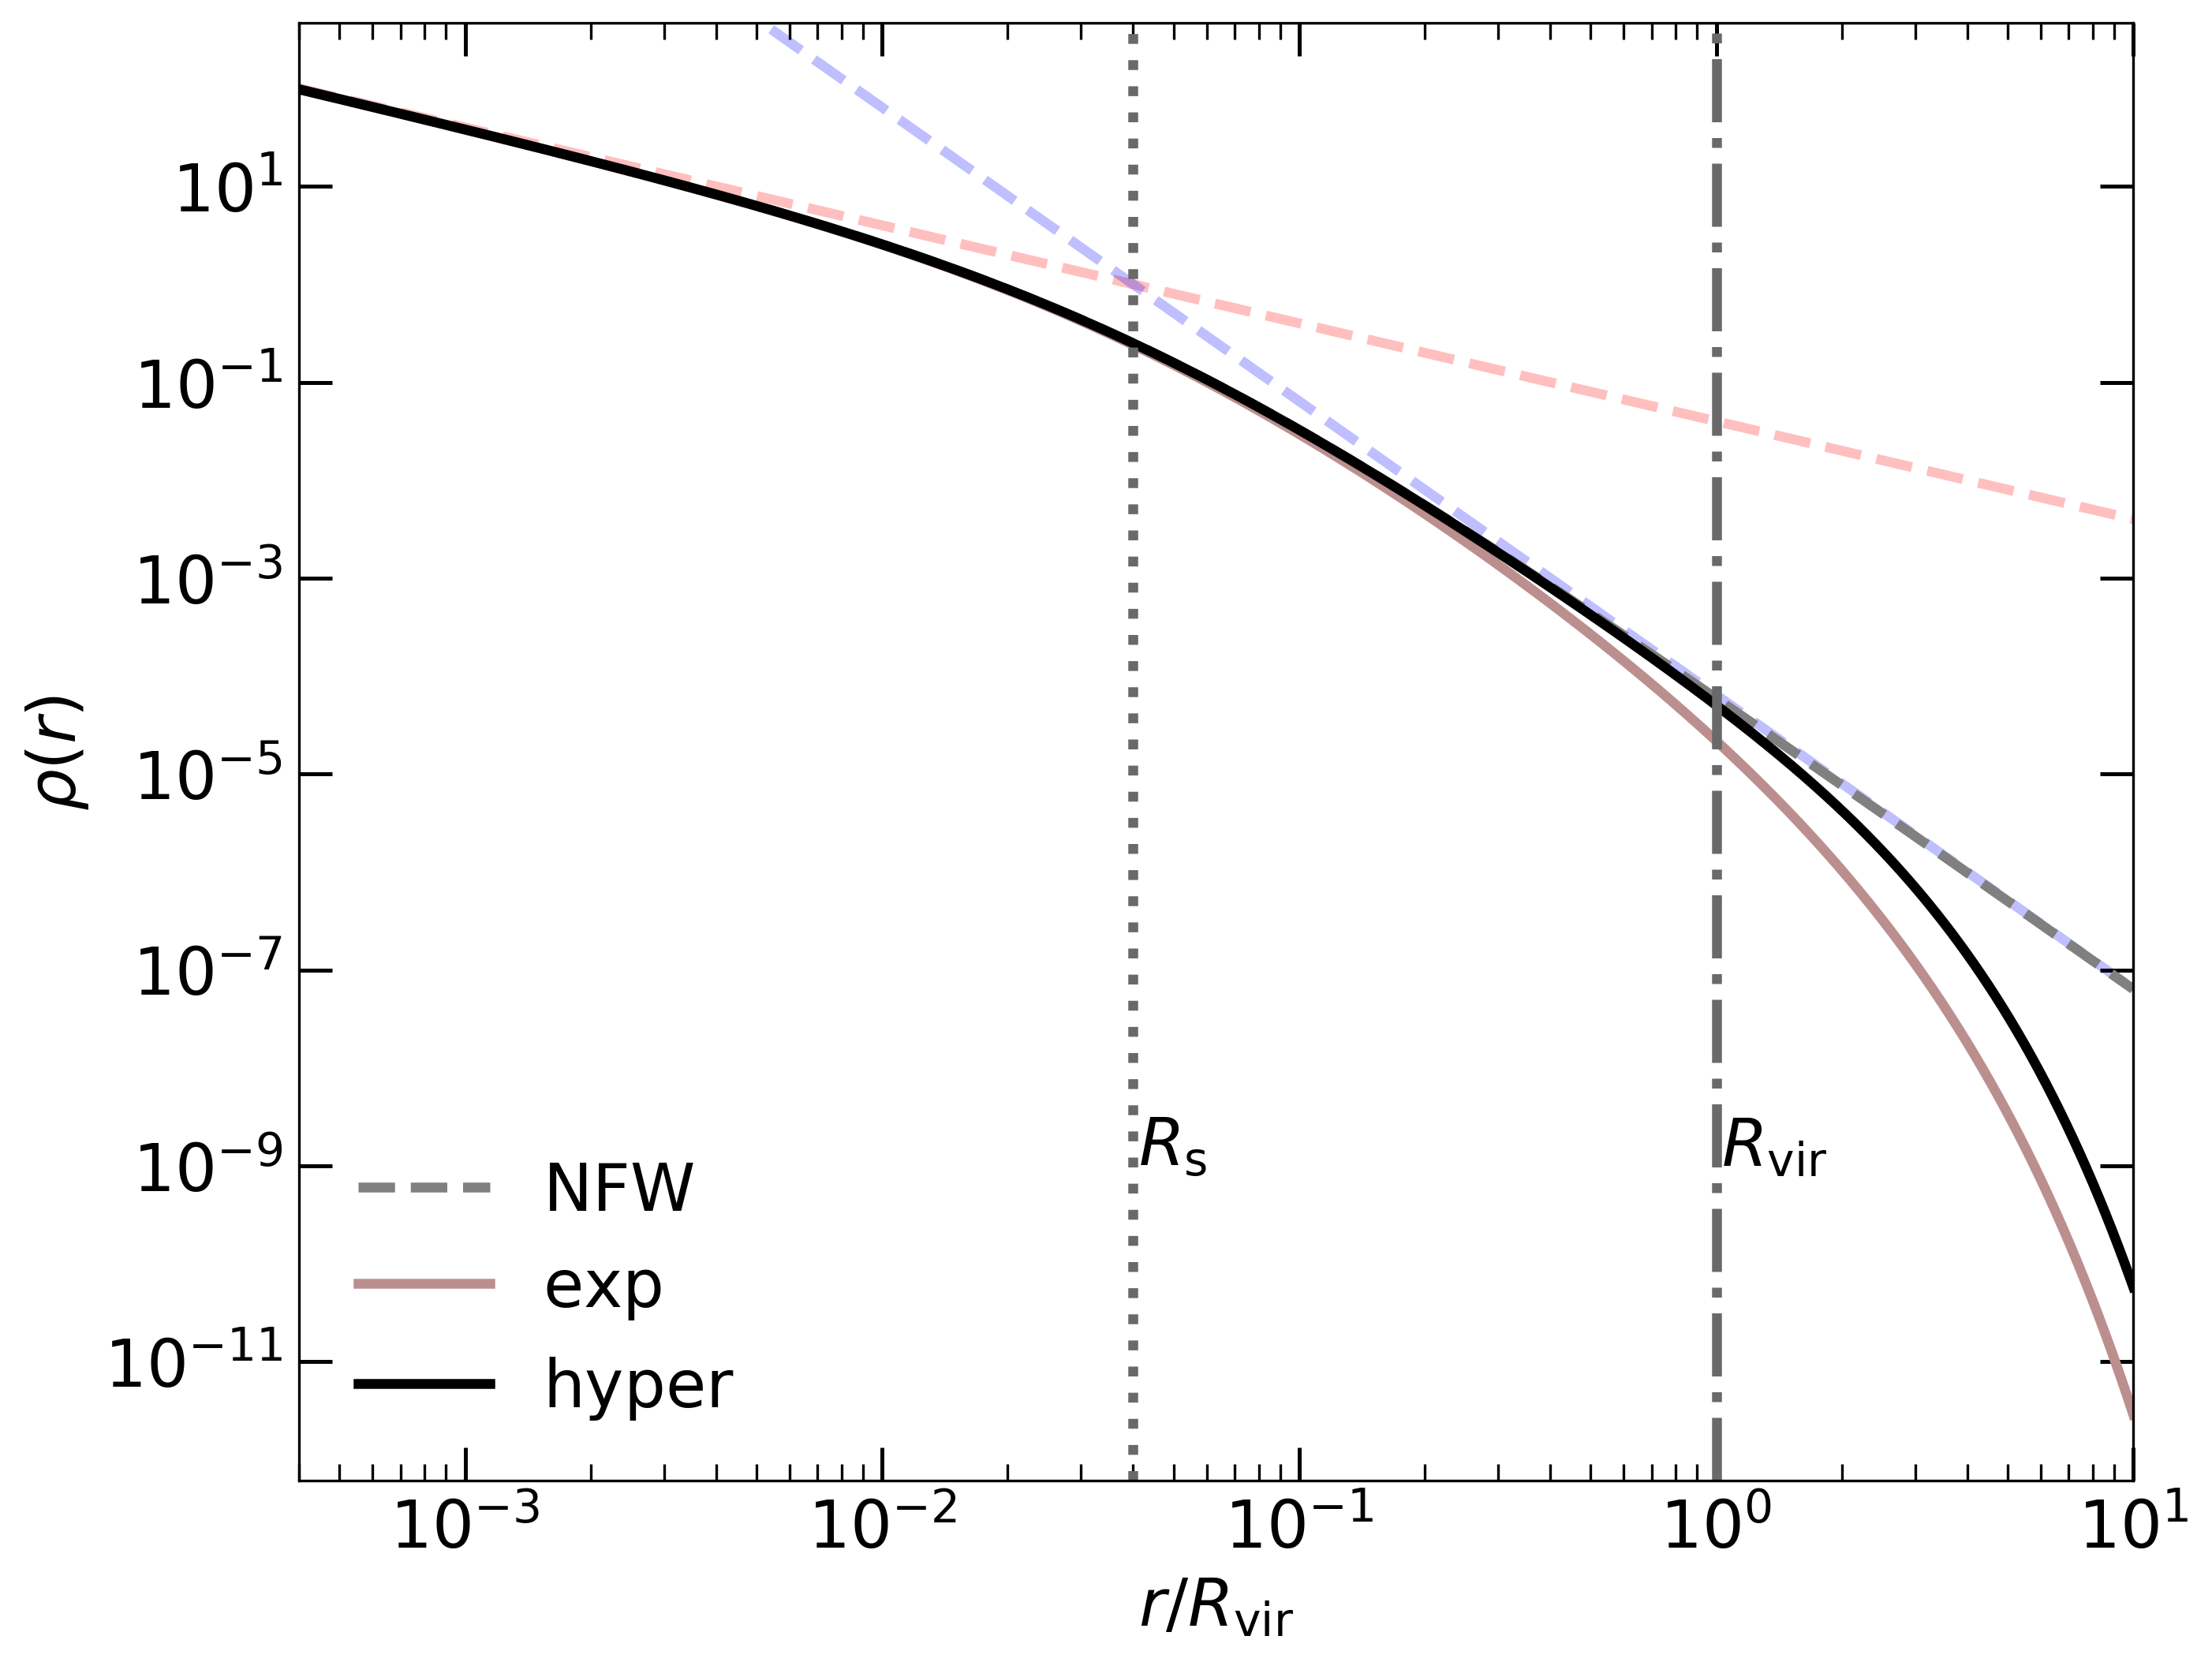
\includegraphics[width=\columnwidth]{images/density_comparison.png}
    \caption{Density profiles. \(\text{NFW}\), '\(\text{exp}\)', and '\(\text{hyper}\)' denote the plain \acrshort{nfw} profile, the exponentially cut profile, and the hyperbolically cut profile, respectively. The dotted and dashed-dotted vertical lines mark the scale radius \(R_\text{s}\) and the virial radius \(R_\text{vir}\). The plot refers to the specific case \(\rho_0 = 1\), \(R_\text{s} = 1\), and \(c = 25\). The red and blue dashed lines indicate constant slopes of \(\gamma = 1\) and \(\gamma = 3\), for reference.}
    \label{fig:density_comp}
\end{figure}

\begin{figure}
    \centering
    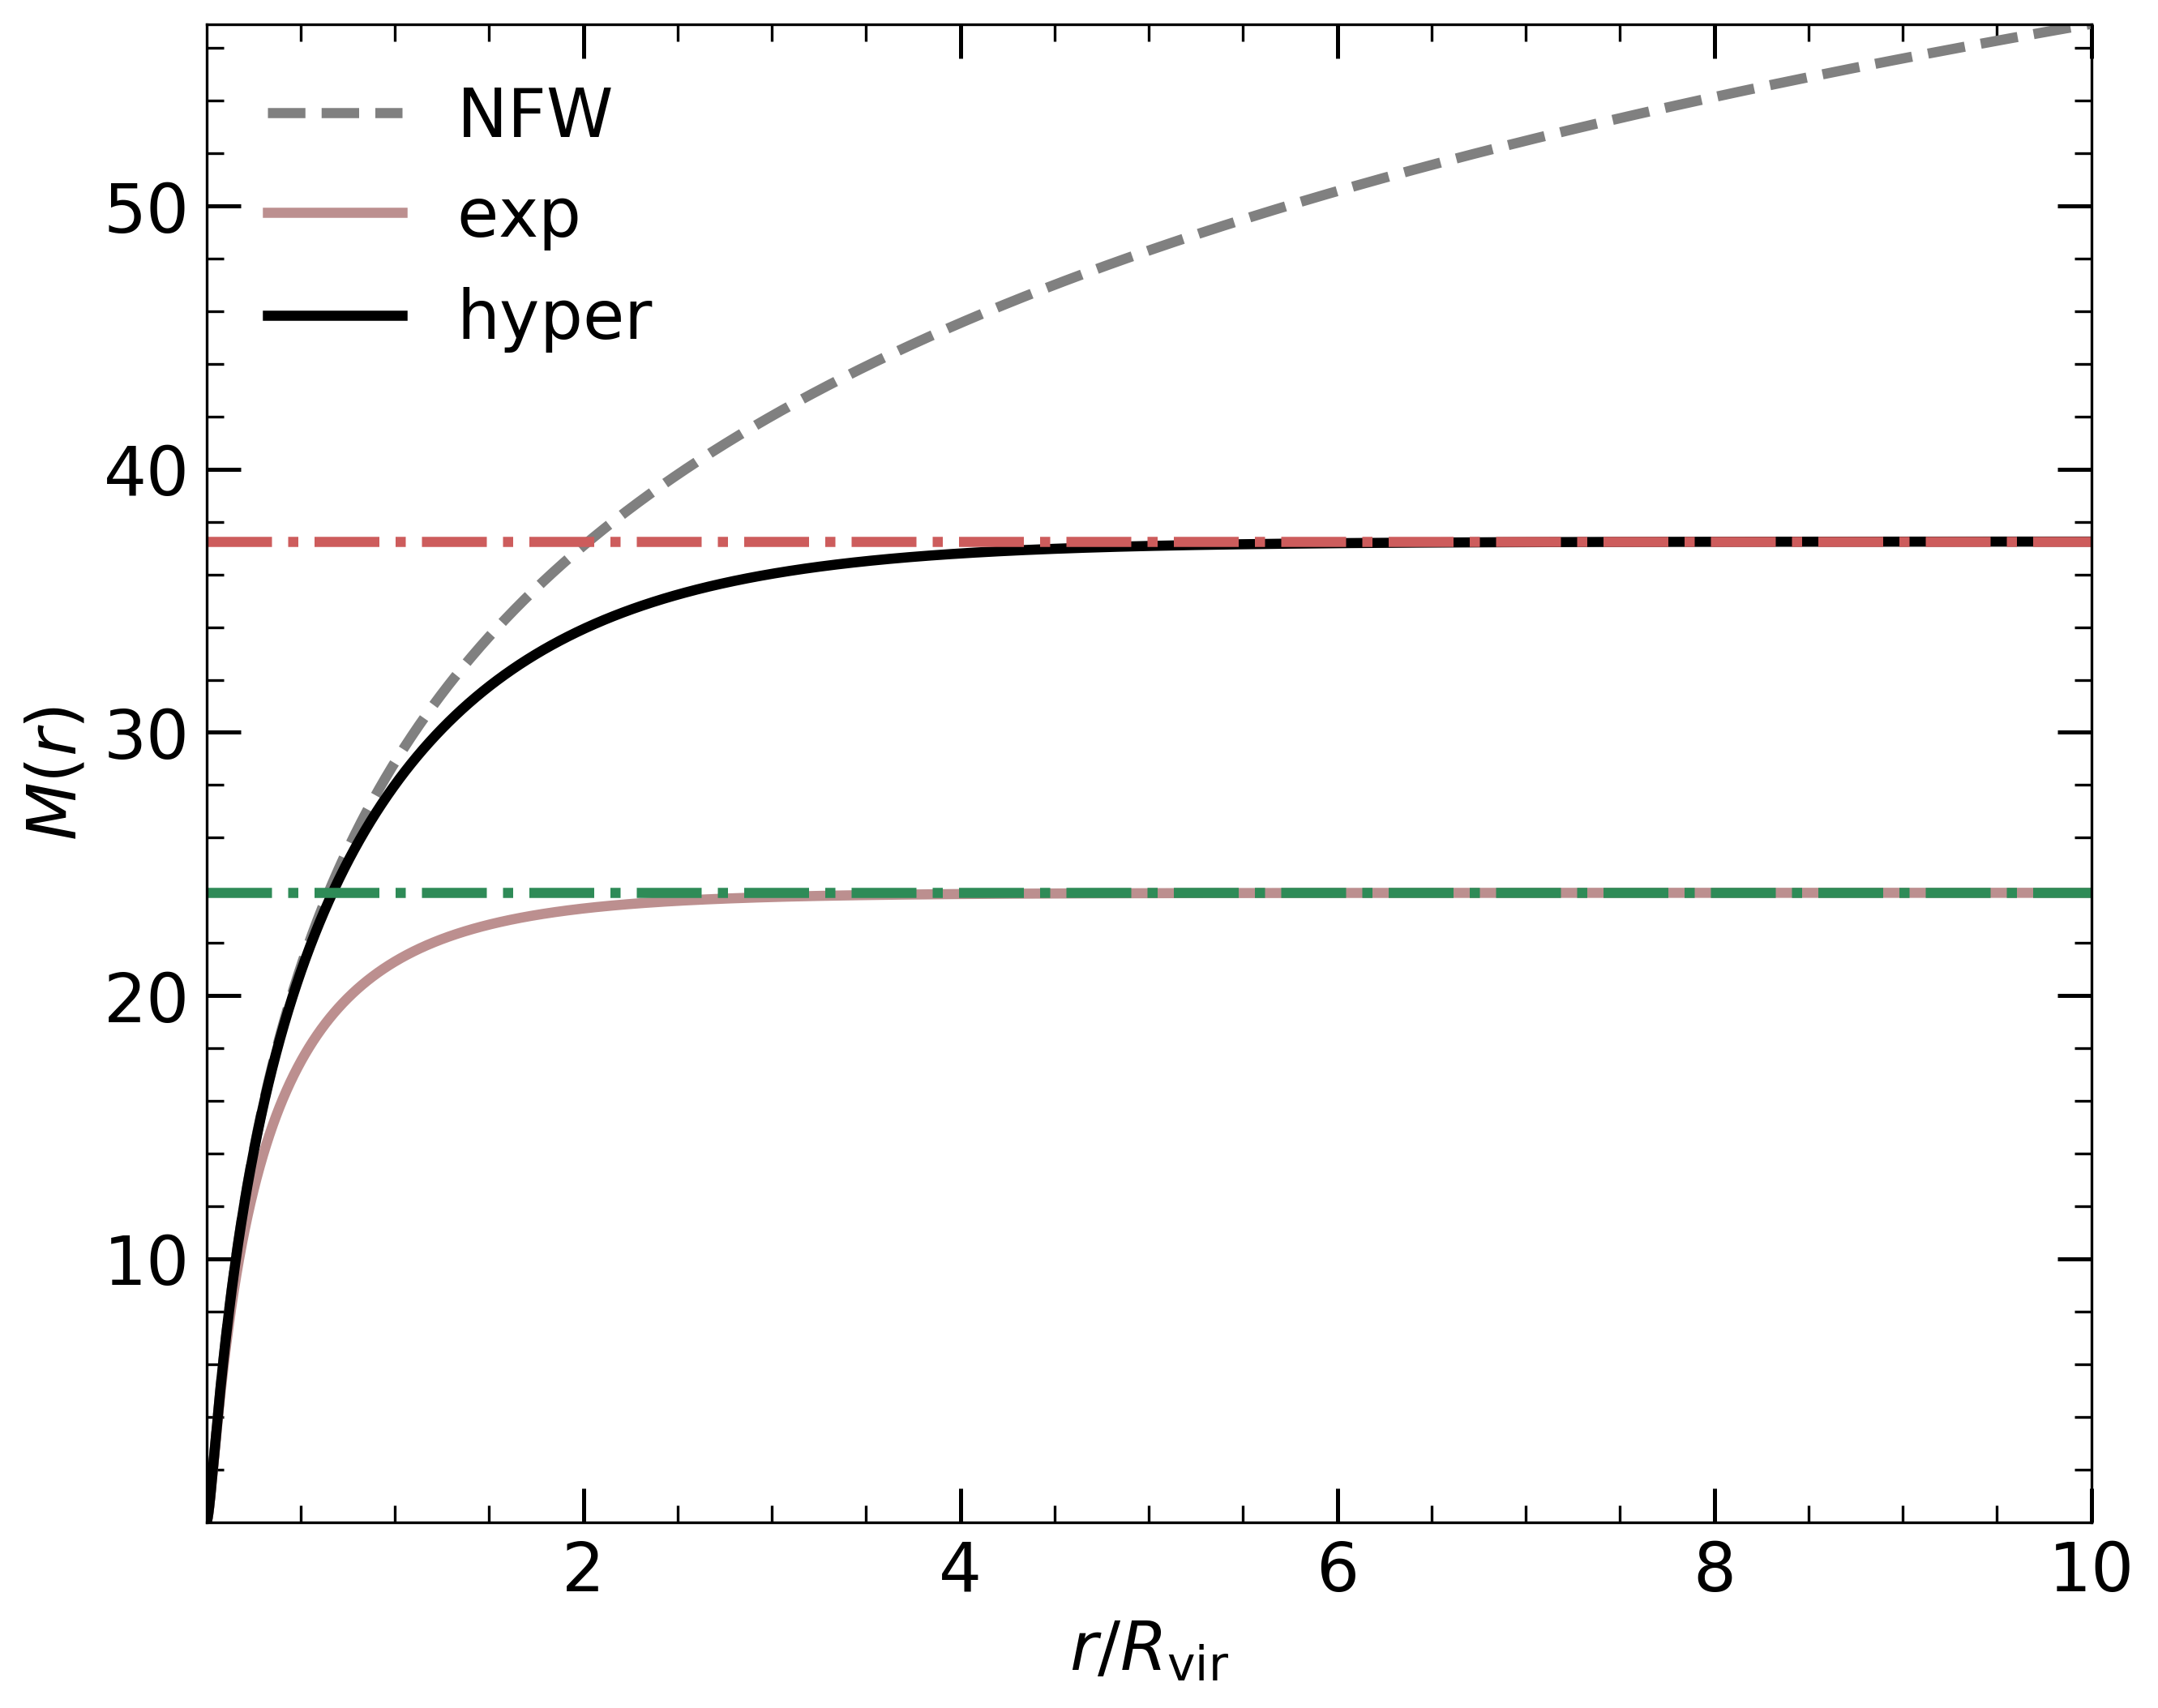
\includegraphics[width=\columnwidth]{images/mass_comparison.png}
    \caption{Integrated mass. Same profiles as in Fig.~\ref{fig:density_comp}. The horizontal dashed-dotted lines mark the total mass for the '\(\text{exp}\)' and '\(\text{hyper}\)' profiles.}
    \label{fig:mass_comp}
\end{figure}

\begin{figure}
    \centering
    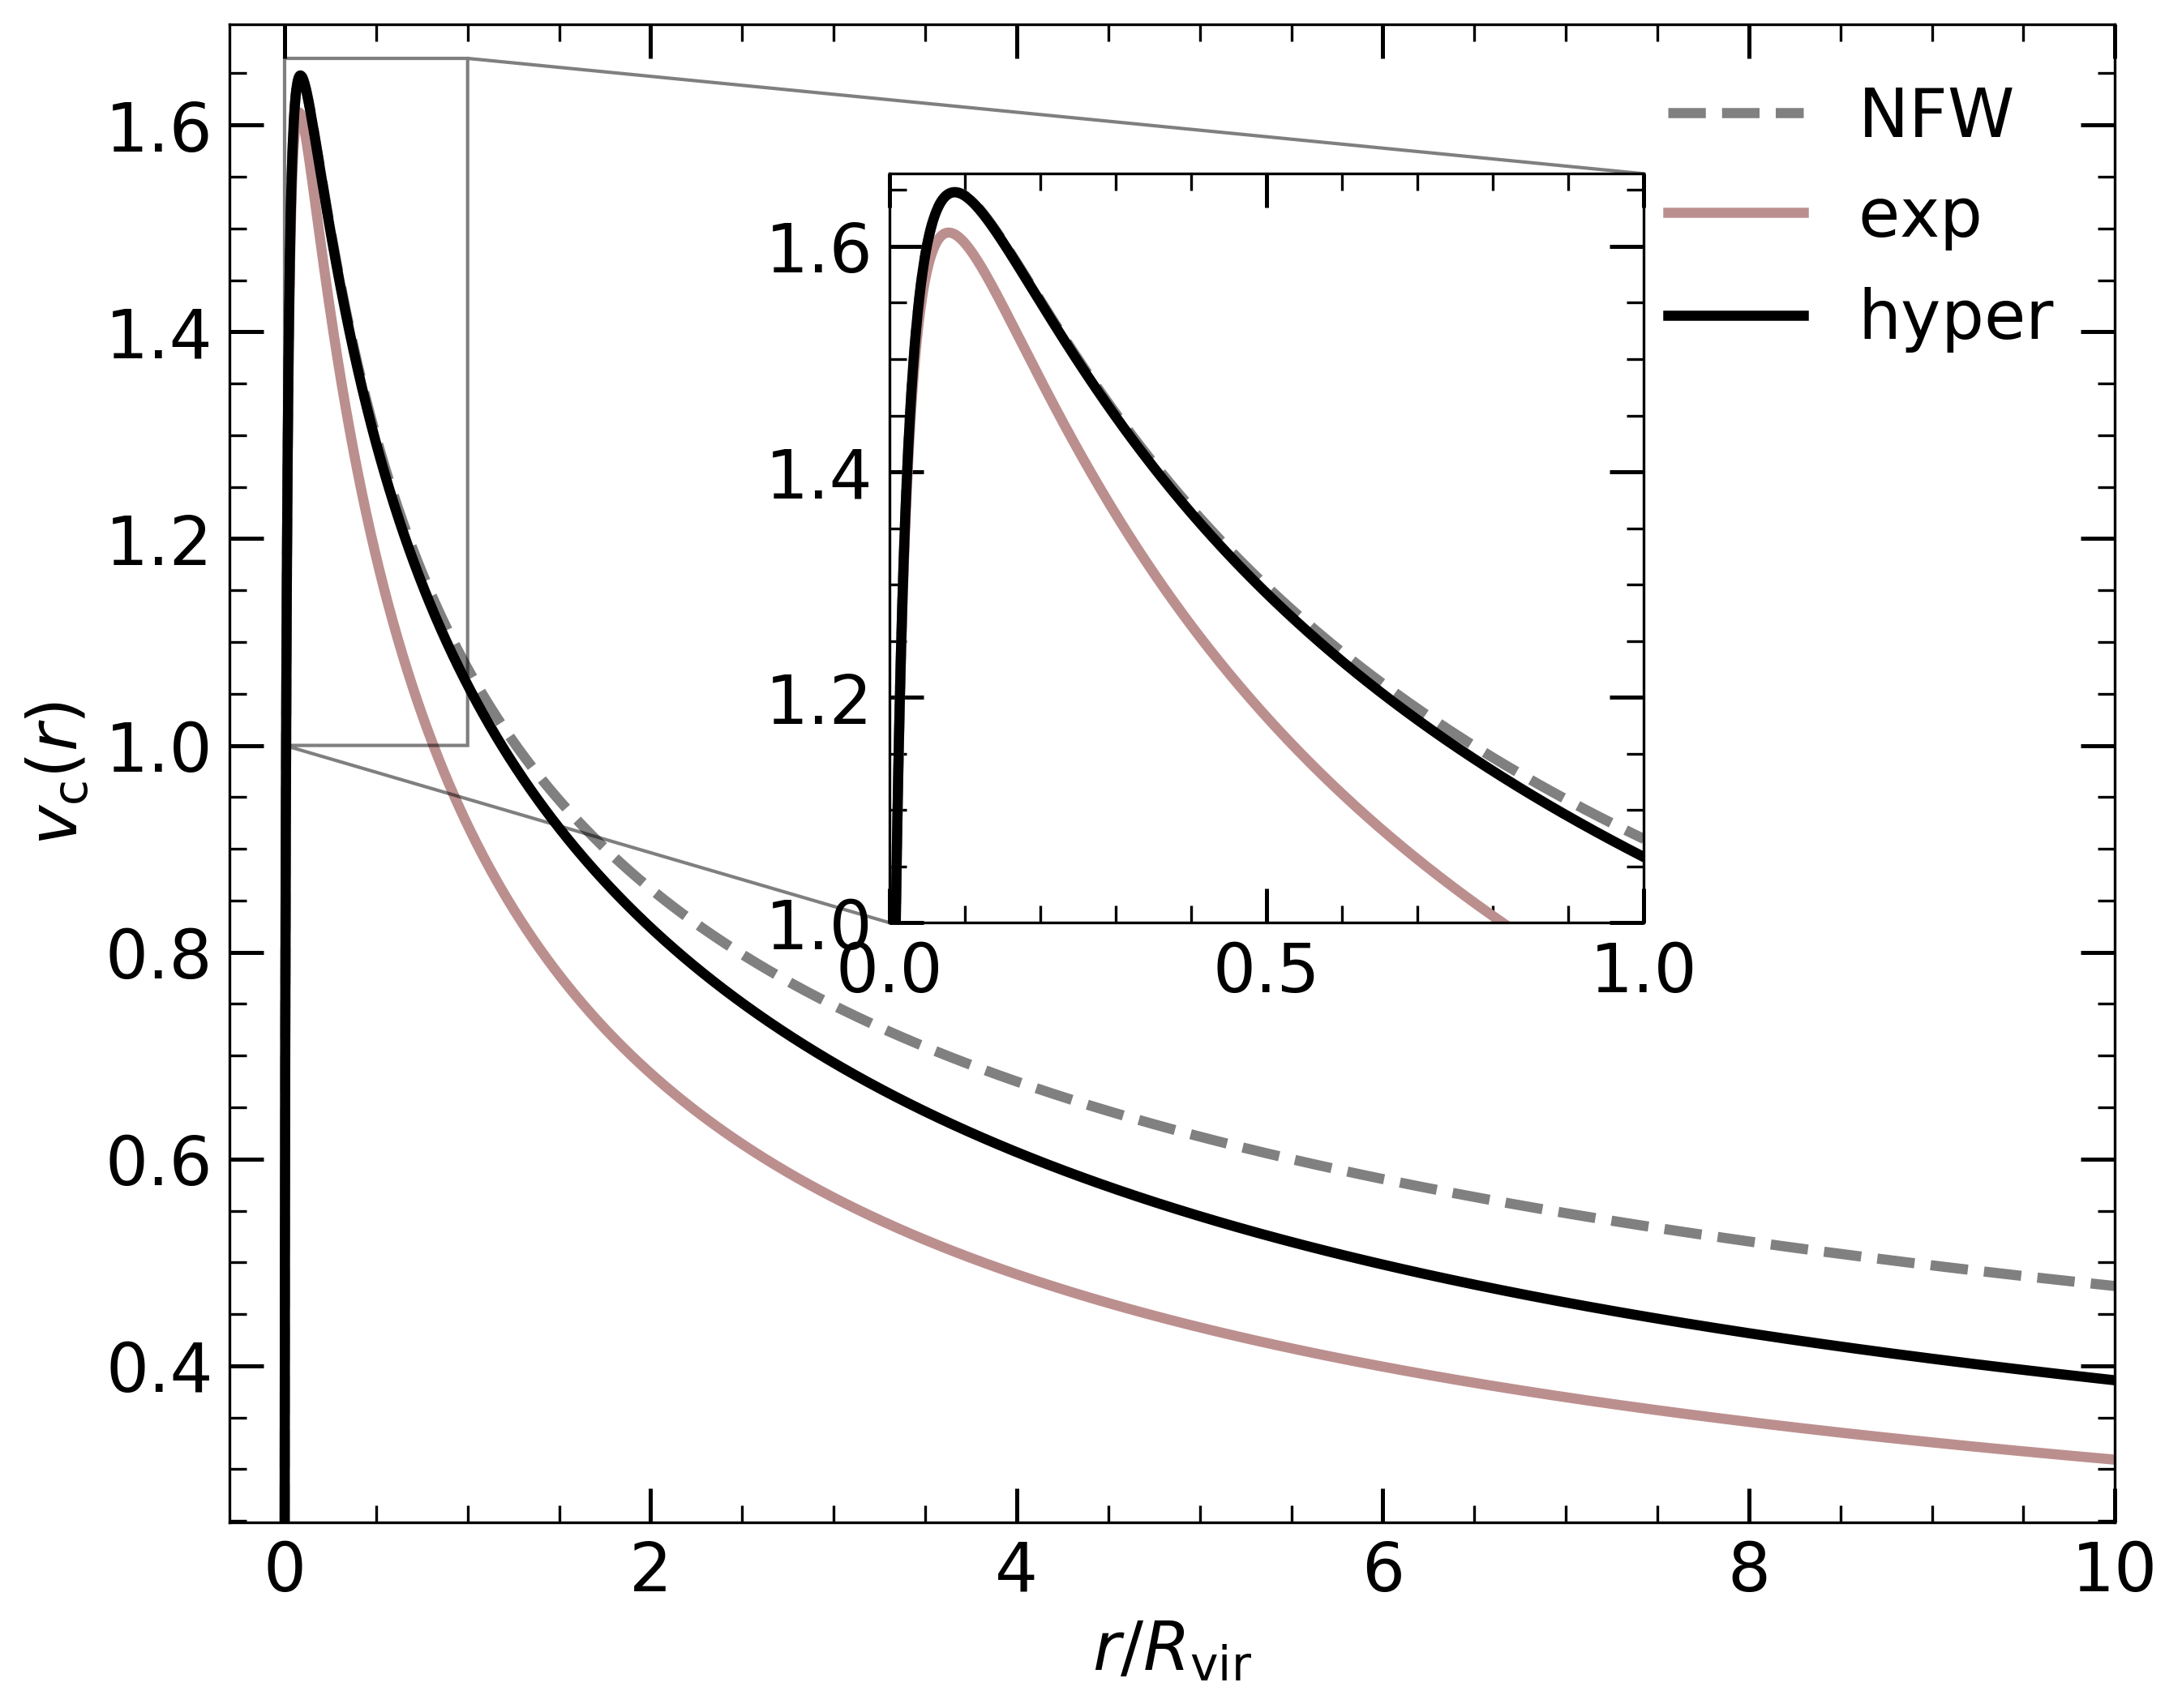
\includegraphics[width=\columnwidth]{images/v_circ_comparison.png}
    \caption{Circular velocity. Same profiles as in Fig.~\ref{fig:density_comp}.}
    \label{fig:v_circ_comp}
\end{figure}

\begin{figure}
    \centering
    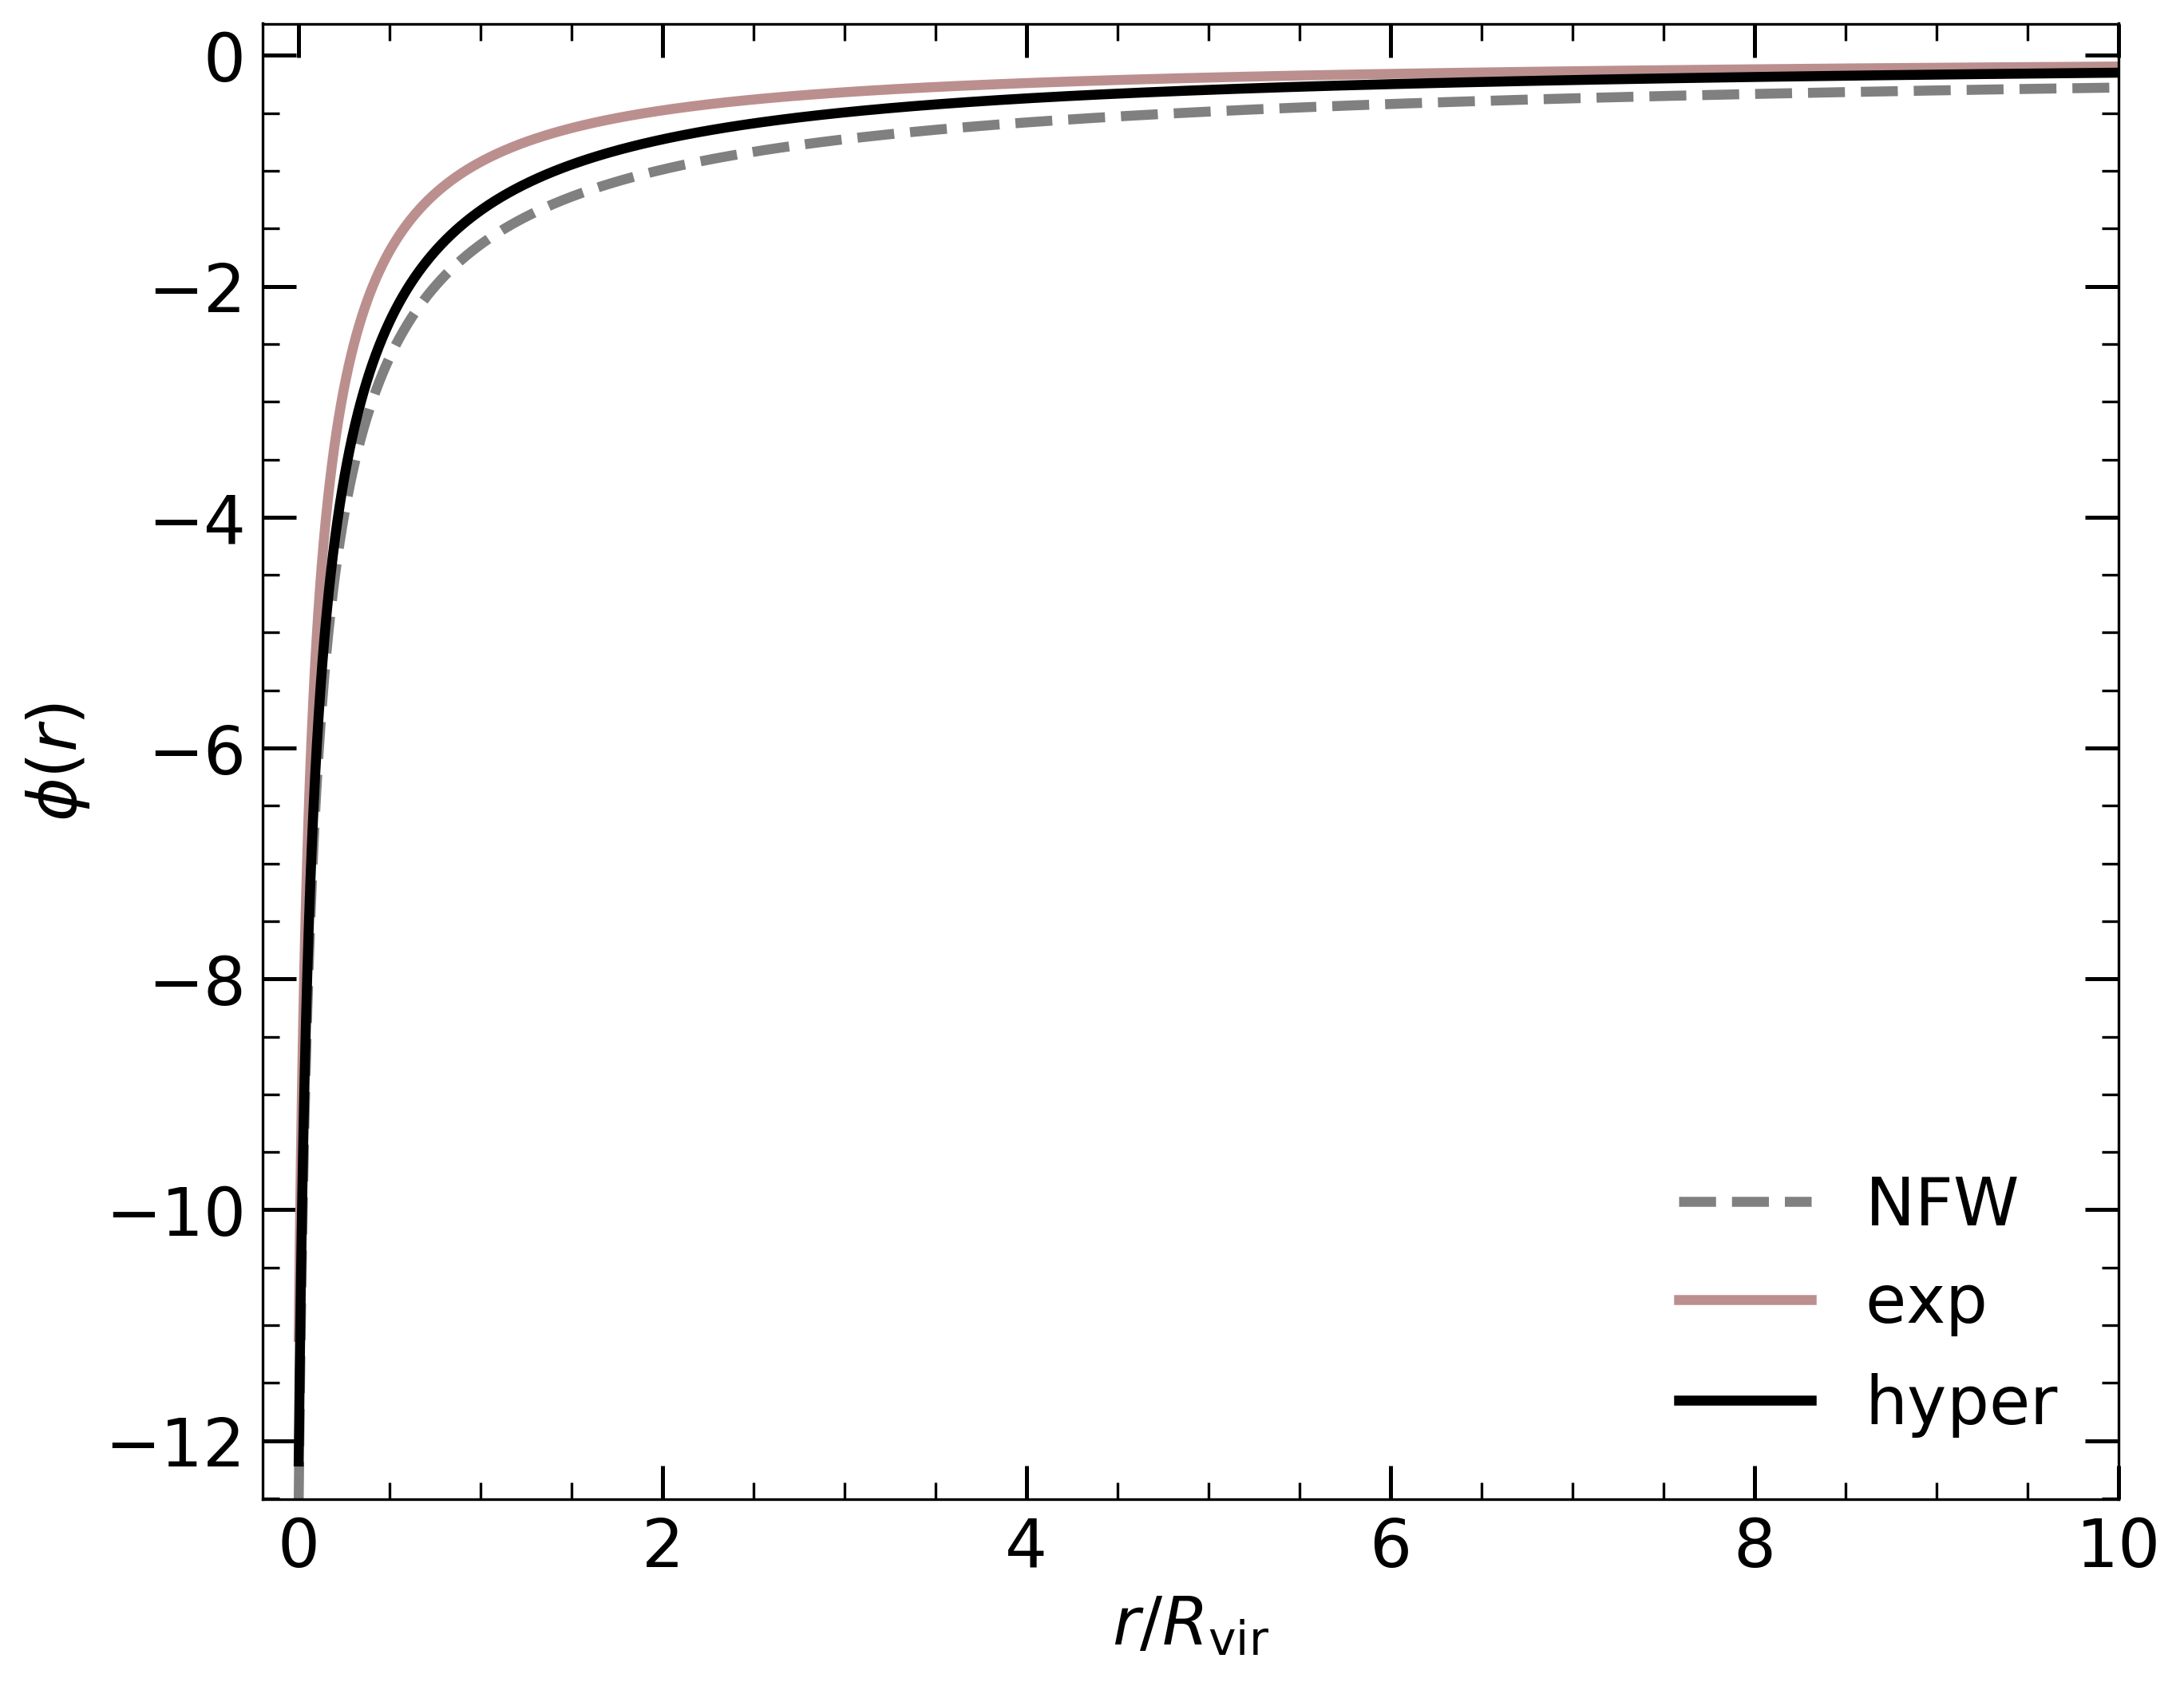
\includegraphics[width=\columnwidth]{images/potential_comparison.png}
    \caption{Potential. Same profiles as in Fig.~\ref{fig:density_comp}.}
    \label{fig:potential_comp}
\end{figure}

\subsection{\acrlong{cdf}} \label{sec:cdf_intro}

Dynamical friction refers to the gravitational drag force experienced by a body (the satellite) moving through a matter distribution (the host). In an isotropic and homogeneous distribution, and under the assumption that the satellite is less massive than the host but more massive than its individual stars, it is possible to derive a first-order approximation of the cumulative effect exerted by the background particles on the moving body — the \acrfull{cdf} formula:
\begin{multline}
    \dv{\vb{v}_M}{t} = -16 \pi^2 G^2 m\qty(M + m) \\
    \ln\Lambda \qty[\int_0^{v_M} \dd{v} v^2 f\qty(v)] \dfrac{\vb{v}_M}{v_M^3}.
    \label{eq:cdf}
\end{multline}
Here, \(M\) and \(\vb{v}_M\) are the mass and velocity of the satellite, \(m\) is the mass of the individual host particles, \(\ln\Lambda\) is the Coulomb logarithm, and \(f(v)\) is the distribution function of the host's stars.

The \acrshort{cdf} formula assumes an infinite and homogeneous medium, but the main source of uncertainty in Eq.~\ref{eq:cdf} is the Coulomb logarithm. Although a fixed value of \(\Lambda\) may provide a good approximation, computing it by accounting for the local properties of the distribution around the perturber — as suggested by \citet{Just2010} — can improve the accuracy of the result.

\section{Methods}

The workflow can be divided into three main steps:
\begin{enumerate}
    \item Generate the distribution defined by the chosen density profile (Eq.~\ref{eq:rho}) in an equilibrium configuration, and initialize a massive perturber within it.
    \item Run a numerical simulation for a sufficiently long time, allowing the perturber's orbit to decay toward the center of the distribution.
    \item Compute the \acrshort{cdf} and track the evolution of the perturber's orbital eccentricity throughout the simulation.
\end{enumerate}

In the preliminary phase, I generate an unperturbed distribution to verify its stability over its characteristic dynamical time scale. Finally, I compare the acceleration of the perturber computed from Eq.~\ref{eq:cdf} with the actual one, and analyze the resulting eccentricity behavior.

\subsection{Generation of the distribution at the equilibrium} \label{sec:equilibrium_dist}

The core technique used to generate the distribution's points is rejection sampling. Since the distribution is isotropic and spherically symmetric, the points can be generated in spherical coordinates, one component at a time. For the particle radii, the (normalized) \acrfull{pdf} is simply given by \(p\qty(r) = 4 \pi r^2 \rho\qty(r) / M_\text{tot}\).

To obtain the \acrshort{pdf} for the velocities such that the system is in equilibrium, we need the \acrfull{df} associated with the chosen density profile. Jeans’ theorem states that in a steady state, the \acrshort{df} may depend only on the integrals of motion. For an isotropic and spherically symmetric system, it can be shown that the \acrshort{df} is a function of energy alone. In this case, it can be obtained using the Eddington inversion formula:
\begin{equation}
    f\qty(E) = \dfrac{1}{\sqrt{8}\pi^2} \dv{E} \int_E^0 \dv{\rho}{\phi} \dfrac{\dd{\phi}}{\sqrt{\phi - E}}
    \label{eq:edd_inv_phi},
\end{equation}
where \(\rho\) is the density profile, \(\phi\) is the potential, and \(E\) is the total energy per unit mass. Since the potential for our distribution is not analytic, it is useful to change variables from \(\phi\) to \(r\), leading to:
\begin{equation}
    f\qty(E) = \dfrac{1}{\sqrt{8}\pi^2} \dv{E} \int_{r(E)}^\infty \dv{\rho}{r} \dfrac{\dd{r}}{\sqrt{\phi(r) - E}}
    \label{eq:edd_inv_r},
\end{equation}
where \(r\qty(E)\) is the radius at which \(\phi = E\). Although the solution is guaranteed to be unique, it is not necessarily physical: there may be values of \(E\) for which \(f\qty(E) < 0\). In such cases, a more general \acrshort{df} is required (e.g., \(f\qty(E, L)\)).

Once the \acrshort{df} is obtained, the (non-normalized) velocity \acrshort{pdf} at a fixed position \(R\) can be written as \(p\qty(v, R) = 4 \pi v^2 f\qty(E)\), where \(E = v^2/2 + \phi\qty(R)\). This implies that the radial component of the particles' velocities cannot be sampled independently of their positions, but instead requires prior knowledge of their distance from the center of the distribution.

Finally, the mass of each individual particle is set by \(m = M_\text{tot} / N\), where \(N\) is the total number of particles.

\subsection{Running the simulation}

To estimate the time required for dynamical friction to drag the perturber to the center of the distribution, we can use the following expression:
\begin{equation}
    t_\text{fric} = \dfrac{1.17}{\ln\Lambda} \dfrac{r_i^2 v_c}{G M},
    \label{eq:t_fric}
\end{equation}
from \citet[8.1.1.a]{Binney2011}. Here, \(M\) is the mass of the perturber, \(r_i\) is its initial distance from the distribution center, \(v_c\) is the corresponding circular velocity, and the Coulomb logarithm is fixed to \(\ln\Lambda = 3\). Although Eq.~\ref{eq:t_fric} is derived for a circular orbit in a singular isothermal sphere, it provides a reasonable approximation for other mass distributions as well. The value of \(t_\text{fric}\) obtained in this way is used to appropriately set the stopping time of the numerical simulation.

The smoothing length \(\epsilon\) for the treecode is set to a fraction of the average particle separation in the distribution:
\begin{equation}
    \epsilon = \kappa \dfrac{R_\text{vir}}{N^{1/3}},
    \label{eq:smooth_length}
\end{equation}
where \(0 < \kappa \leq 1\), and \(N\) is the total number of particles. In this case, \(\kappa = 0.1\). Finally, the integration time step \(t_\text{step}\) is defined as:
\begin{equation}
    t_\text{step} = \dfrac{\epsilon}{\sqrt{-2 \phi\qty(\epsilon)}},
    \label{eq:t_step}
\end{equation}
where \(\sqrt{-2 \phi\qty(\epsilon)}\) is the escape velocity from a distance \(\epsilon\) from the center of the distribution.

\subsection{Computation of the \acrshort{cdf} and the orbits' circularity} \label{sec:cdf_circularity_comp}

To compute the integral in Eq.~\ref{eq:cdf}, we need the \acrshort{df} of the field stars at each snapshot of the simulation. After verifying that the distribution remains stable over the timescale of the simulation, we can replace the instantaneous distribution with the one previously obtained using Eq.~\ref{eq:edd_inv_r}. Operationally, at each snapshot, we require the velocity and position of the perturber relative to the center of the distribution. We can then compute \(\int_0^{v_M} \dd{v} \, v^2 f\qty(v^2/2 + \phi\qty(R))\). However, since in our case the \acrshort{df} is derived from the Eddington inversion formula (which is based on the matter density \(\rho\qty(r)\)), we need to recover the correct physical dimension of the acceleration by dividing the result from Eq.~\ref{eq:cdf} by the mass of the field stars, \(m\).

As discussed in Section~\ref{sec:cdf_intro}, to improve the accuracy of the calculation, the Coulomb logarithm is treated as a time-dependent quantity, computed at each snapshot based on the local properties of the distribution around the perturber. Given \(\Lambda = \dfrac{b_\text{max}}{b_\text{min}}\), we require operational definitions for \(b_\text{max}\) and \(b_\text{min}\). At each snapshot, we define \(b_\text{max} = r_p\) and
\[
b_\text{min} = \max\qty(\dfrac{G \qty(M + m)}{v_M^2}, \epsilon) \cdot \dfrac{r_p}{R_\text{vir}},
\]
where \(r_p\) is the distance of the perturber from the center of the distribution and \(\epsilon\) is the smoothing length. The factor \(\dfrac{r_p}{R_\text{vir}}\) in \(b_\text{min}\) accounts for the increasing strength of interactions near the center of the distribution. Since typically \(\dfrac{G \qty(M + m)}{v_M^2} > \epsilon\), for most snapshots we have
\[
\Lambda = \dfrac{v_M^2 R_\text{vir}}{G \qty(M + m)}.
\]

To evaluate the eccentricity of the perturber's orbit at each snapshot, we adopt a simpler approach by computing its circularity. Following \citeauthor{Vasiliev2022}, we define the circularity as \(\eta = L / L_\text{circ}\qty(E)\), i.e., the instantaneous angular momentum of the perturber relative to the host center, normalized by the angular momentum of a circular orbit with the same energy. To compute \(L_\text{circ}\qty(E)\), we need the potential of the distribution at each snapshot. However, as with the \acrshort{df}, it is reasonable to use the (numerically computed) potential derived from the density profile.

Recalling that the effective potential is:
\begin{equation}
    \phi_\text{eff}\qty(r) = \phi\qty(r) + \dfrac{L^2}{2r^2},
    \label{eq:phi_eff}
\end{equation}
and that for a circular orbit \(\dv{\phi_\text{eff}}{r} = 0\), we obtain:
\begin{equation}
    L^2 = r^3 \dv{\phi}{r}.
    \label{eq:l_circ}
\end{equation}
Using Eqs.~\ref{eq:phi_eff} and \ref{eq:l_circ}, we derive the energy of the circular orbit as:
\begin{equation}
    E = \phi\qty(r) + \dfrac{r}{2} \dv{\phi}{r}.
    \label{eq:r_circ}
\end{equation}
Therefore, for a fixed value of \(E\), \(L_\text{circ}\qty(E)\) is given by Eq.~\ref{eq:l_circ} evaluated at the solution of Eq.~\ref{eq:r_circ}.

All quantities mentioned above are measured in the reference frame of the center of the distribution, which is reasonably approximated by the center of mass of the system.

\section{Results}

We now present the results from different simulations in terms of plots and relevant quantities for the analysis of dynamical friction and circularity. Each simulation begins with a matter distribution generated from the density profile (black solid line) shown in Fig.~\ref{fig:density_comp}, using a total of \(N = 10^4\) particles.

The typical timescale of the system is defined as the period of a circular orbit at the virial radius from the center of the distribution:
\begin{equation}
    t_\text{dyn} = 2\pi \sqrt{\dfrac{R_\text{vir}^3}{G M\qty(R_\text{vir})}},
    \label{eq:t_dyn}
\end{equation}
where \(M\qty(R_\text{vir})\) is the mass enclosed within the virial radius. For our distribution, in internal units (\(G = 1\)), this gives \(t_\text{dyn} = 1.484 \times 10^2\). This value is used as the natural time unit for the simulations.

\subsection{\acrlong{df} and \acrlong{pdf}s}

Here we present the resulting \acrshort{pdf}s and the \acrshort{df} obtained through the procedure described in Section~\ref{sec:equilibrium_dist}. Figures~\ref{fig:pdf_r} and \ref{fig:pdf_v} show the \acrshort{pdf} of radii and velocities, respectively, while Figure~\ref{fig:df} displays the \acrshort{df}. In practice, evaluating the Eddington inversion formula to compute the \acrshort{df} can be time-consuming, especially when multiple integrals are required to compute the \acrshort{cdf}. From a technical standpoint, a practical workaround is to fit a model to the computed \acrshort{df} and use it as a surrogate for the exact expression. In this work, I employed the implementation of \acrfull{krr} provided by the scikit-learn library. Using a Laplacian kernel with low regularization allows the model to closely fit the \acrshort{df} values. The fitted model can then be evaluated at any energy value within the original domain.

For this reason, the original \acrshort{df} was computed over the energy range \(\qty[\sim \phi\qty(0), \phi\qty(10 R_\text{vir})]\), which is sufficiently broad for our purposes.

We can assess the validity of the final result by checking whether the fitted \acrshort{df} can reproduce the original density profile. Indeed, the \acrshort{df} must satisfy:
\begin{equation}
    \rho\qty(r) = \int_0^{v_\text{esc}\qty(r)} 4\pi v^2 f\qty(v^2/2 + \phi\qty(r)) \dd{v},
    \label{eq:rho_df}
\end{equation}
where \(v_\text{esc}\qty(r) = \sqrt{-2 \phi\qty(r)}\) is the escape velocity from radius \(r\). The comparison between the original density profile and the one reconstructed from the \acrshort{df} is shown in Figure~\ref{fig:rho_df}.

\begin{figure}
    \centering
    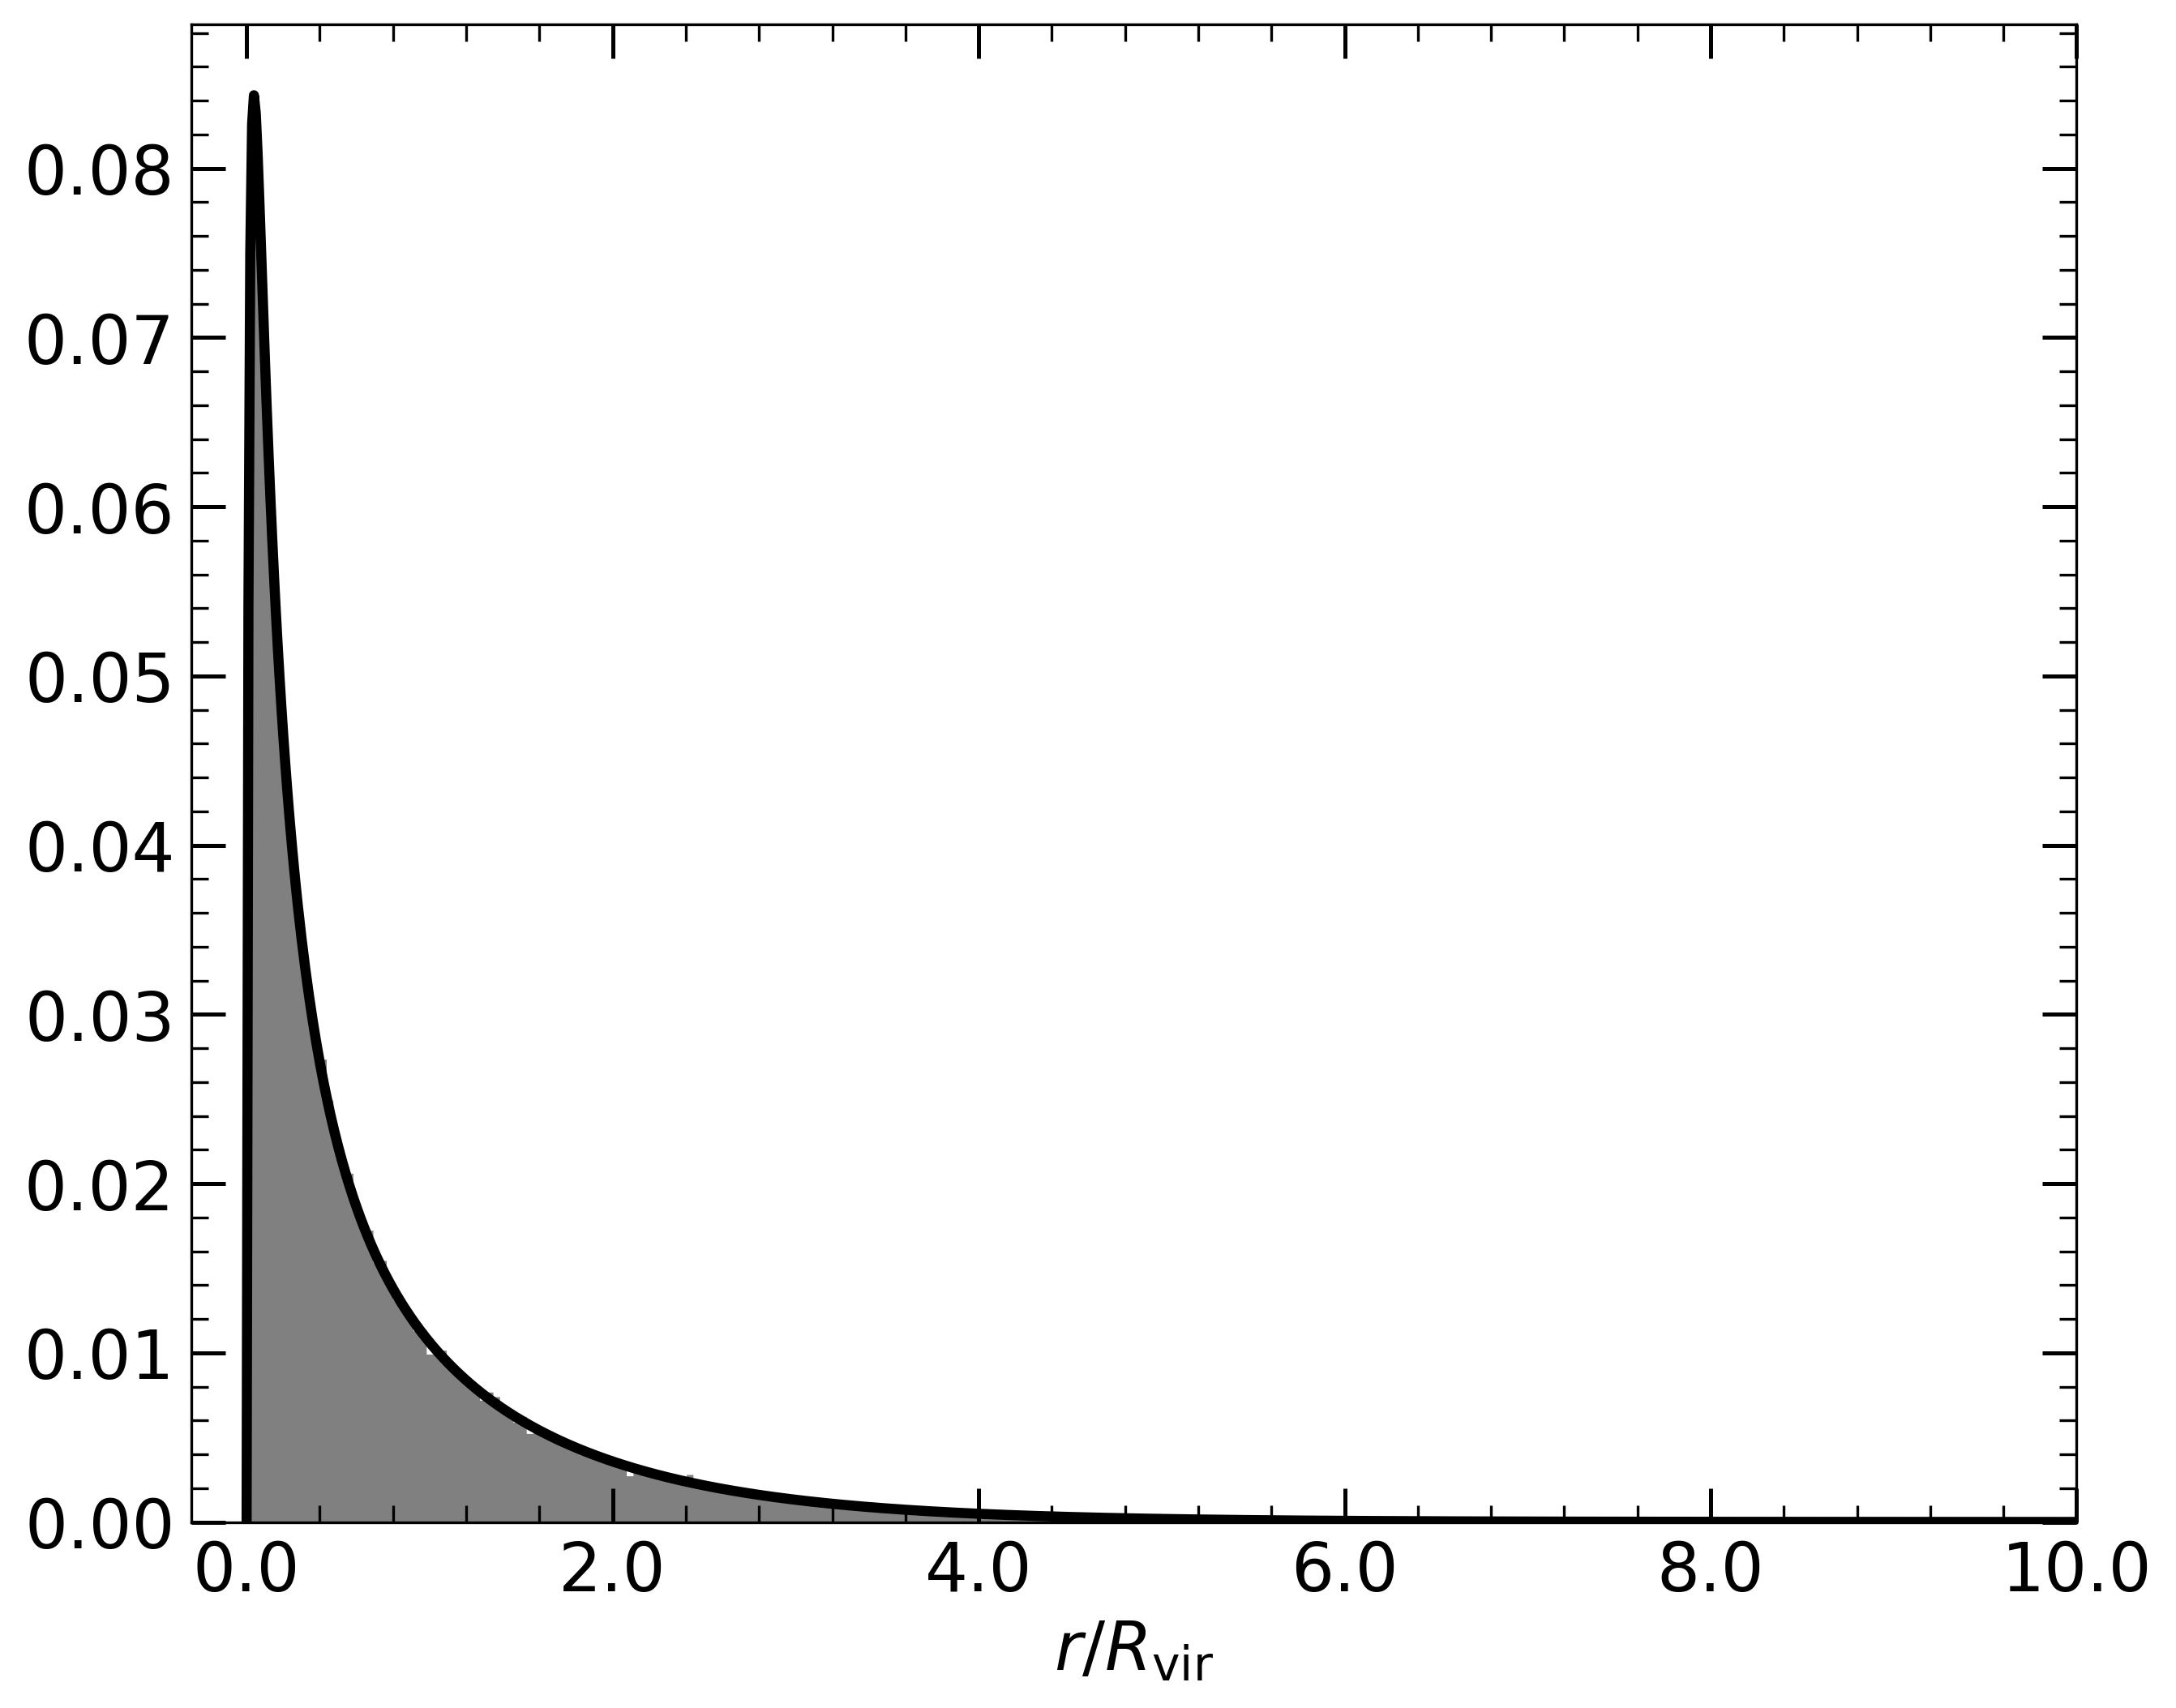
\includegraphics[width=\columnwidth]{images/pdf_r.png}
    \caption{Radial \acrshort{pdf}. The black solid line is the computed \acrshort{pdf}, and the gray shaded area shows an example outcome of the rejection sampling procedure. In both this example and the actual simulations, rejection sampling is performed in the interval \(\qty[0, 10 R_\text{vir}]\).}
    \label{fig:pdf_r}
\end{figure}

\begin{figure}
    \centering
    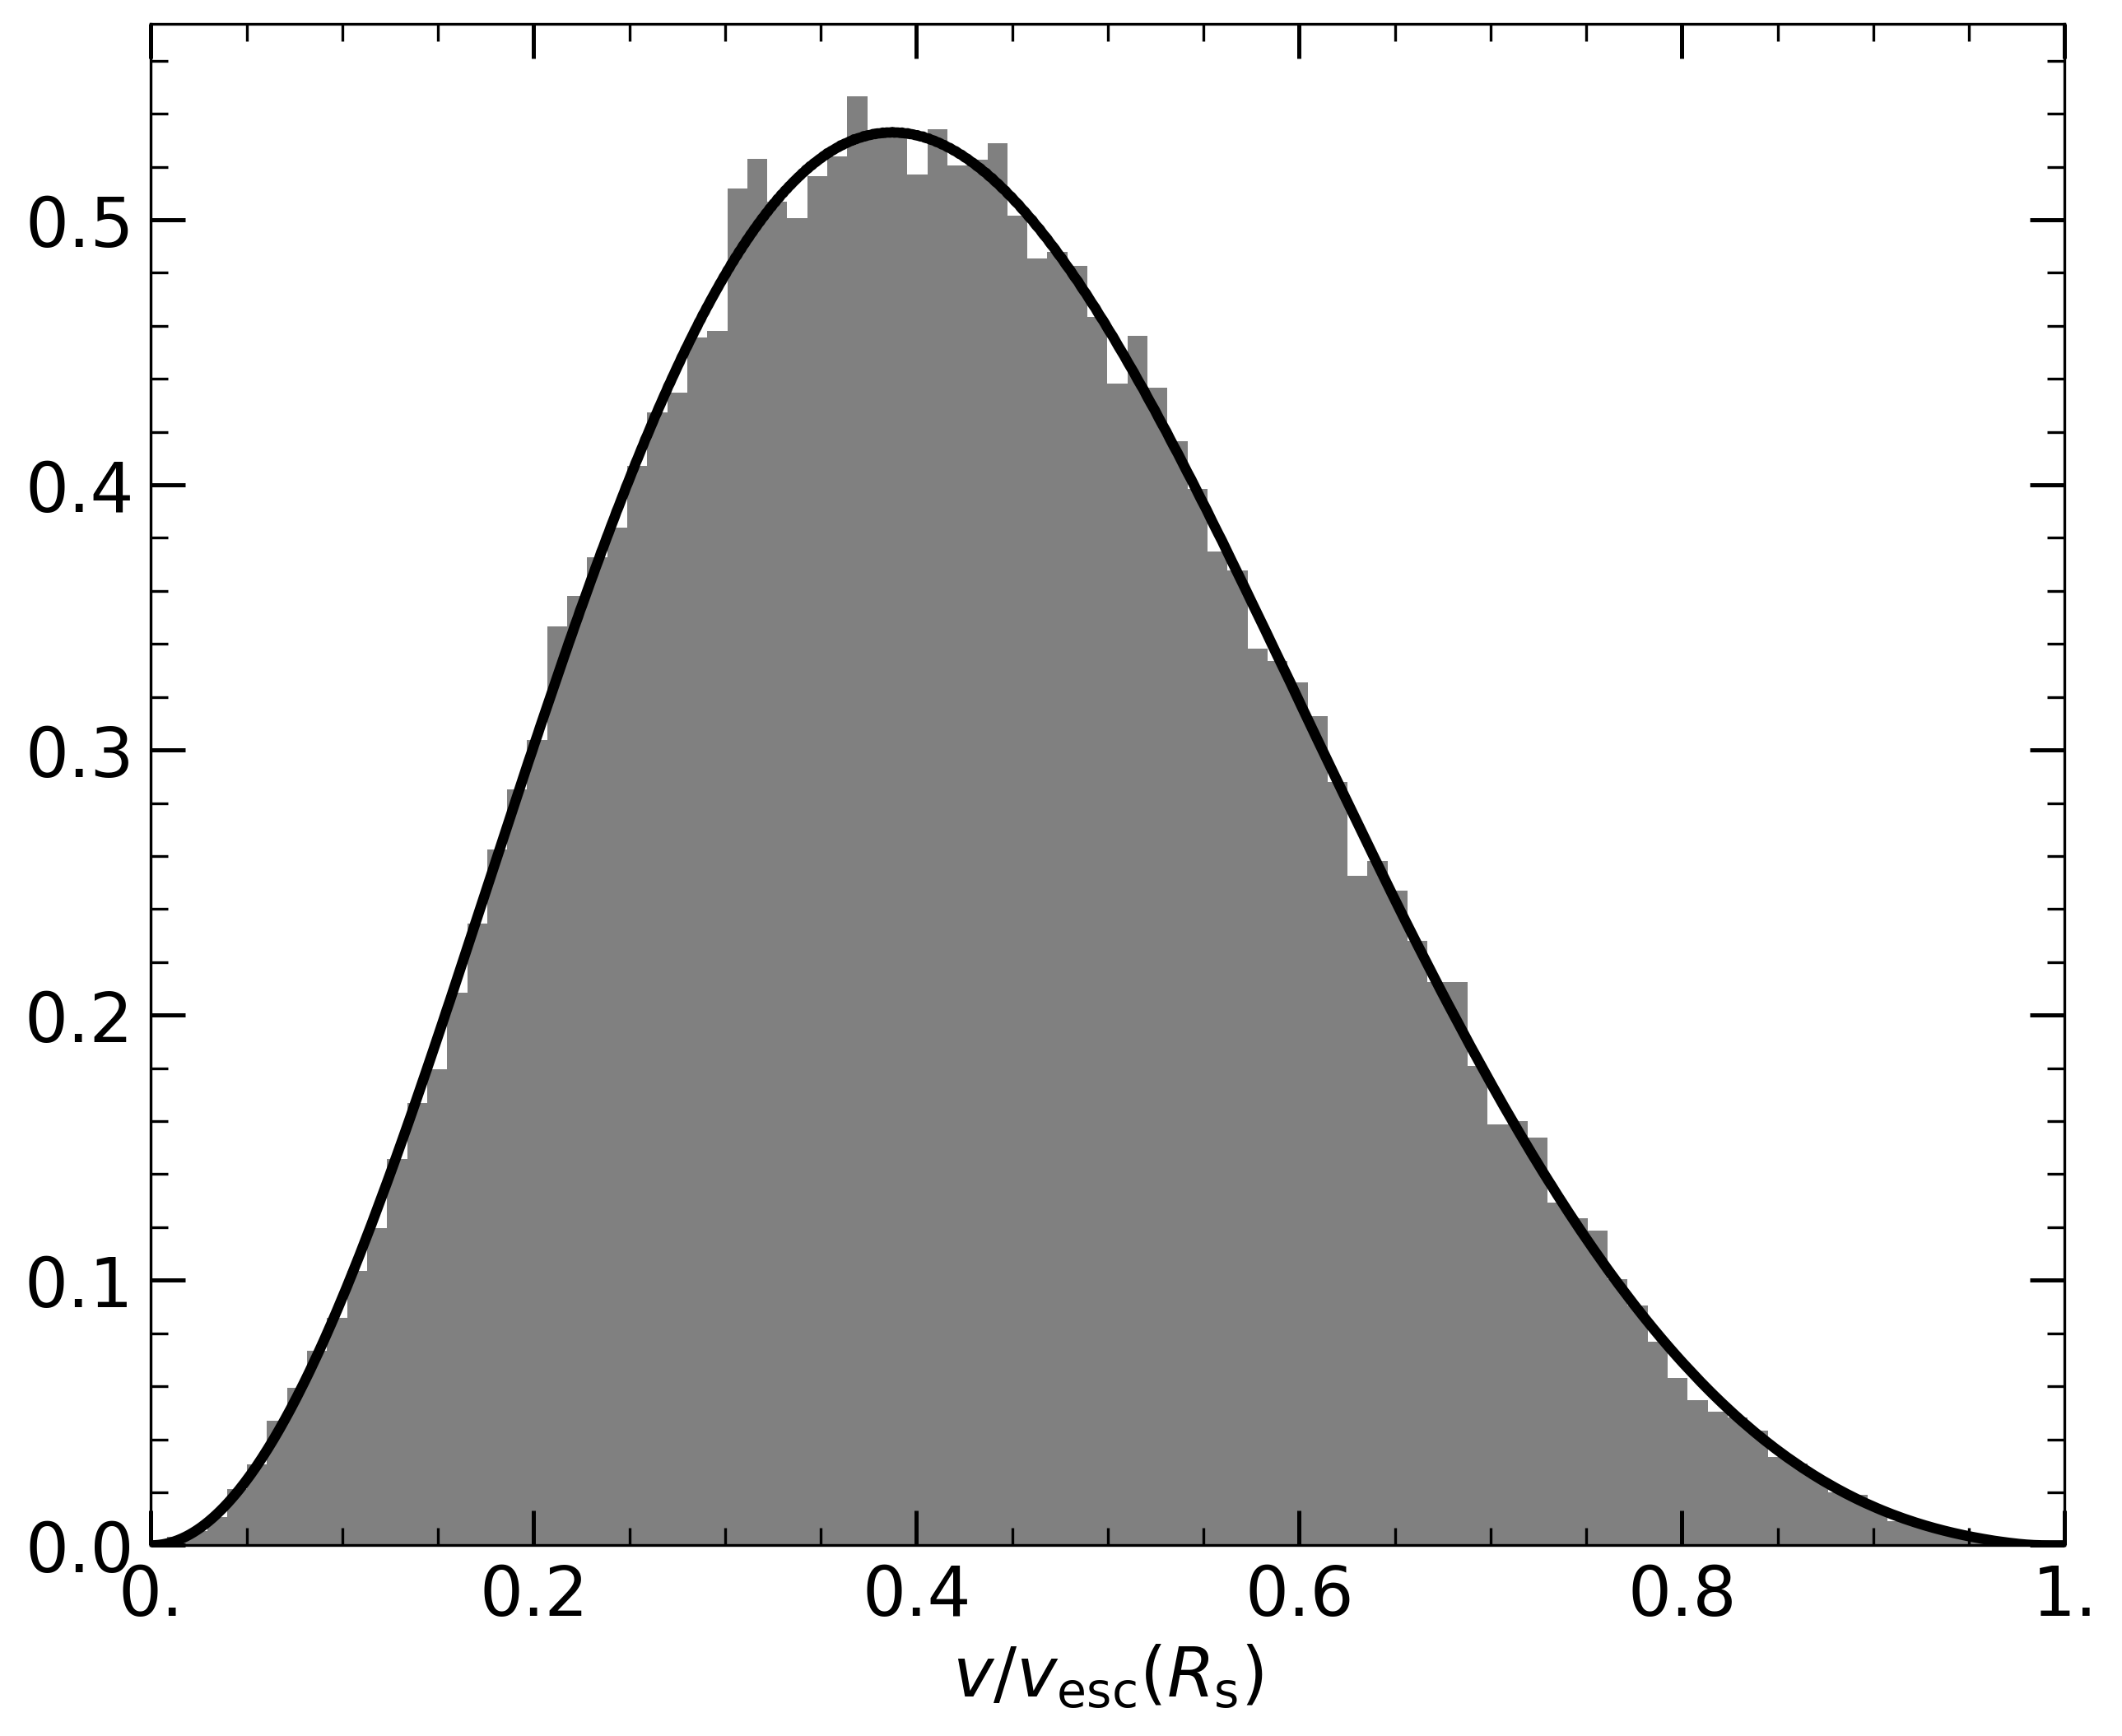
\includegraphics[width=\columnwidth]{images/pdf_v.png}
    \caption{Velocity \acrshort{pdf} at the scale radius \(R_\text{s}\). Same format as in Fig.~\ref{fig:pdf_r}. As noted in Section~\ref{sec:equilibrium_dist}, the velocity \acrshort{pdf} depends on radius. The main effect at increasing radii is a shift of the distribution peak toward lower values, due to the reduced escape velocity, given by \(v_\text{esc}\qty(r) = \sqrt{-2 \phi\qty(r)}\).}
    \label{fig:pdf_v}
\end{figure}

\begin{figure}
    \centering
    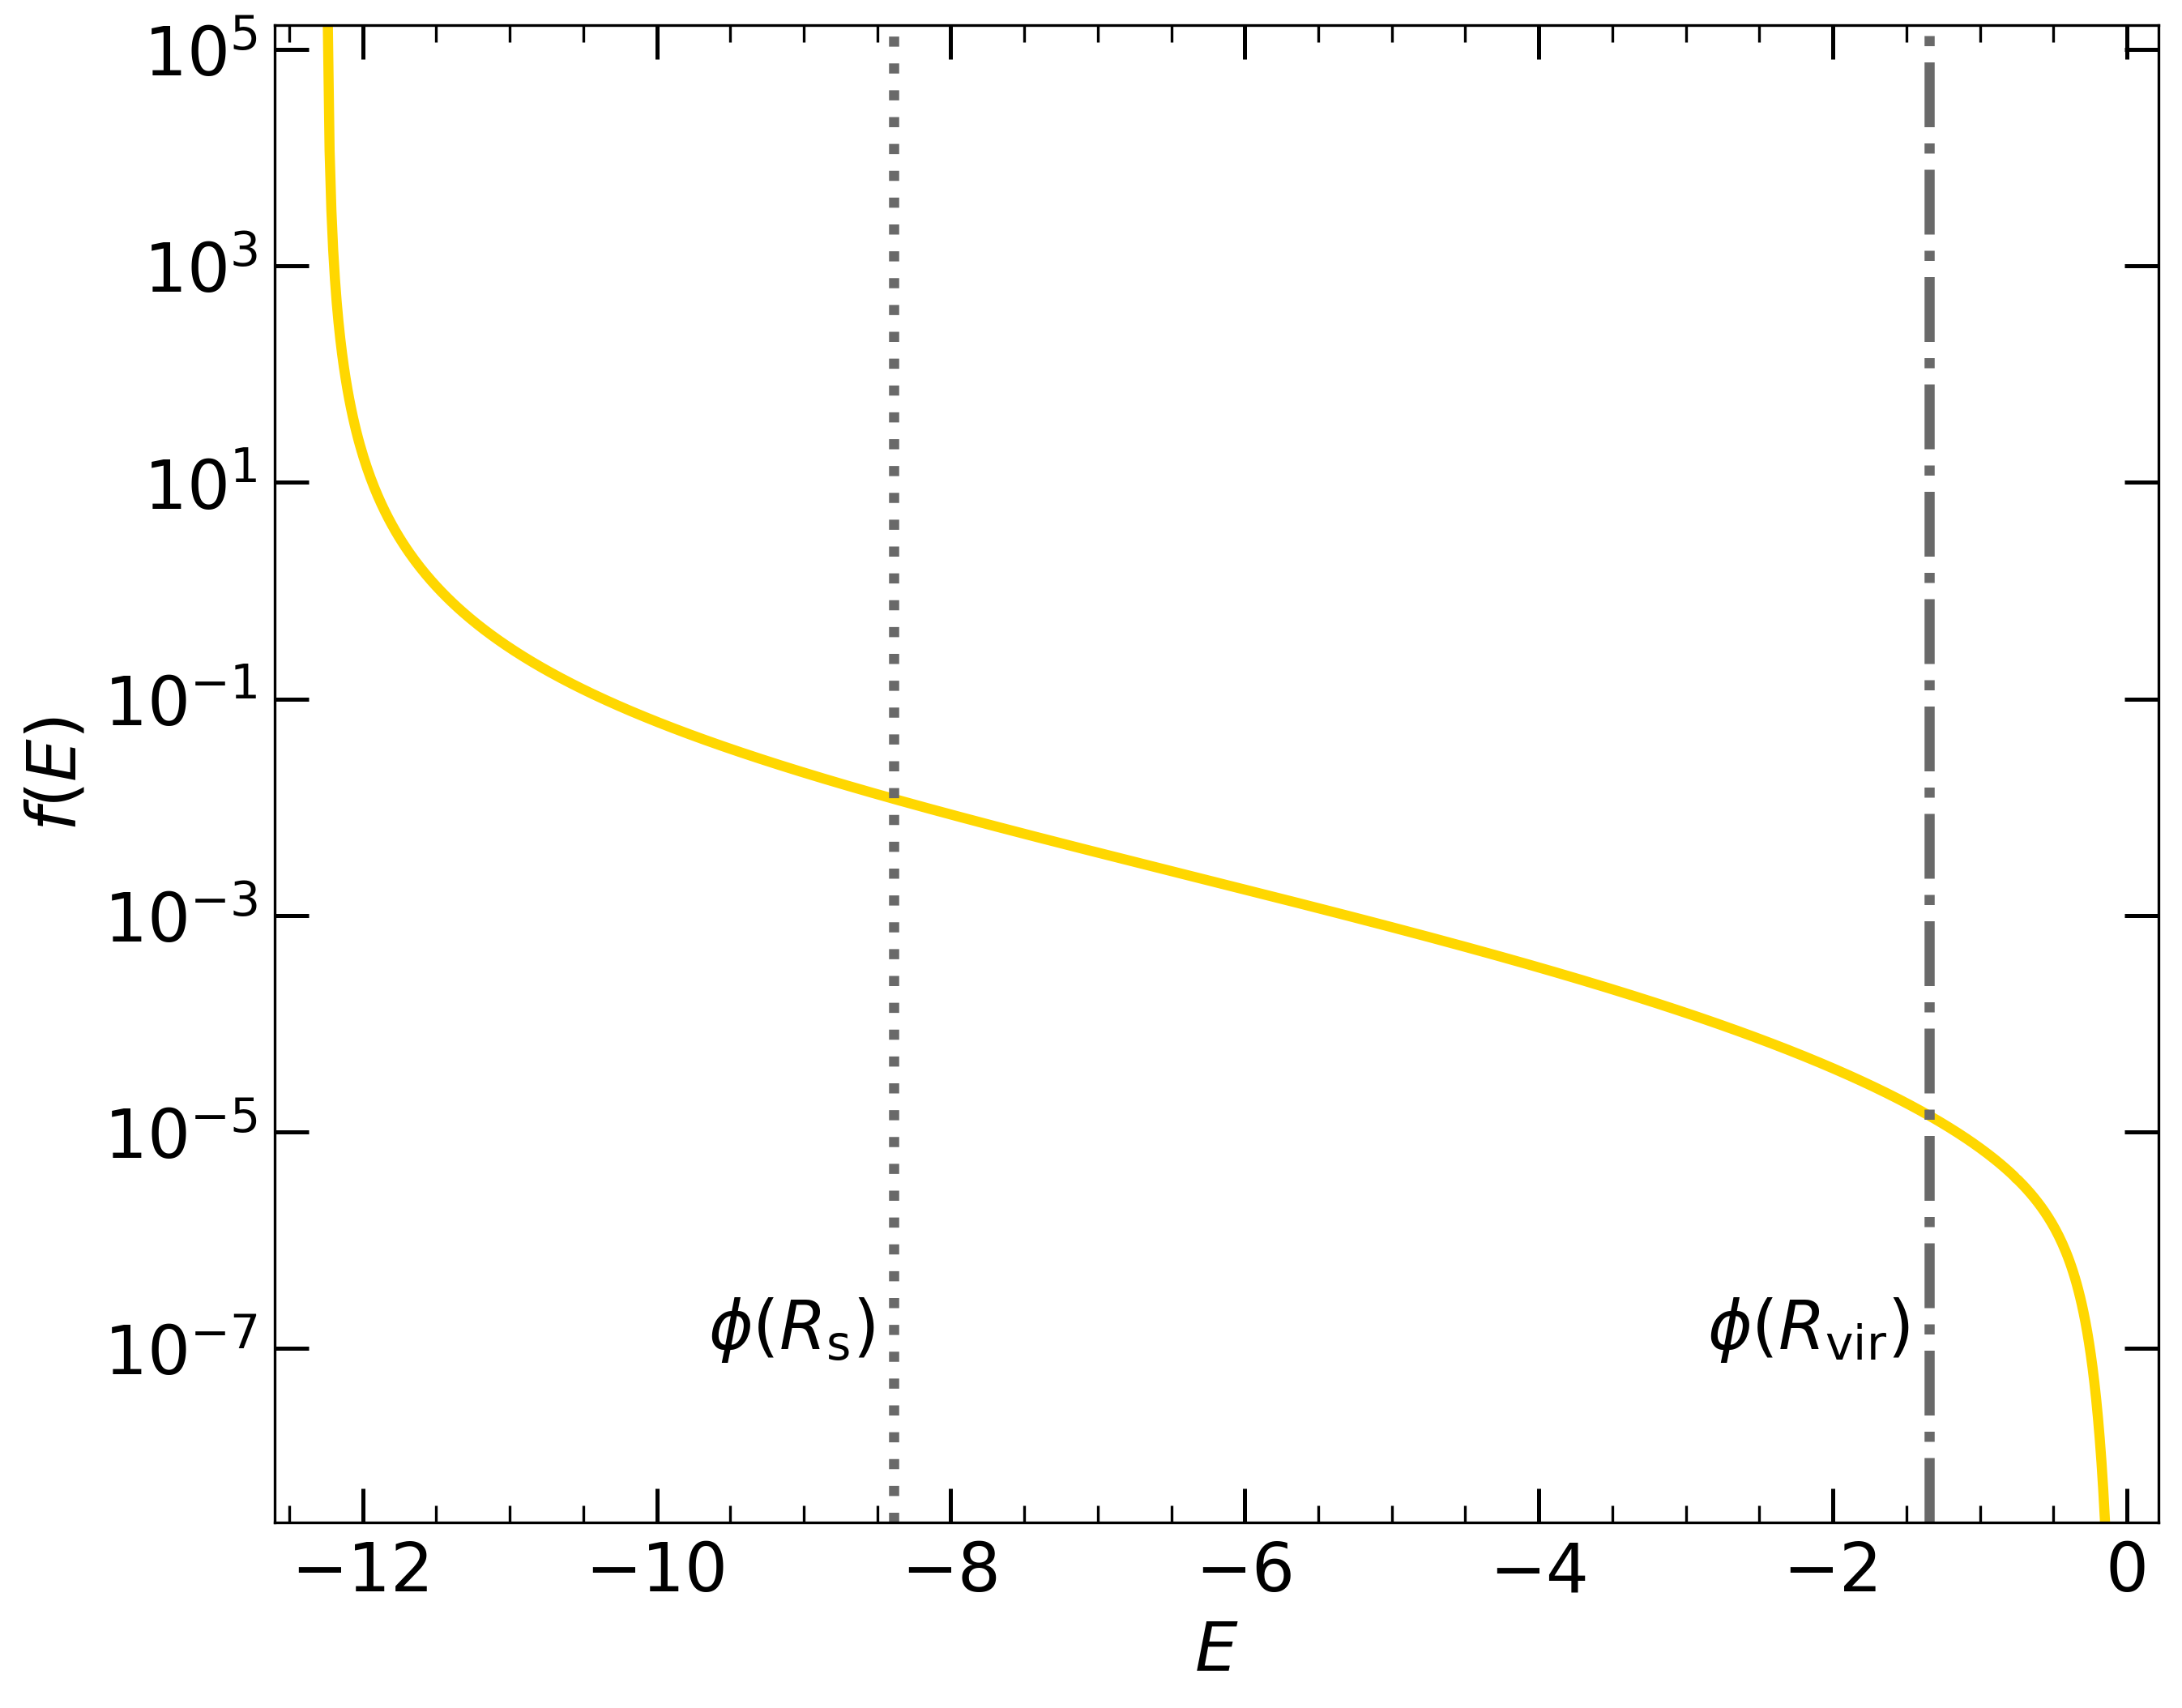
\includegraphics[width=\columnwidth]{images/DF.png}
    \caption{\acrlong{df} computed using Eq.~\ref{eq:edd_inv_r}. The \acrshort{df} is expressed as a function of the total specific energy \(E = v^2/2 + \phi\qty(r)\). The dotted and dashed-dotted vertical lines indicate the potential at the scale radius \(R_\text{s}\) and the virial radius \(R_\text{vir}\), respectively. The energy axis spans the interval \(\qty[\sim \phi\qty(0), \phi\qty(10 R_\text{vir})]\).}
    \label{fig:df}
\end{figure}

\begin{figure}
    \centering
    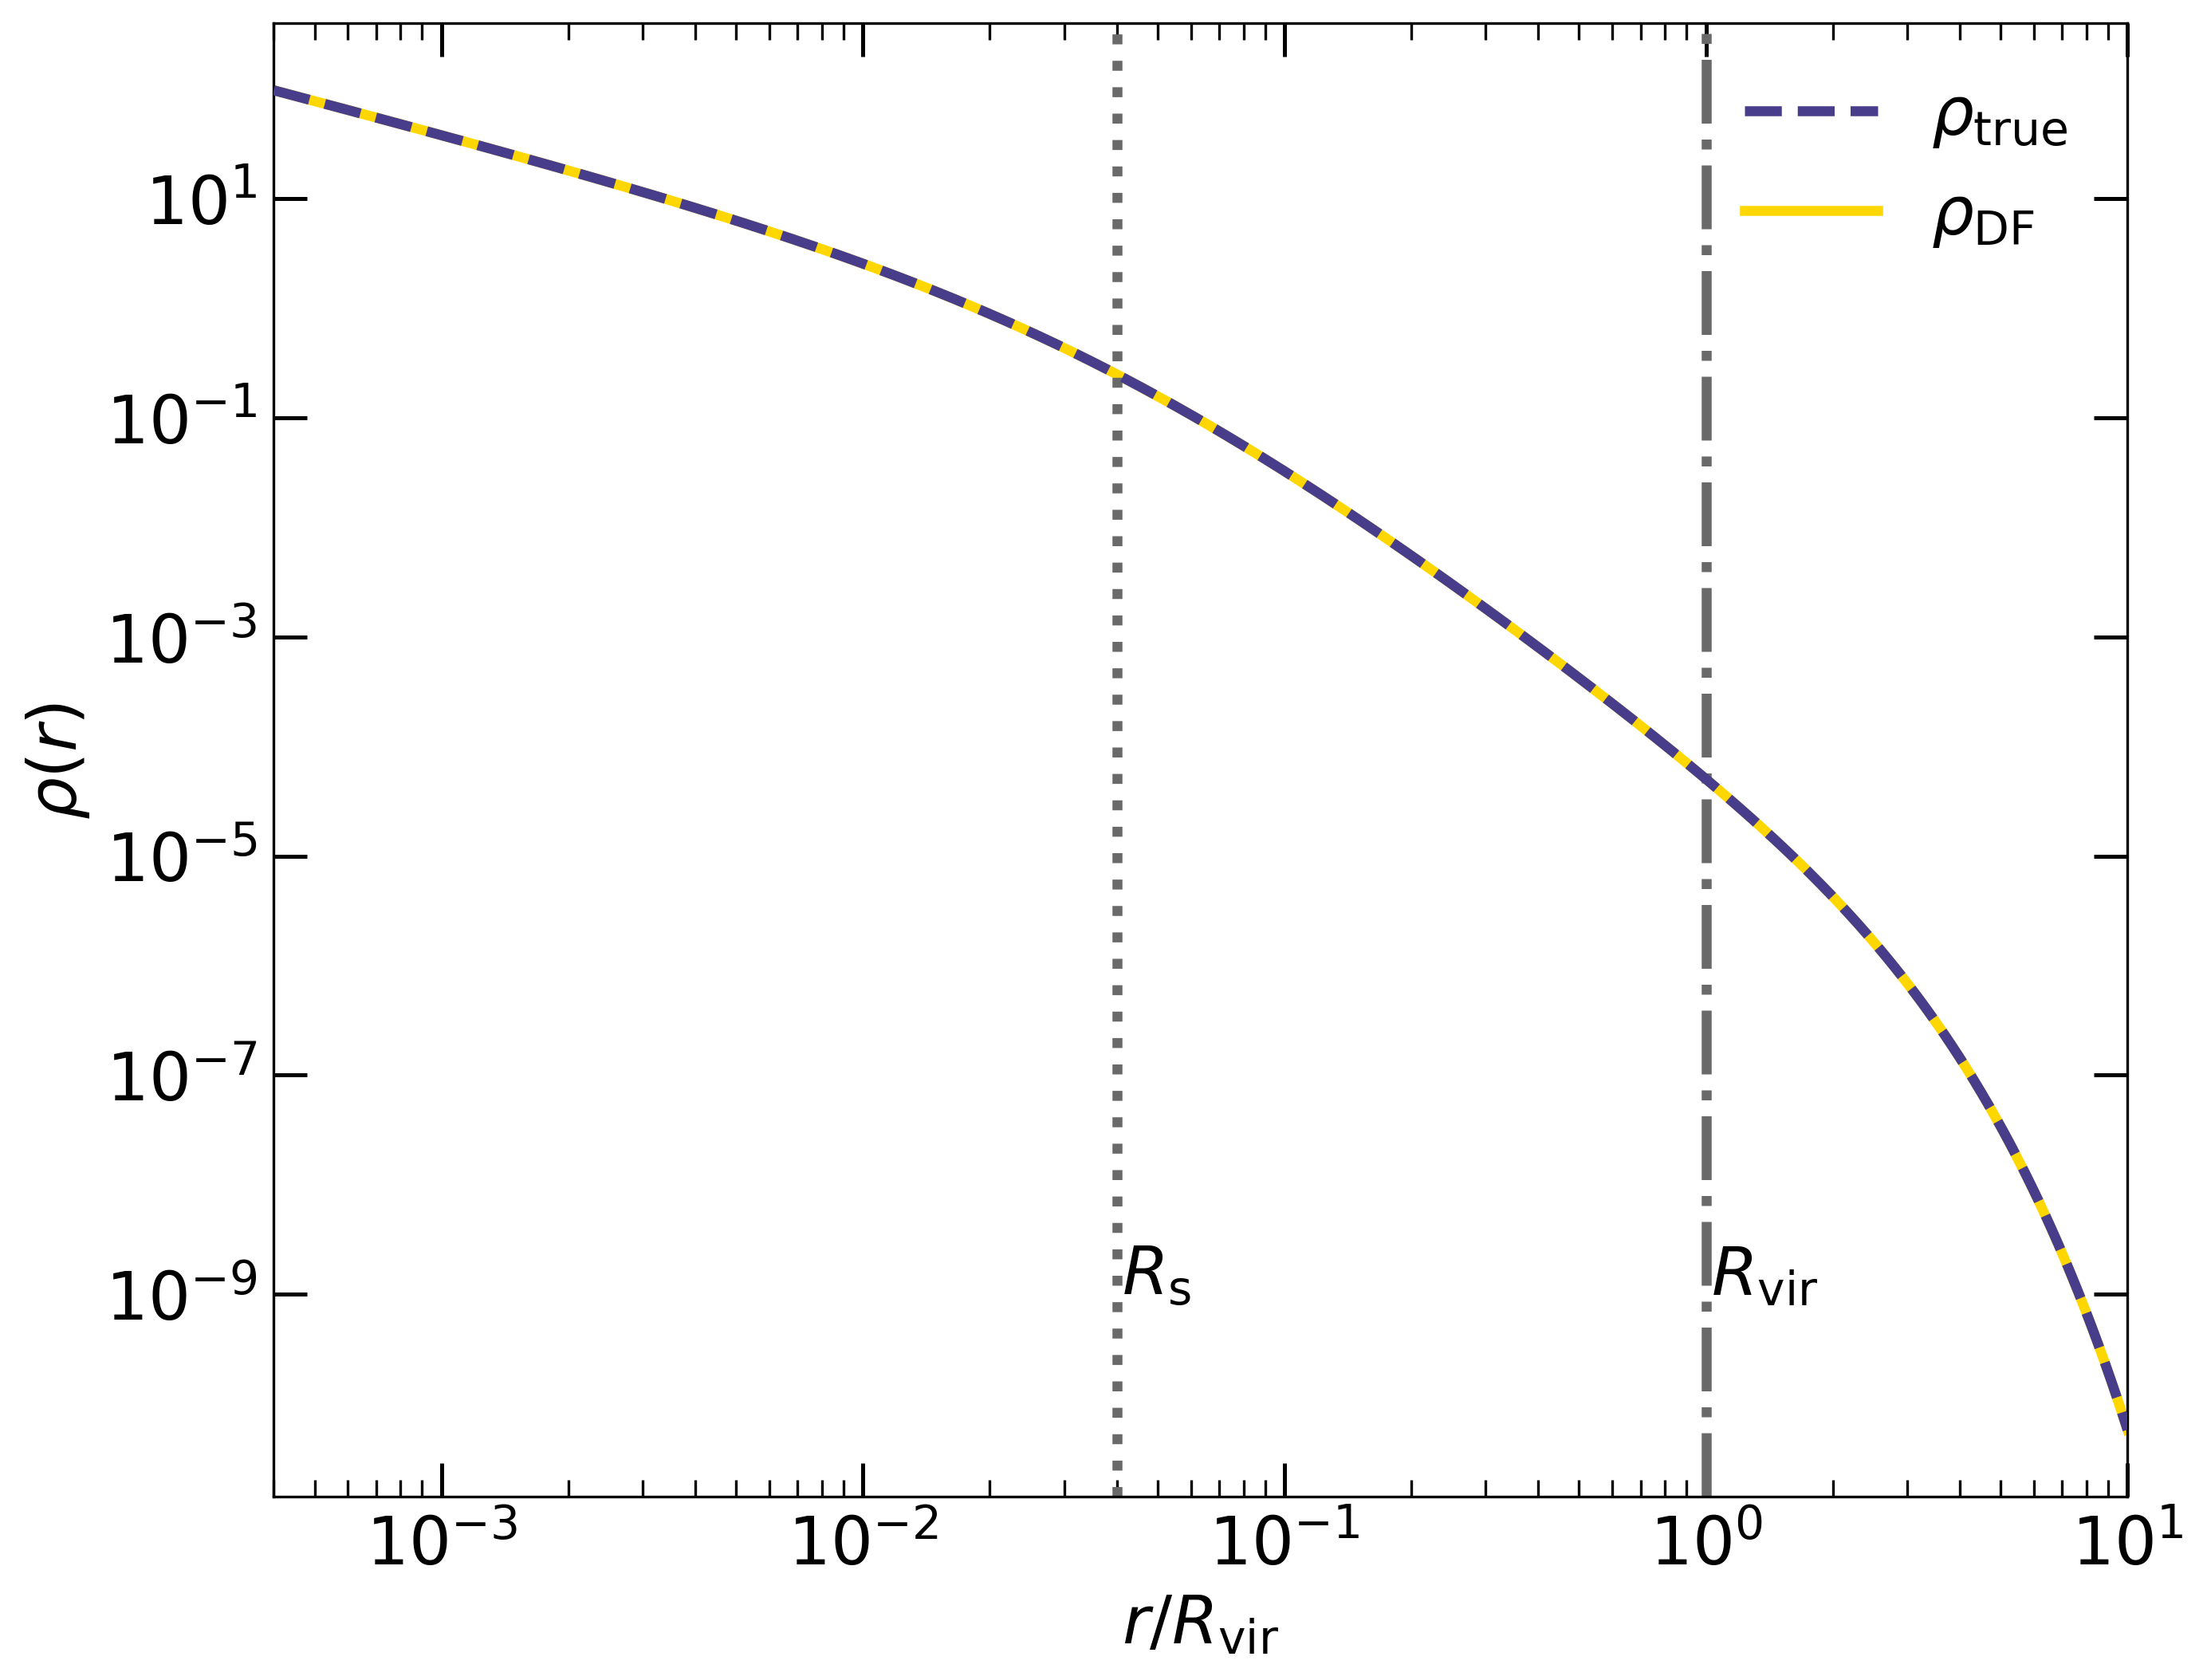
\includegraphics[width=\columnwidth]{images/DF_rho.png}
    \caption{Reconstructed density profile using the fitted \acrshort{krr} \acrshort{df} model. \(\rho_\text{true}\) represents the original density profile (Eq.~\ref{eq:rho}); \(\rho_\text{DF}\) is the density profile reconstructed from the \acrshort{df} via Eq.~\ref{eq:rho_df}.}
    \label{fig:rho_df}
\end{figure}

\subsection{Stability}

The first simulation was designed to test whether the matter distribution obtained from the \acrshort{df} given in Eq.~\ref{eq:edd_inv_r} remains stable over time. To this end, no satellite was added to the distribution, and the stability was assessed by monitoring the Lagrangian radii throughout the simulation. The stopping time was set to \(\sim 10\, t_\text{dyn}\), a value significantly larger than the typical \(t_\text{fric}\) times (Eq.~\ref{eq:t_fric}) used in later simulations involving the perturber.

As shown in Figure~\ref{fig:lag_rad}, the Lagrangian radii remain stable during the simulation, exhibiting only small fluctuations around their mean values. Additionally, the velocity of the center of mass (Figure~\ref{fig:cm_vel}) shows only minor deviations from the initial value, on the order of a few percent. We can therefore conclude that the distribution is stable over the typical timescales considered, and that the numerical accuracy achieved is sufficient for a qualitative analysis of the \acrshort{cdf} and the orbital circularity.

\begin{figure}
    \centering
    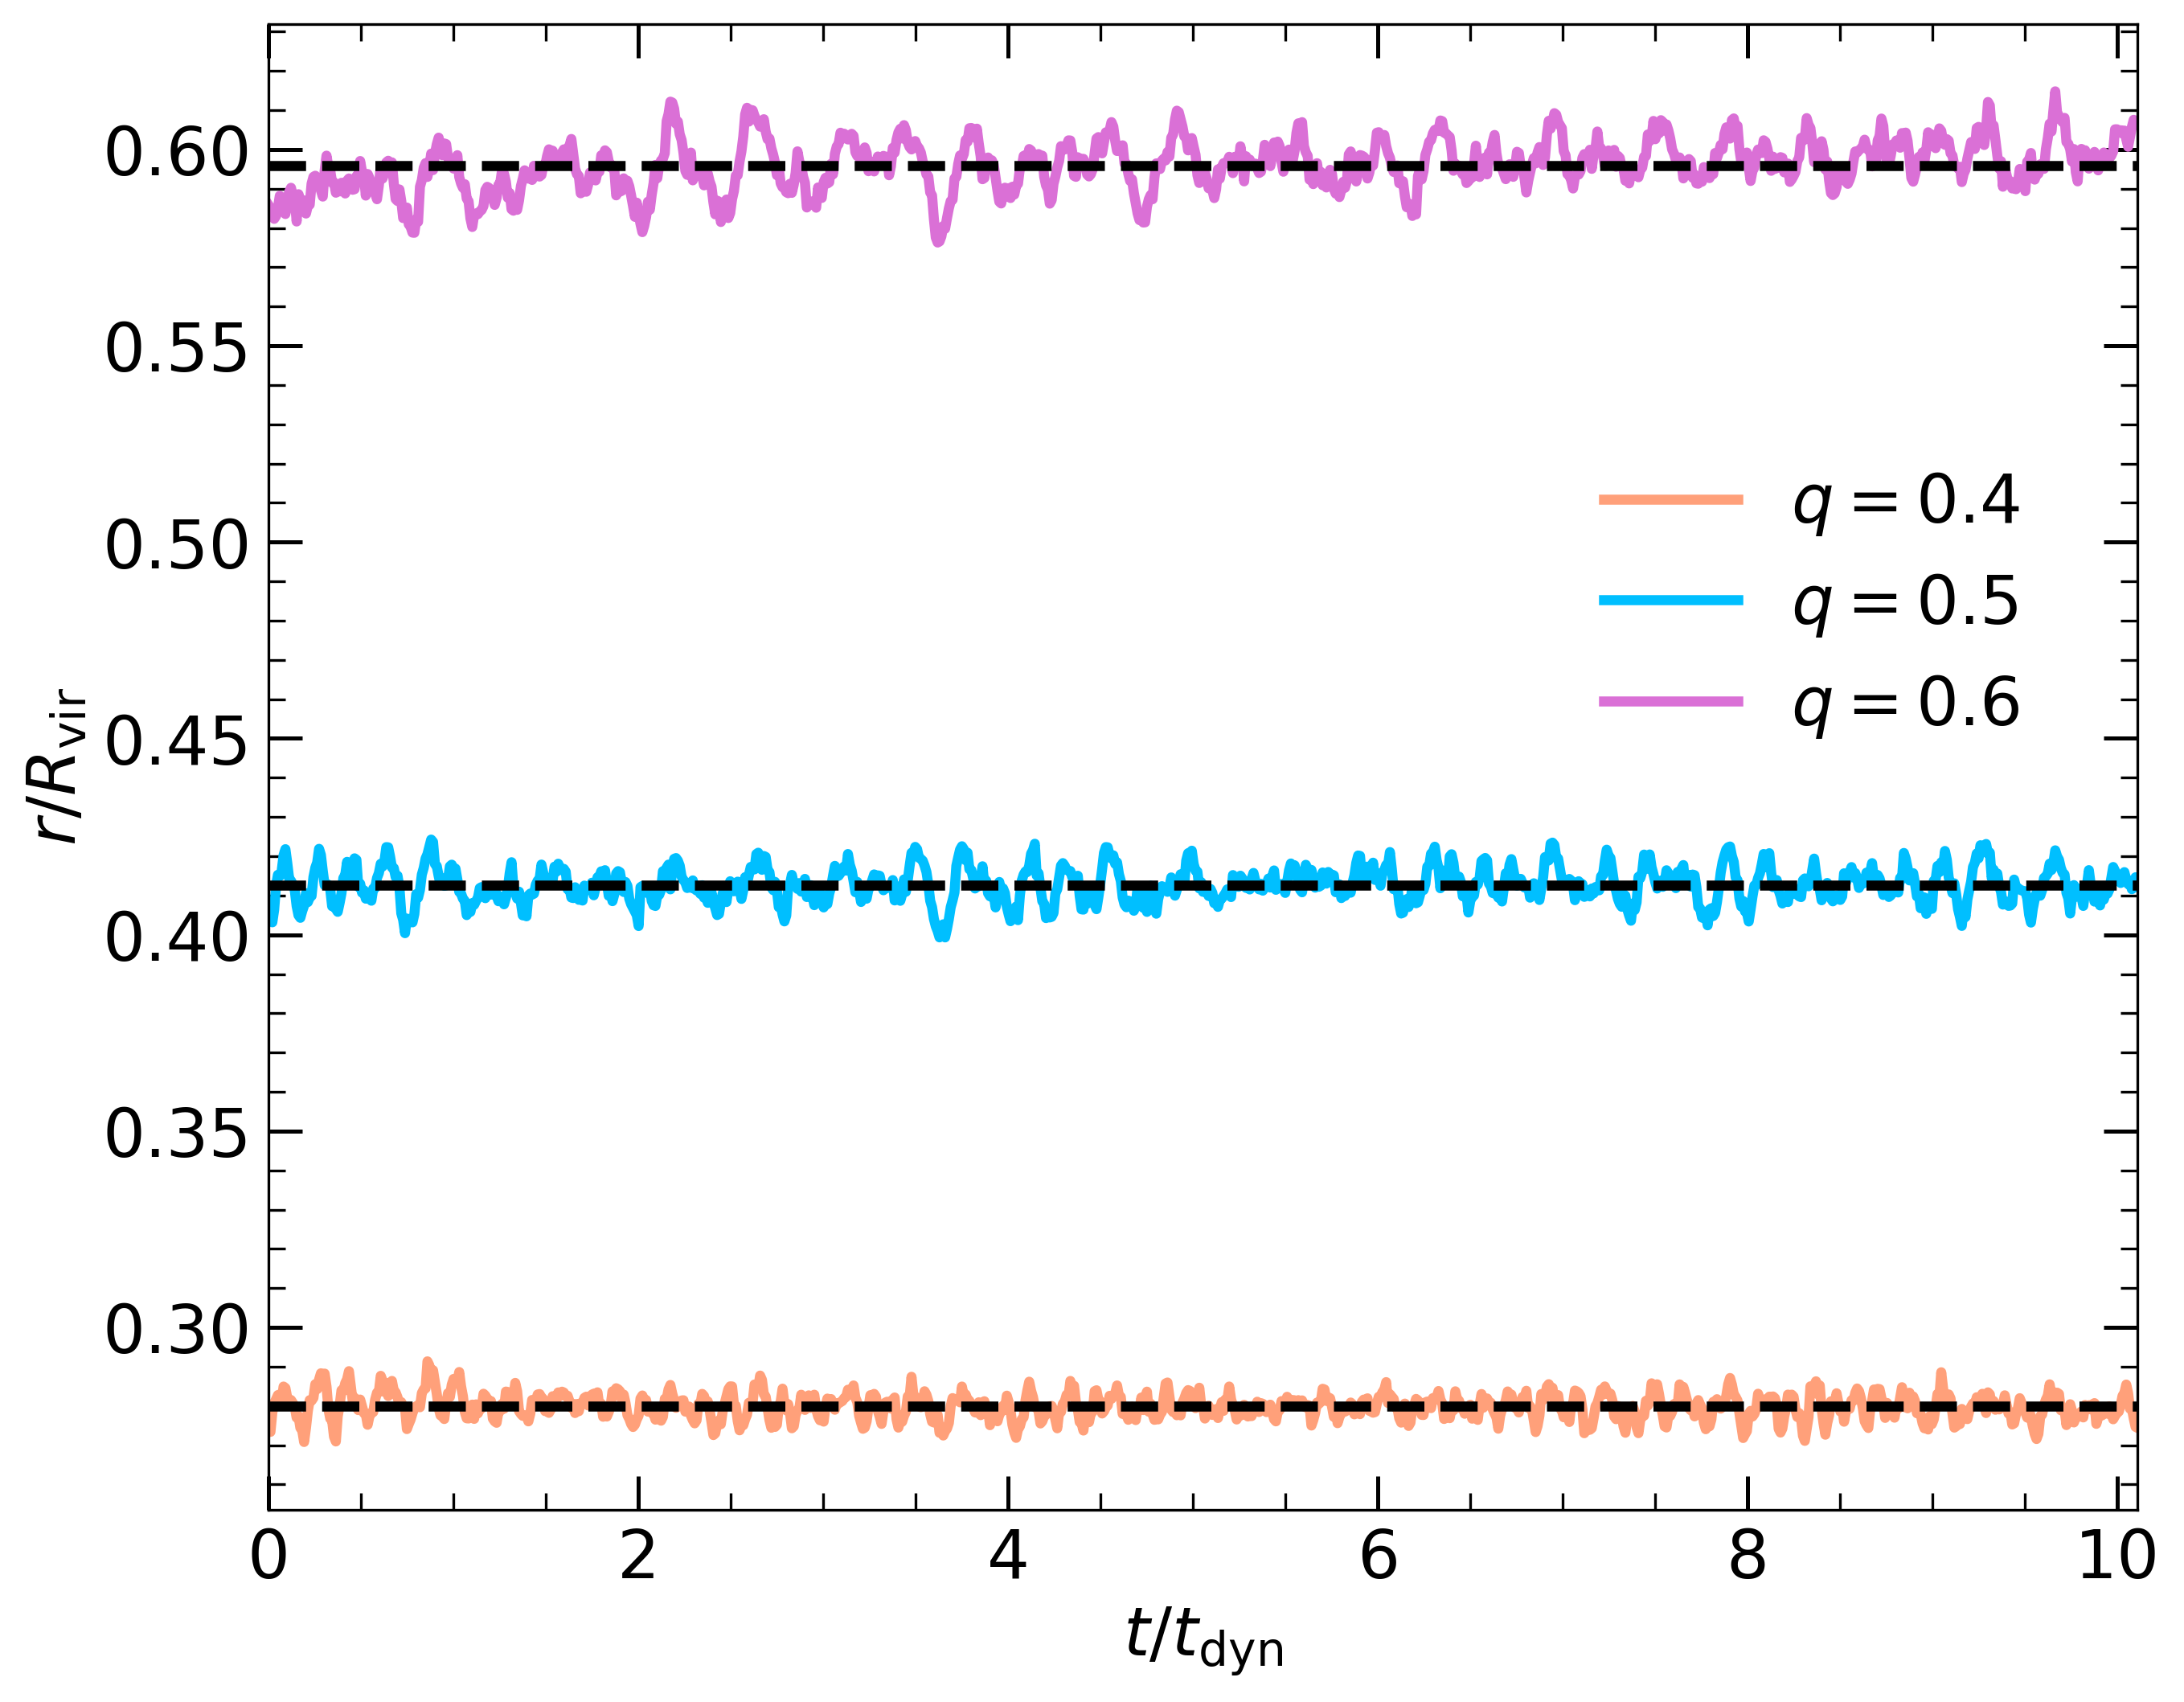
\includegraphics[width=\columnwidth]{images/lag_rad.png}
    \caption{Evolution of the Lagrangian radii. Since the system consists of equal-mass particles, the radii were computed using quantiles (\(q\)) of the distribution of particle distances from the center of mass.}
    \label{fig:lag_rad}
\end{figure}

\begin{figure}
    \centering
    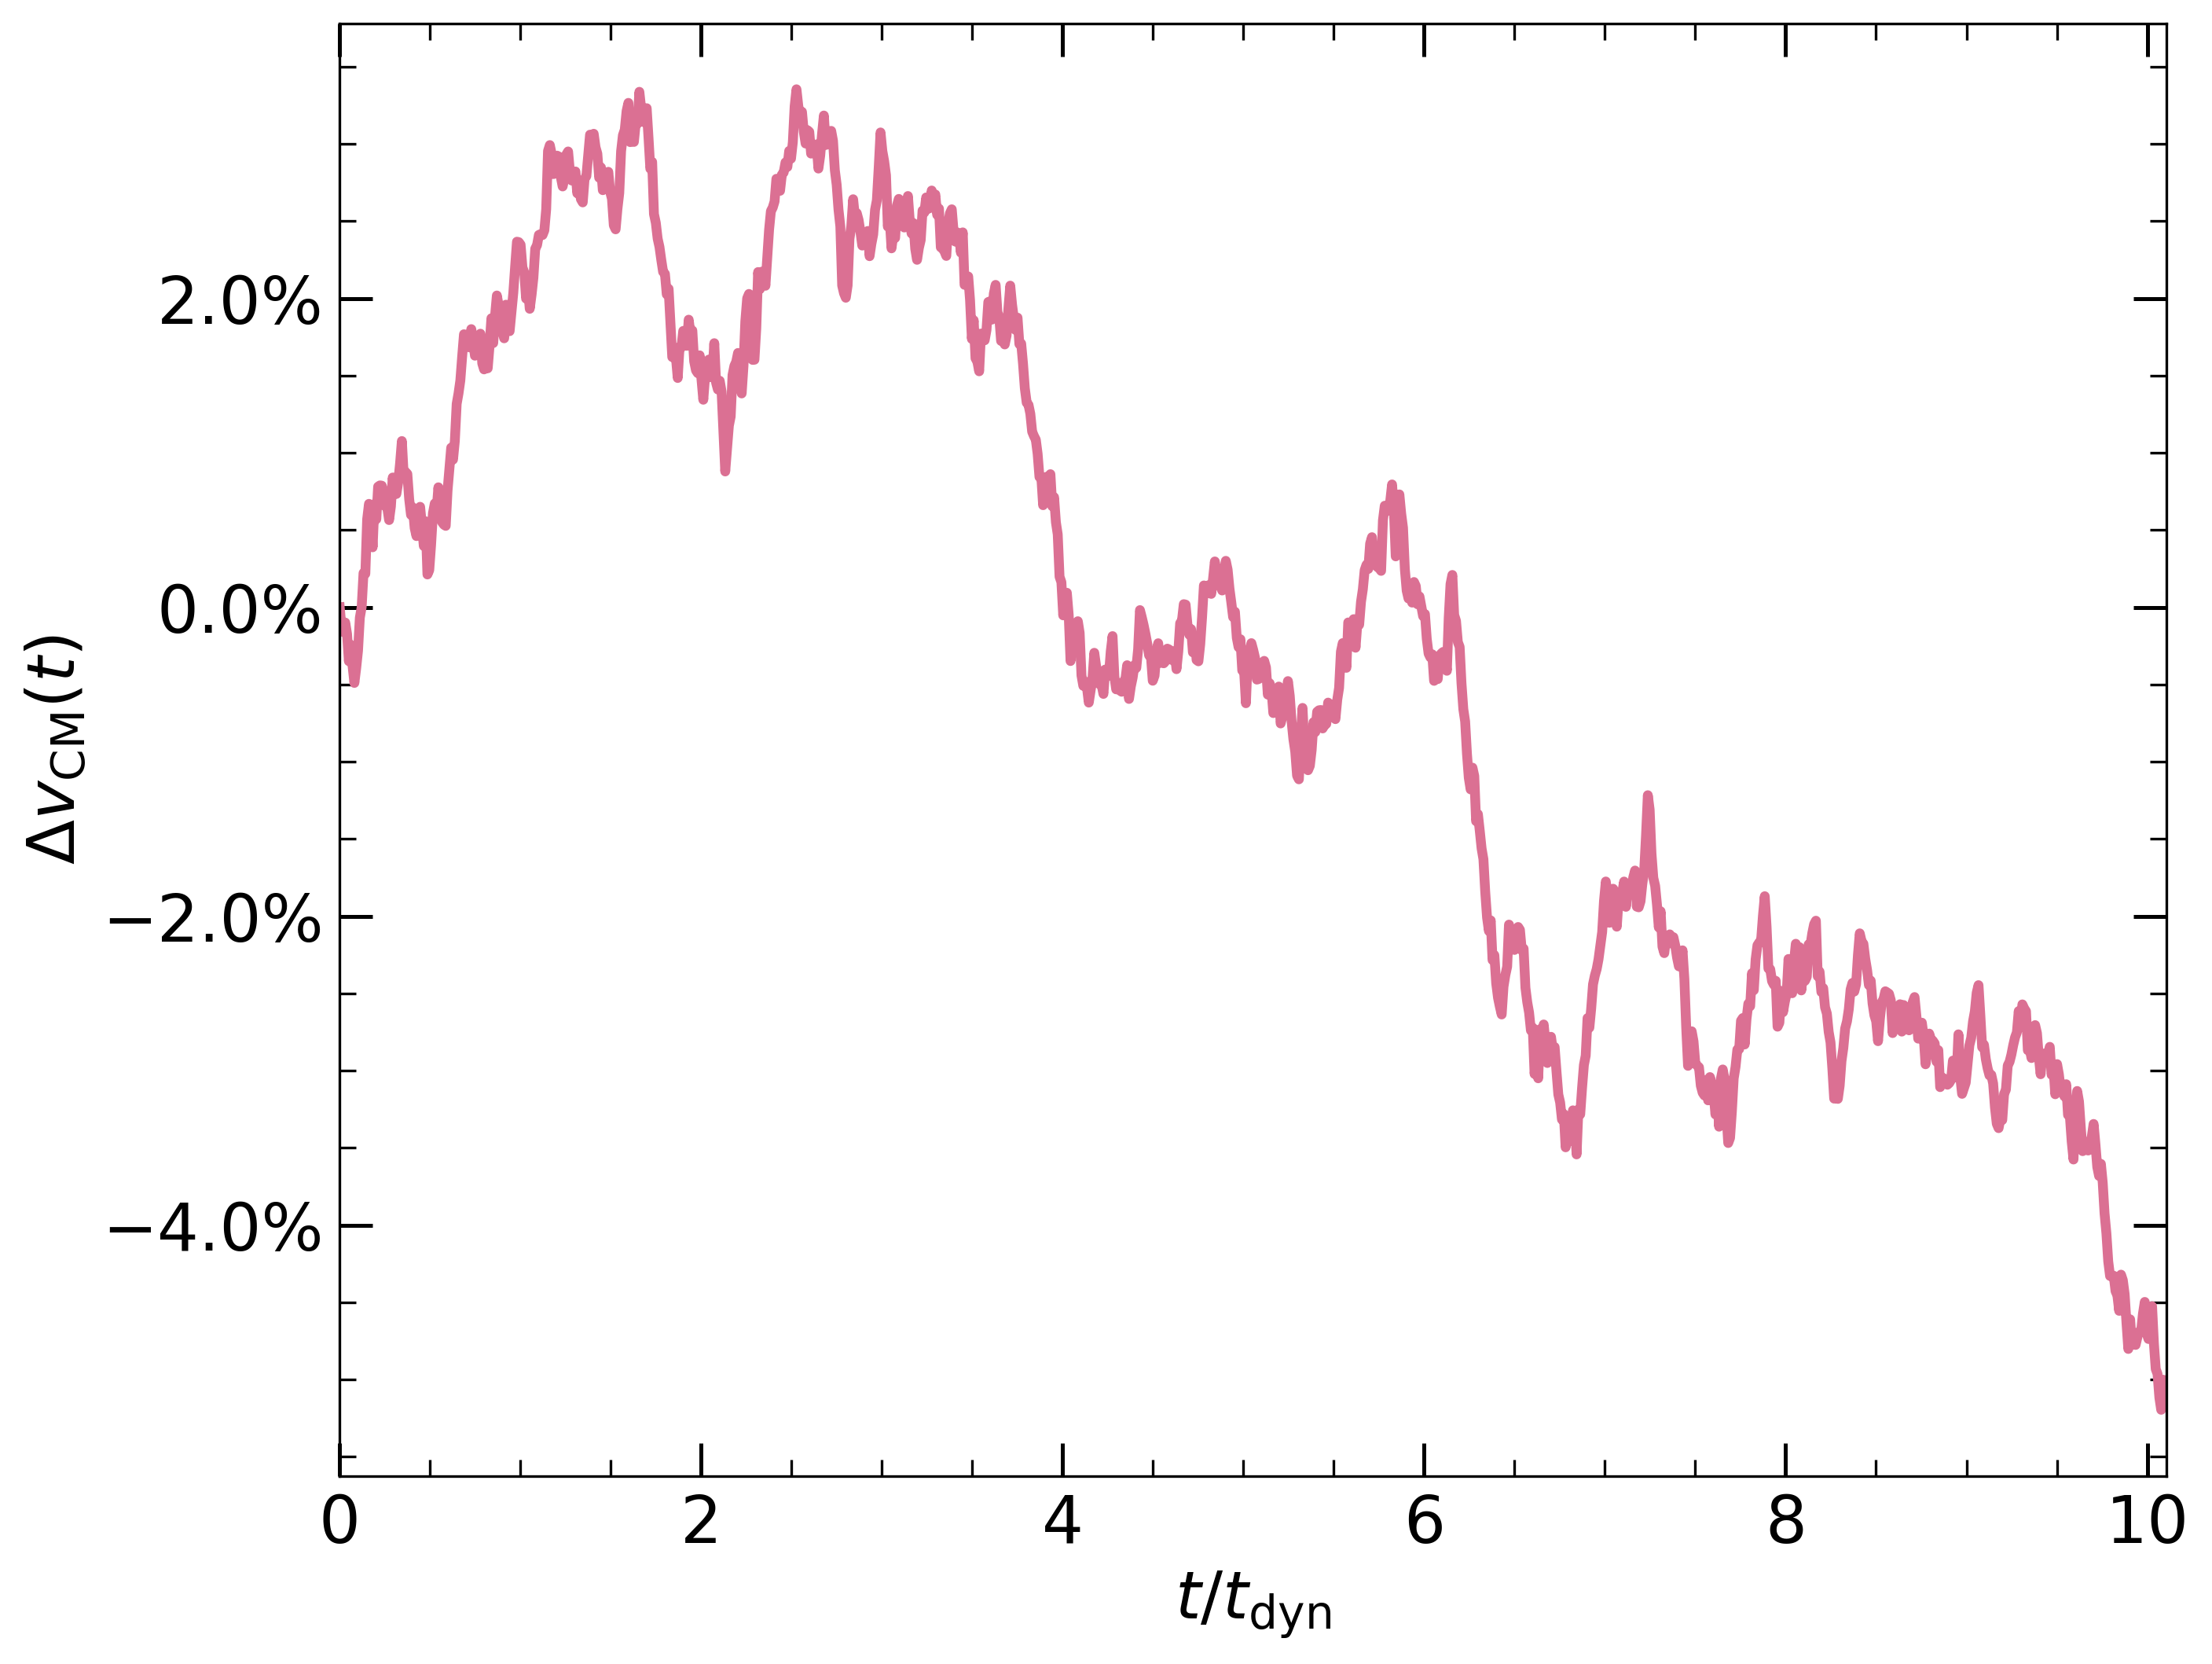
\includegraphics[width=\columnwidth]{images/cm.png}
    \caption{Time evolution of the velocity of the center of mass, expressed as the relative variation from its initial value.}
    \label{fig:cm_vel}
\end{figure}

\subsection{Orbital decay}

We begin by presenting an example of orbital decay for a perturber in the matter distribution. As a reference case, we consider a perturber initialized on a highly eccentric orbit at the virial radius, with mass \(M = M_\text{tot} / 50\) and velocity magnitude equal to the circular velocity at the virial radius. According to Eq.~\ref{eq:t_fric}, the simulation was run for approximately \(3\, t_\text{dyn}\).

Figure~\ref{fig:pert_dist_l} shows the evolution of the perturber’s distance from the center of mass, \(r_p\), and the magnitude of its specific angular momentum, defined as \(\vb{L} = \vb{r}_p \times \vb{v}_p\), where \(\vb{v}_p\) is the perturber's velocity in the center-of-mass reference frame.

\begin{figure}
    \centering
    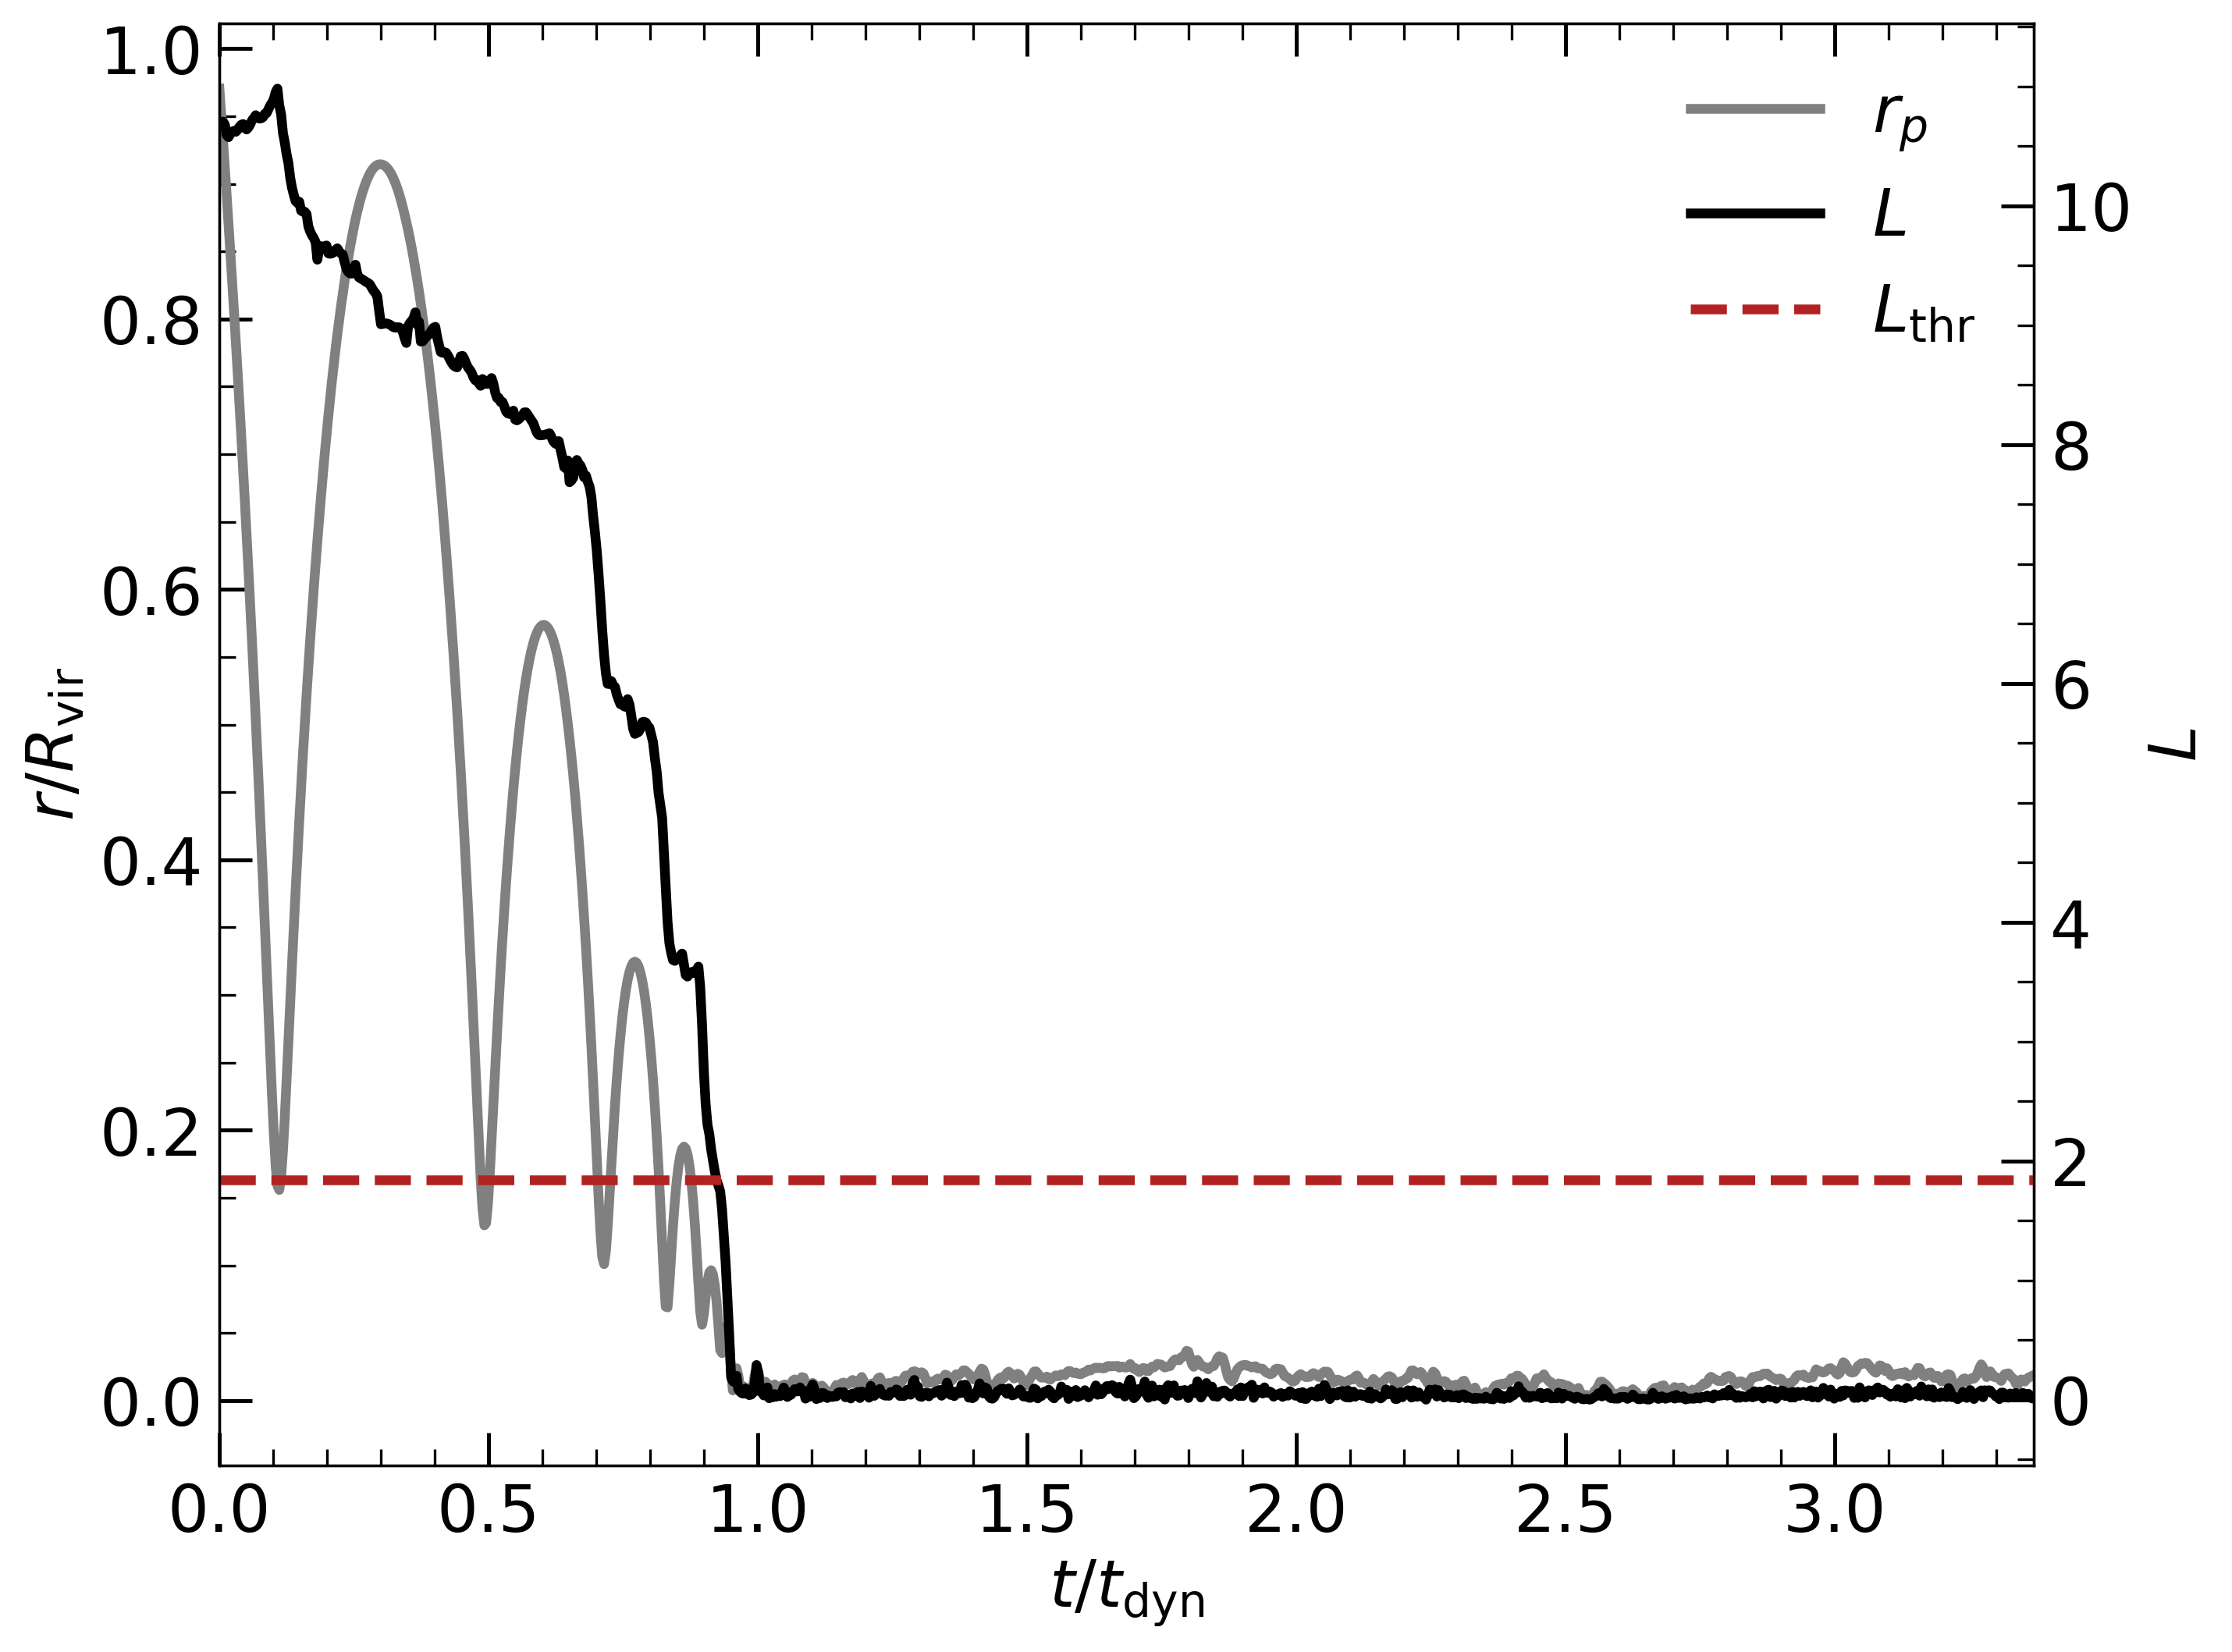
\includegraphics[width=\columnwidth]{images/pert_dist_l.png}
    \caption{Evolution of the distance and specific angular momentum of a \(M_\text{tot} / 50\) perturber relative to the center of mass of the system. \(L_\text{thr}\) is the minimum trusted value for the specific angular momentum, set by the finite resolution of the simulation. It is defined as the specific angular momentum of a circular orbit at the smoothing length radius, multiplied by a constant: \(L_\text{thr} = \zeta \sqrt{\epsilon^3 \phi'(\epsilon)}\), with \(\zeta = 20\) in this case.}
    \label{fig:pert_dist_l}
\end{figure}

The intersection of the black curve with the dashed horizontal line in Figure~\ref{fig:pert_dist_l} defines the time limit considered for the \acrshort{cdf} and circularity analysis. In this example, it corresponds to approximately \(1\, t_\text{dyn}\). Figure~\ref{fig:pert_trajectory} shows the perturber's trajectory projected onto the orbital plane up to this time limit.

\begin{figure}
    \centering
    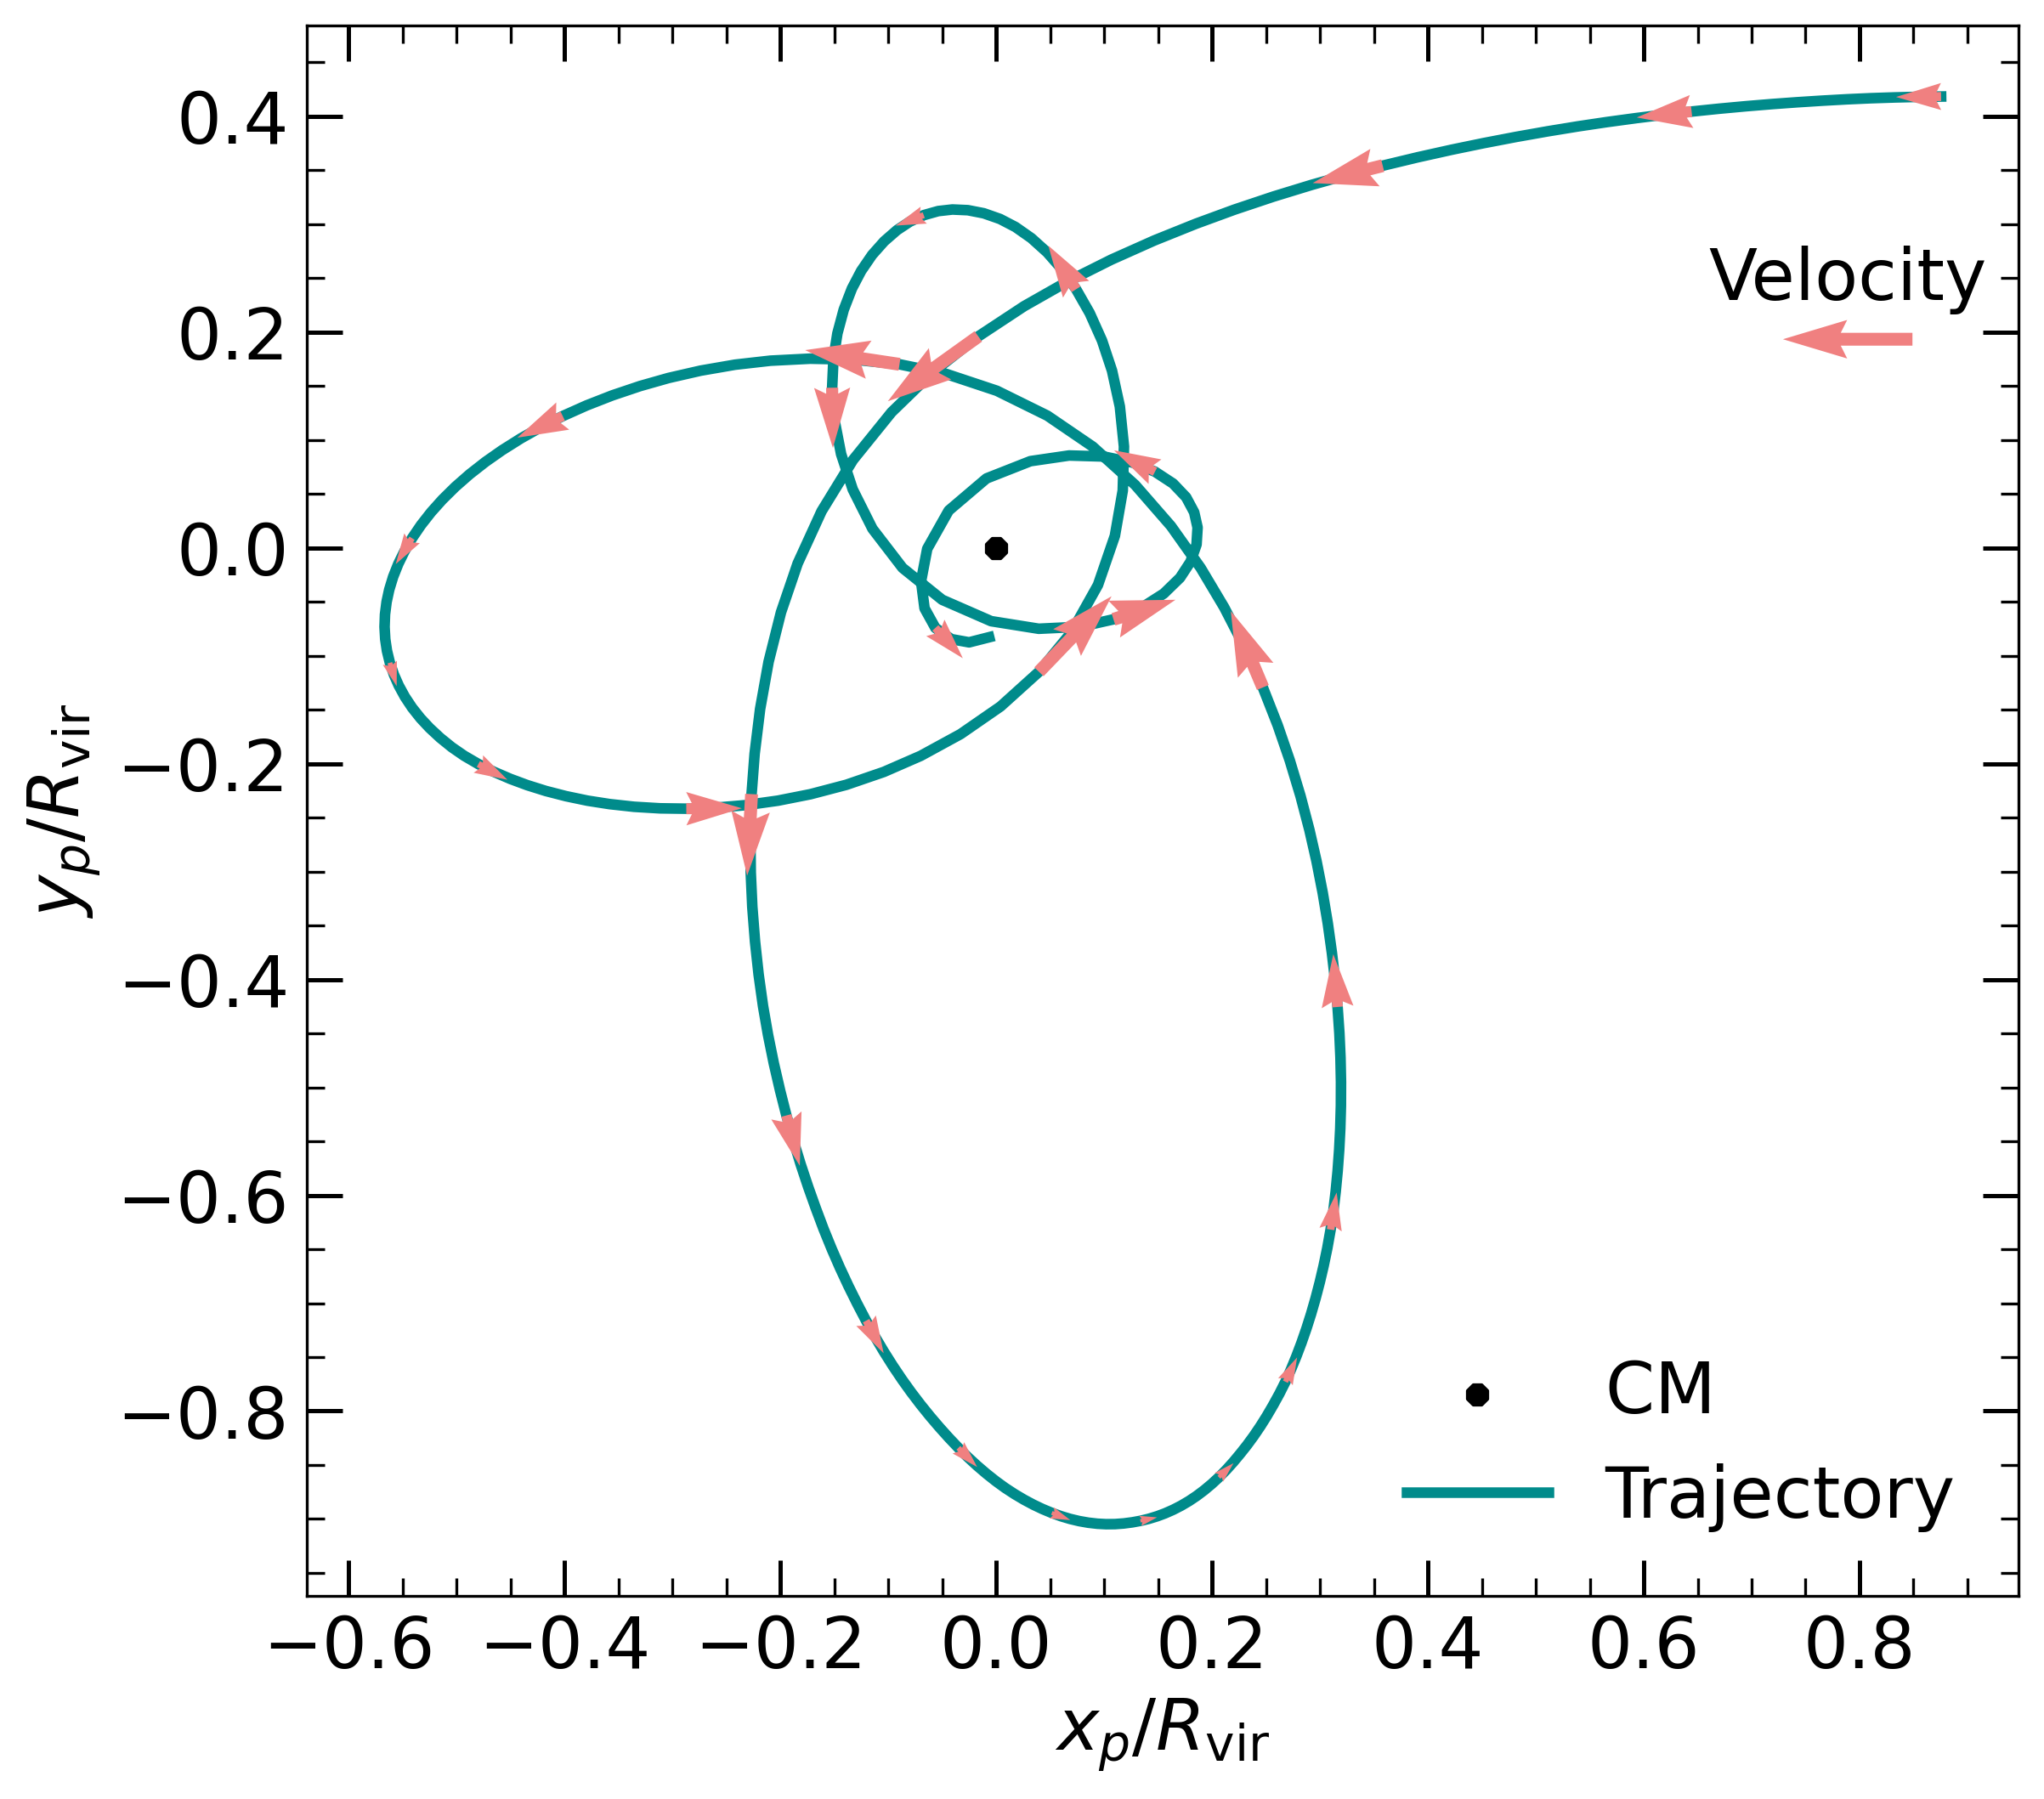
\includegraphics[width=\columnwidth]{images/pert_trajectory.png}
    \caption{Projected trajectory of a \(M_\text{tot} / 50\) perturber in the center-of-mass reference frame. The axes share the same scale. Arrows indicate the perturber’s velocity at various points along the trajectory. The black dot marks the position of the system’s center of mass.}
    \label{fig:pert_trajectory}
\end{figure}

\subsection{\acrlong{cdf}}

To compare the force predicted by the \acrshort{cdf} formula with the actual force experienced by the perturber, we first decompose the instantaneous total acceleration into its components. In a spherically symmetric potential, we can consider two contributions to the total acceleration: one arising from the potential itself—directed toward the center of mass of the distribution—and one due to dissipative forces. Thus, we can write \(\vb{a}_\text{tot} = \vb{a}_r + \vb{a}_\text{diss}\). Knowing the potential and the distance of the perturber from the center of mass, \(r_p\), we have:
\[
\vb{a}_r = -\grad{\phi(r_p)} = -\phi'(r_p) \vu{r}_p,
\]
and therefore, at each simulation snapshot, the dissipative component of the acceleration is given by:
\begin{equation}
    \vb{a}_\text{diss} = \vb{a}_\text{tot} + \phi'(r_p) \vu{r}_p.
    \label{eq:a_diss}
\end{equation}

While the \acrshort{cdf} force is always directed opposite to the motion of the perturber, the actual dissipative force computed via Eq.~\ref{eq:a_diss} has a direction determined by the local dynamics of the system and may thus display more complex behavior. Figure~\ref{fig:pert_snap_forces} shows a snapshot of the perturber’s orbit, along with the components of the acceleration derived from Eq.~\ref{eq:a_diss}.

\begin{figure}
    \centering
    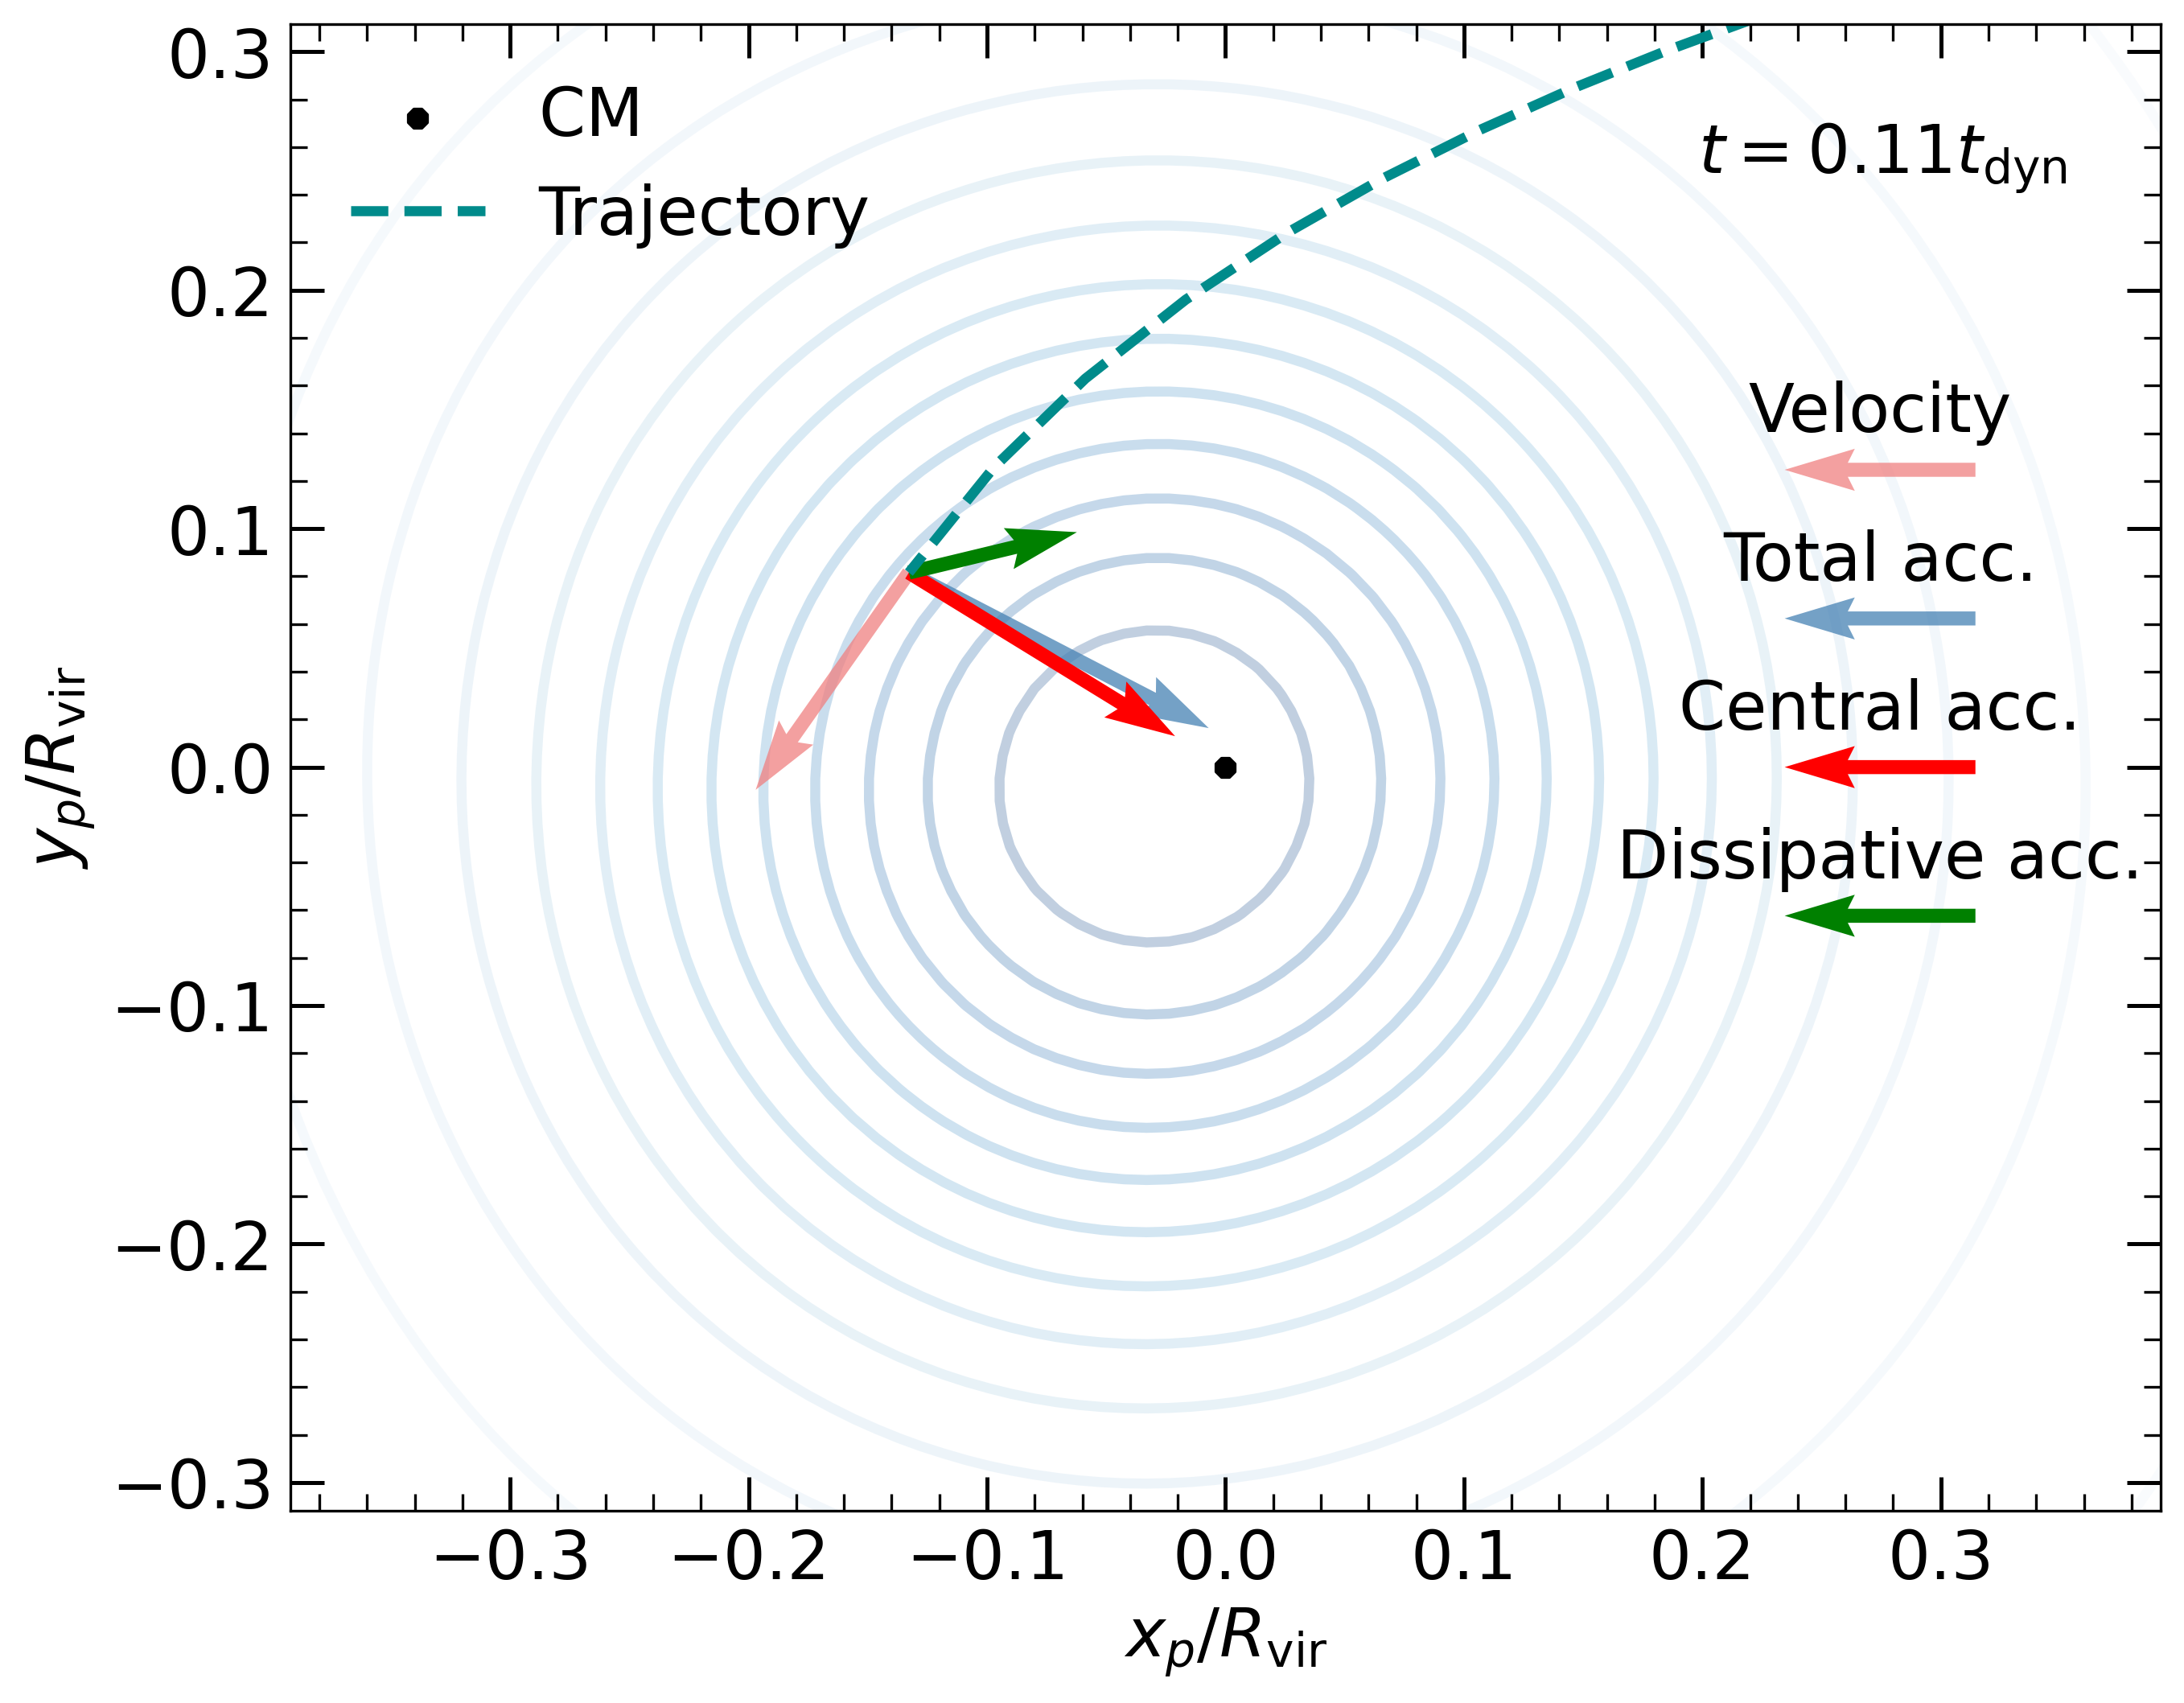
\includegraphics[width=\columnwidth]{images/pert_snapshot_forces.png}
    \caption{Snapshot of the first pericenter passage of a \(M_\text{tot} / 50\) perturber in the center-of-mass reference frame. The axes share the same scale, but arrow lengths have been rescaled non-uniformly for visualization purposes. Contour levels represent the projected density on the orbital plane.}
    \label{fig:pert_snap_forces}
\end{figure}

Nonetheless, we can compare the magnitudes of \(\vb{a}_\text{diss}\) and the \acrshort{cdf}, as shown in Figure~\ref{fig:pert_acc_cdf}.

\begin{figure}
    \centering
    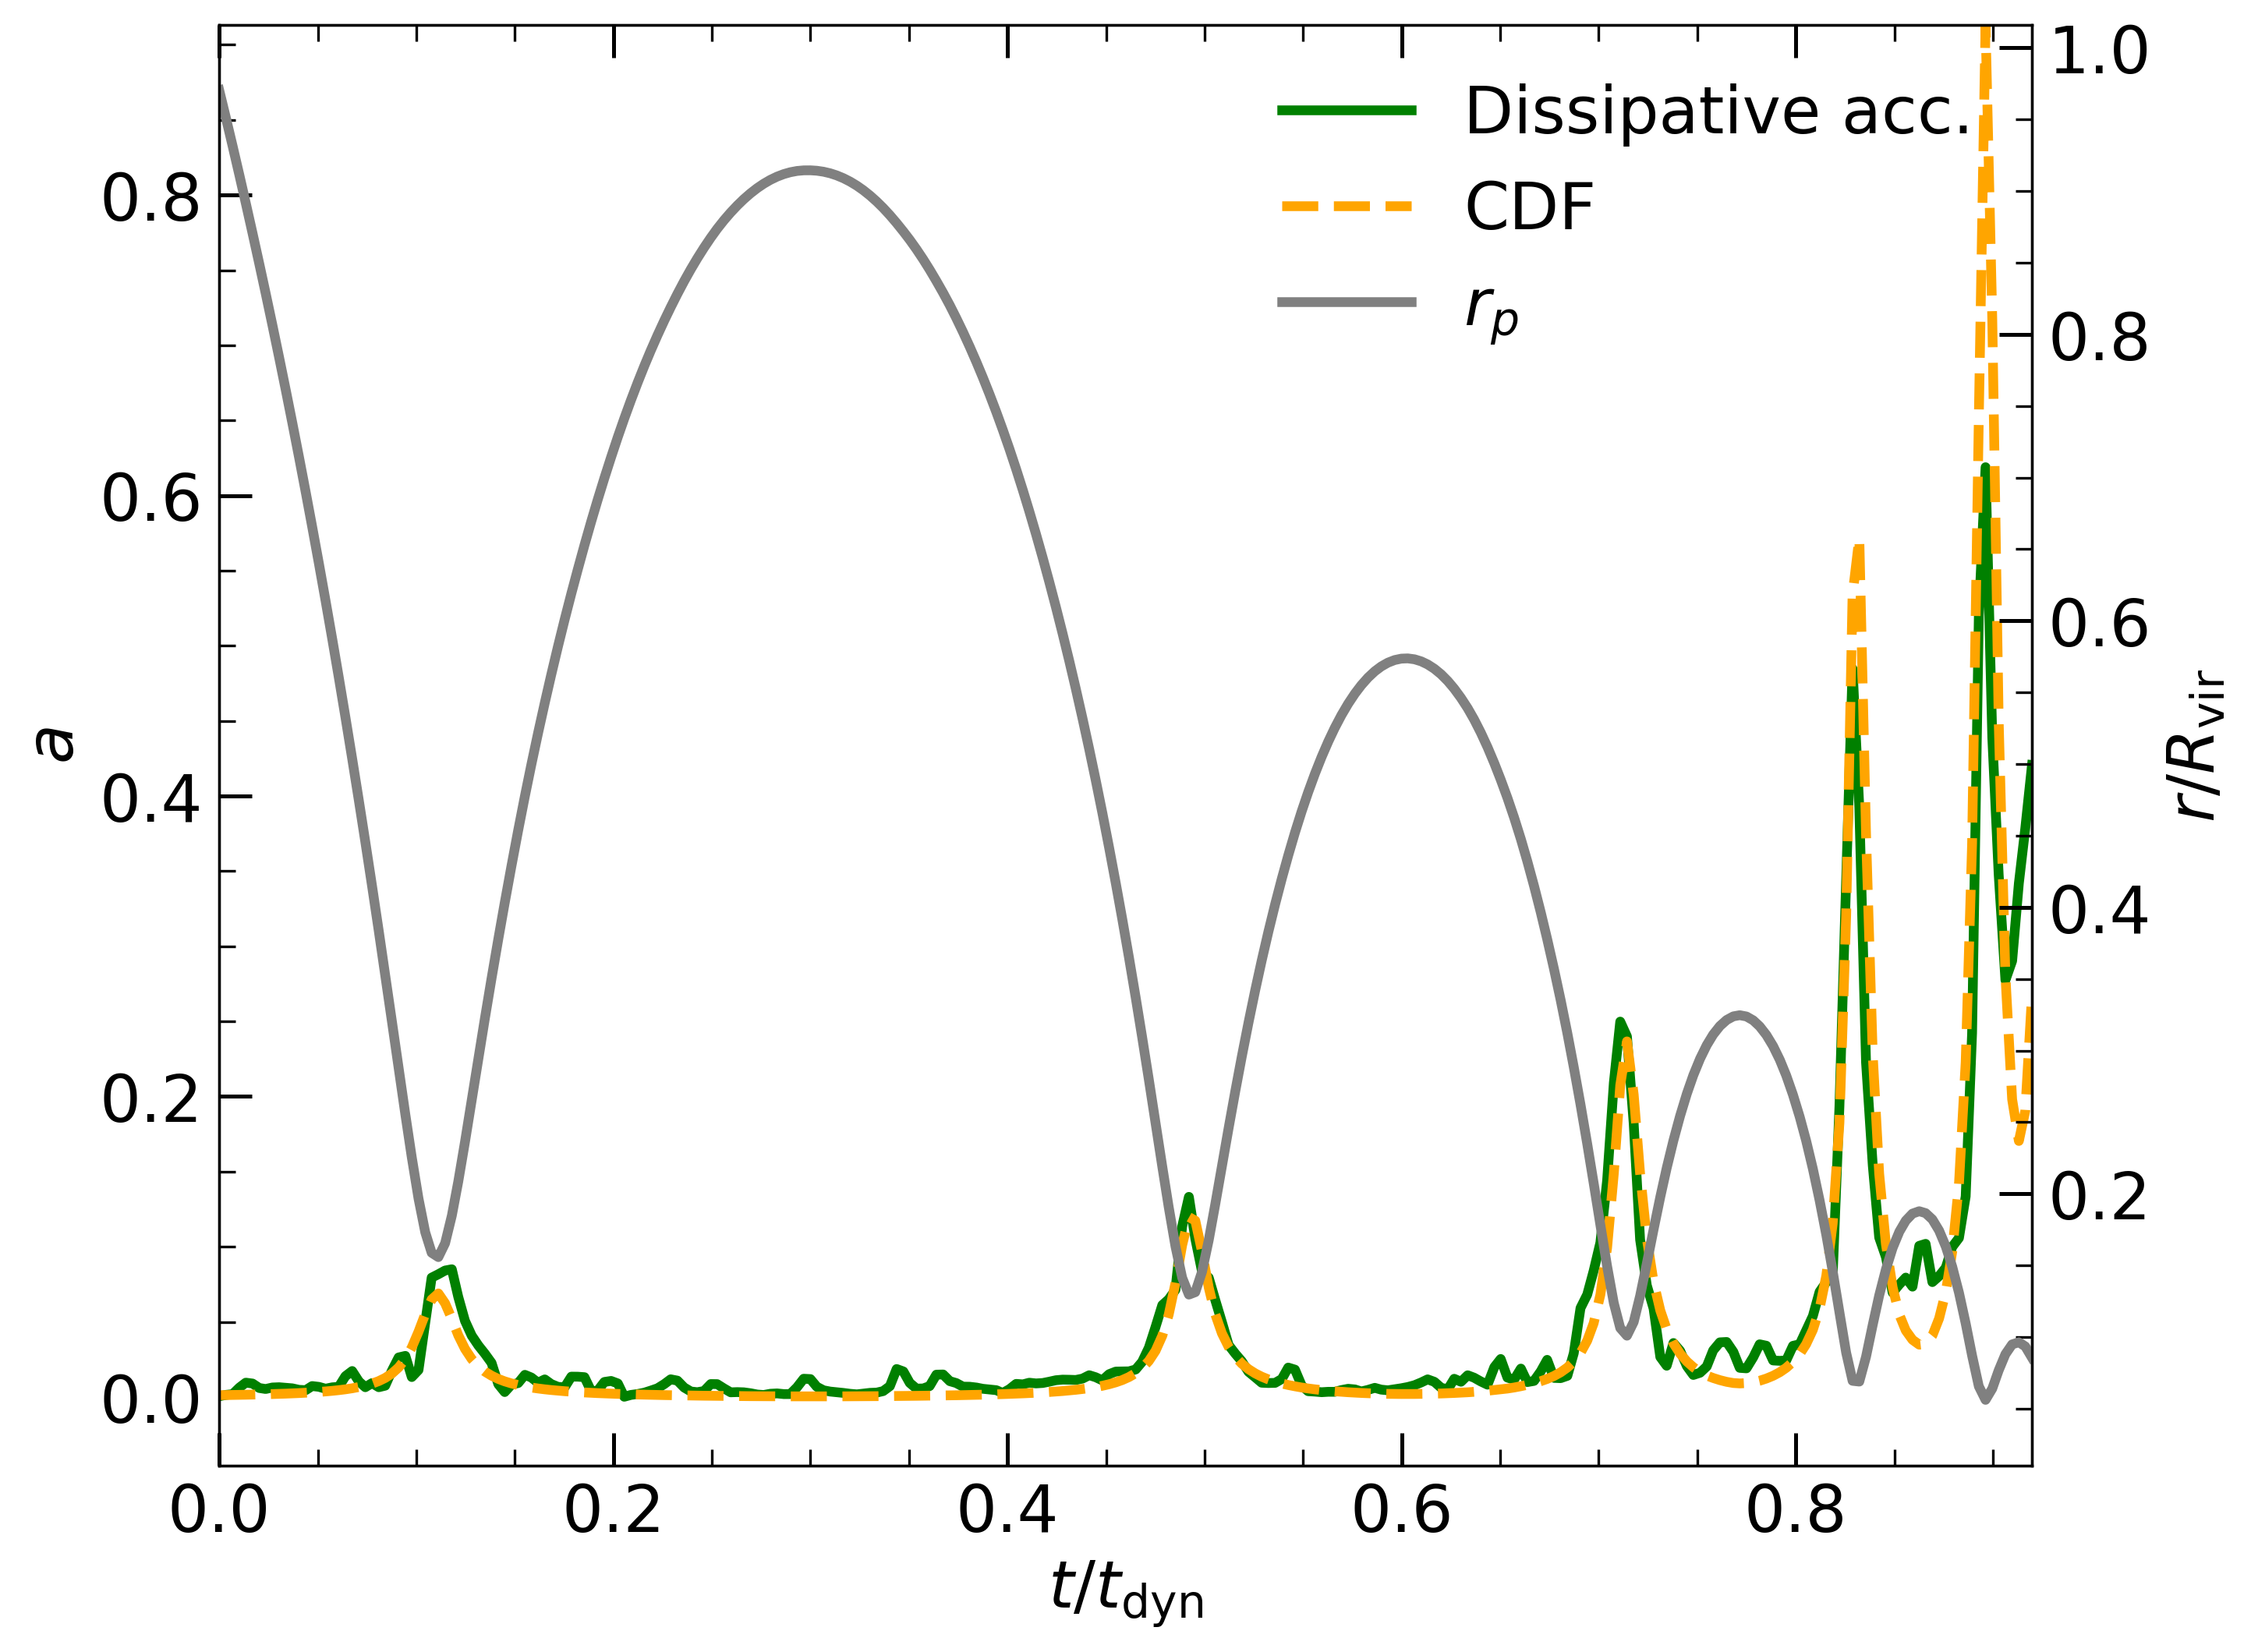
\includegraphics[width=\columnwidth]{images/pert_acc_cdf.png}
    \caption{Comparison of the magnitudes of \(\vb{a}_\text{diss}\) and the \acrshort{cdf} acting on a \(M_\text{tot} / 50\) perturber. The gray line shows the distance from the center of mass.}
    \label{fig:pert_acc_cdf}
\end{figure}

Equation~\ref{eq:cdf} is able to qualitatively predict the strength of the drag force acting on the perturber, but its reliability decreases as the orbit shrinks. However, this type of comparison depends on the decomposition of the total acceleration and does not account for directional differences between the \acrshort{cdf} and the actual dissipative component.

A more direct way to evaluate the validity of the \acrshort{cdf} formula is to assess whether the torque it predicts at each snapshot can reproduce the subsequent value of the angular momentum. Operationally, at a given time \(t_i\), let \(\vb{a}_\text{DF}^{t_i}\) be the \acrshort{cdf} acceleration, and \(\vb{L}_p^{t_i} = \vb{r}_p^{t_i} \times \vb{v}_p^{t_i}\) the perturber’s specific angular momentum. Then, we define the torque:
\[
\vb{M}_p^{t_i} = \vb{r}_p^{t_i} \times \vb{a}_\text{DF}^{t_i},
\]
and test whether the angular momentum at the next time step satisfies:
\[
\vb{L}_p^{t_{i+1}} = \vb{L}_p^{t_i} + \vb{M}_p^{t_i} (t_{i+1} - t_i).
\]
The result of this reconstruction procedure is shown in Figure~\ref{fig:pert_l_cdf}.

\begin{figure}
    \centering
    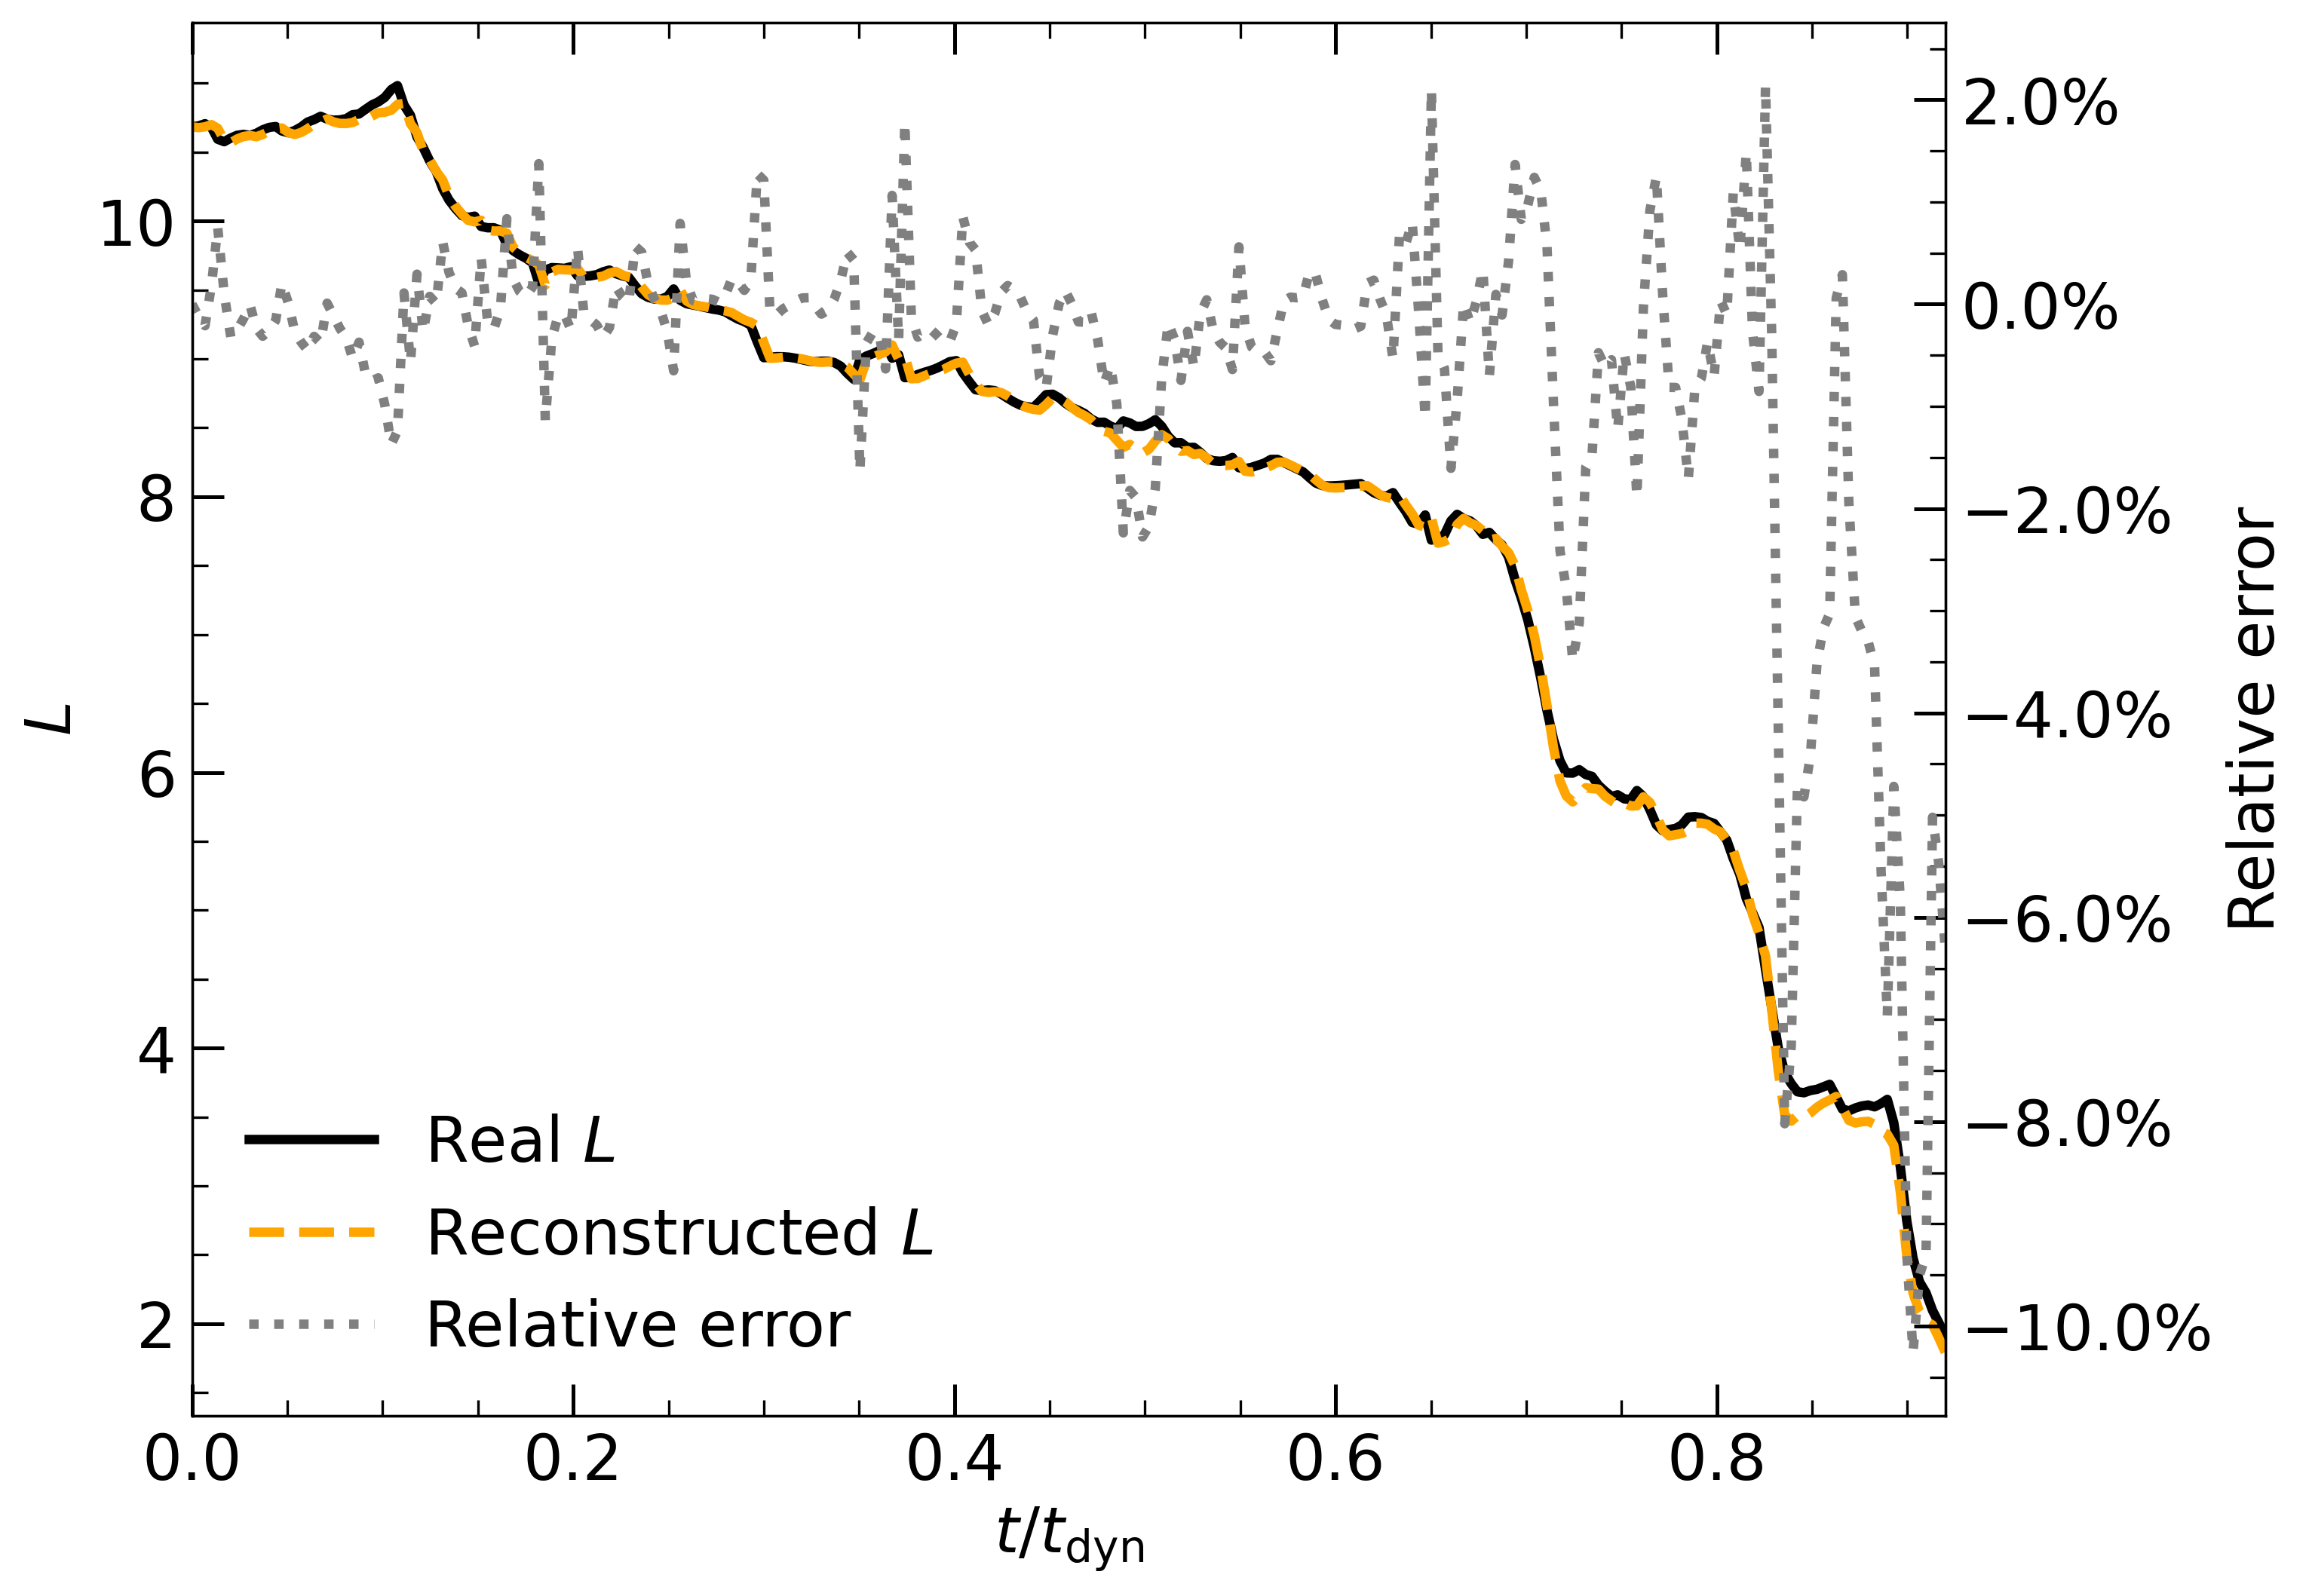
\includegraphics[width=\columnwidth]{images/pert_l_cdf.png}
    \caption{Reconstruction of the specific angular momentum evolution of a \(M_\text{tot} / 50\) perturber using the \acrshort{cdf}. The gray dotted line shows the relative percent error of the reconstructed \(L_p\) compared to the actual value.}
    \label{fig:pert_l_cdf}
\end{figure}

Although the \acrshort{cdf} is a first-order approximation, it is capable of predicting the orbital evolution of the perturber with a relative error of only a few percent for more than half of its lifetime. Beyond that point, the accuracy decreases rapidly.

\subsection{Circularity}

We now examine the evolution of the circularity \(\eta = L / L_\text{circ}(E)\) of the perturber’s orbit, computed using Eq.~\ref{eq:l_circ}. As shown in Figure~\ref{fig:pert_l_circ}, the circularity tends to increase over time.

\begin{figure}
    \centering
    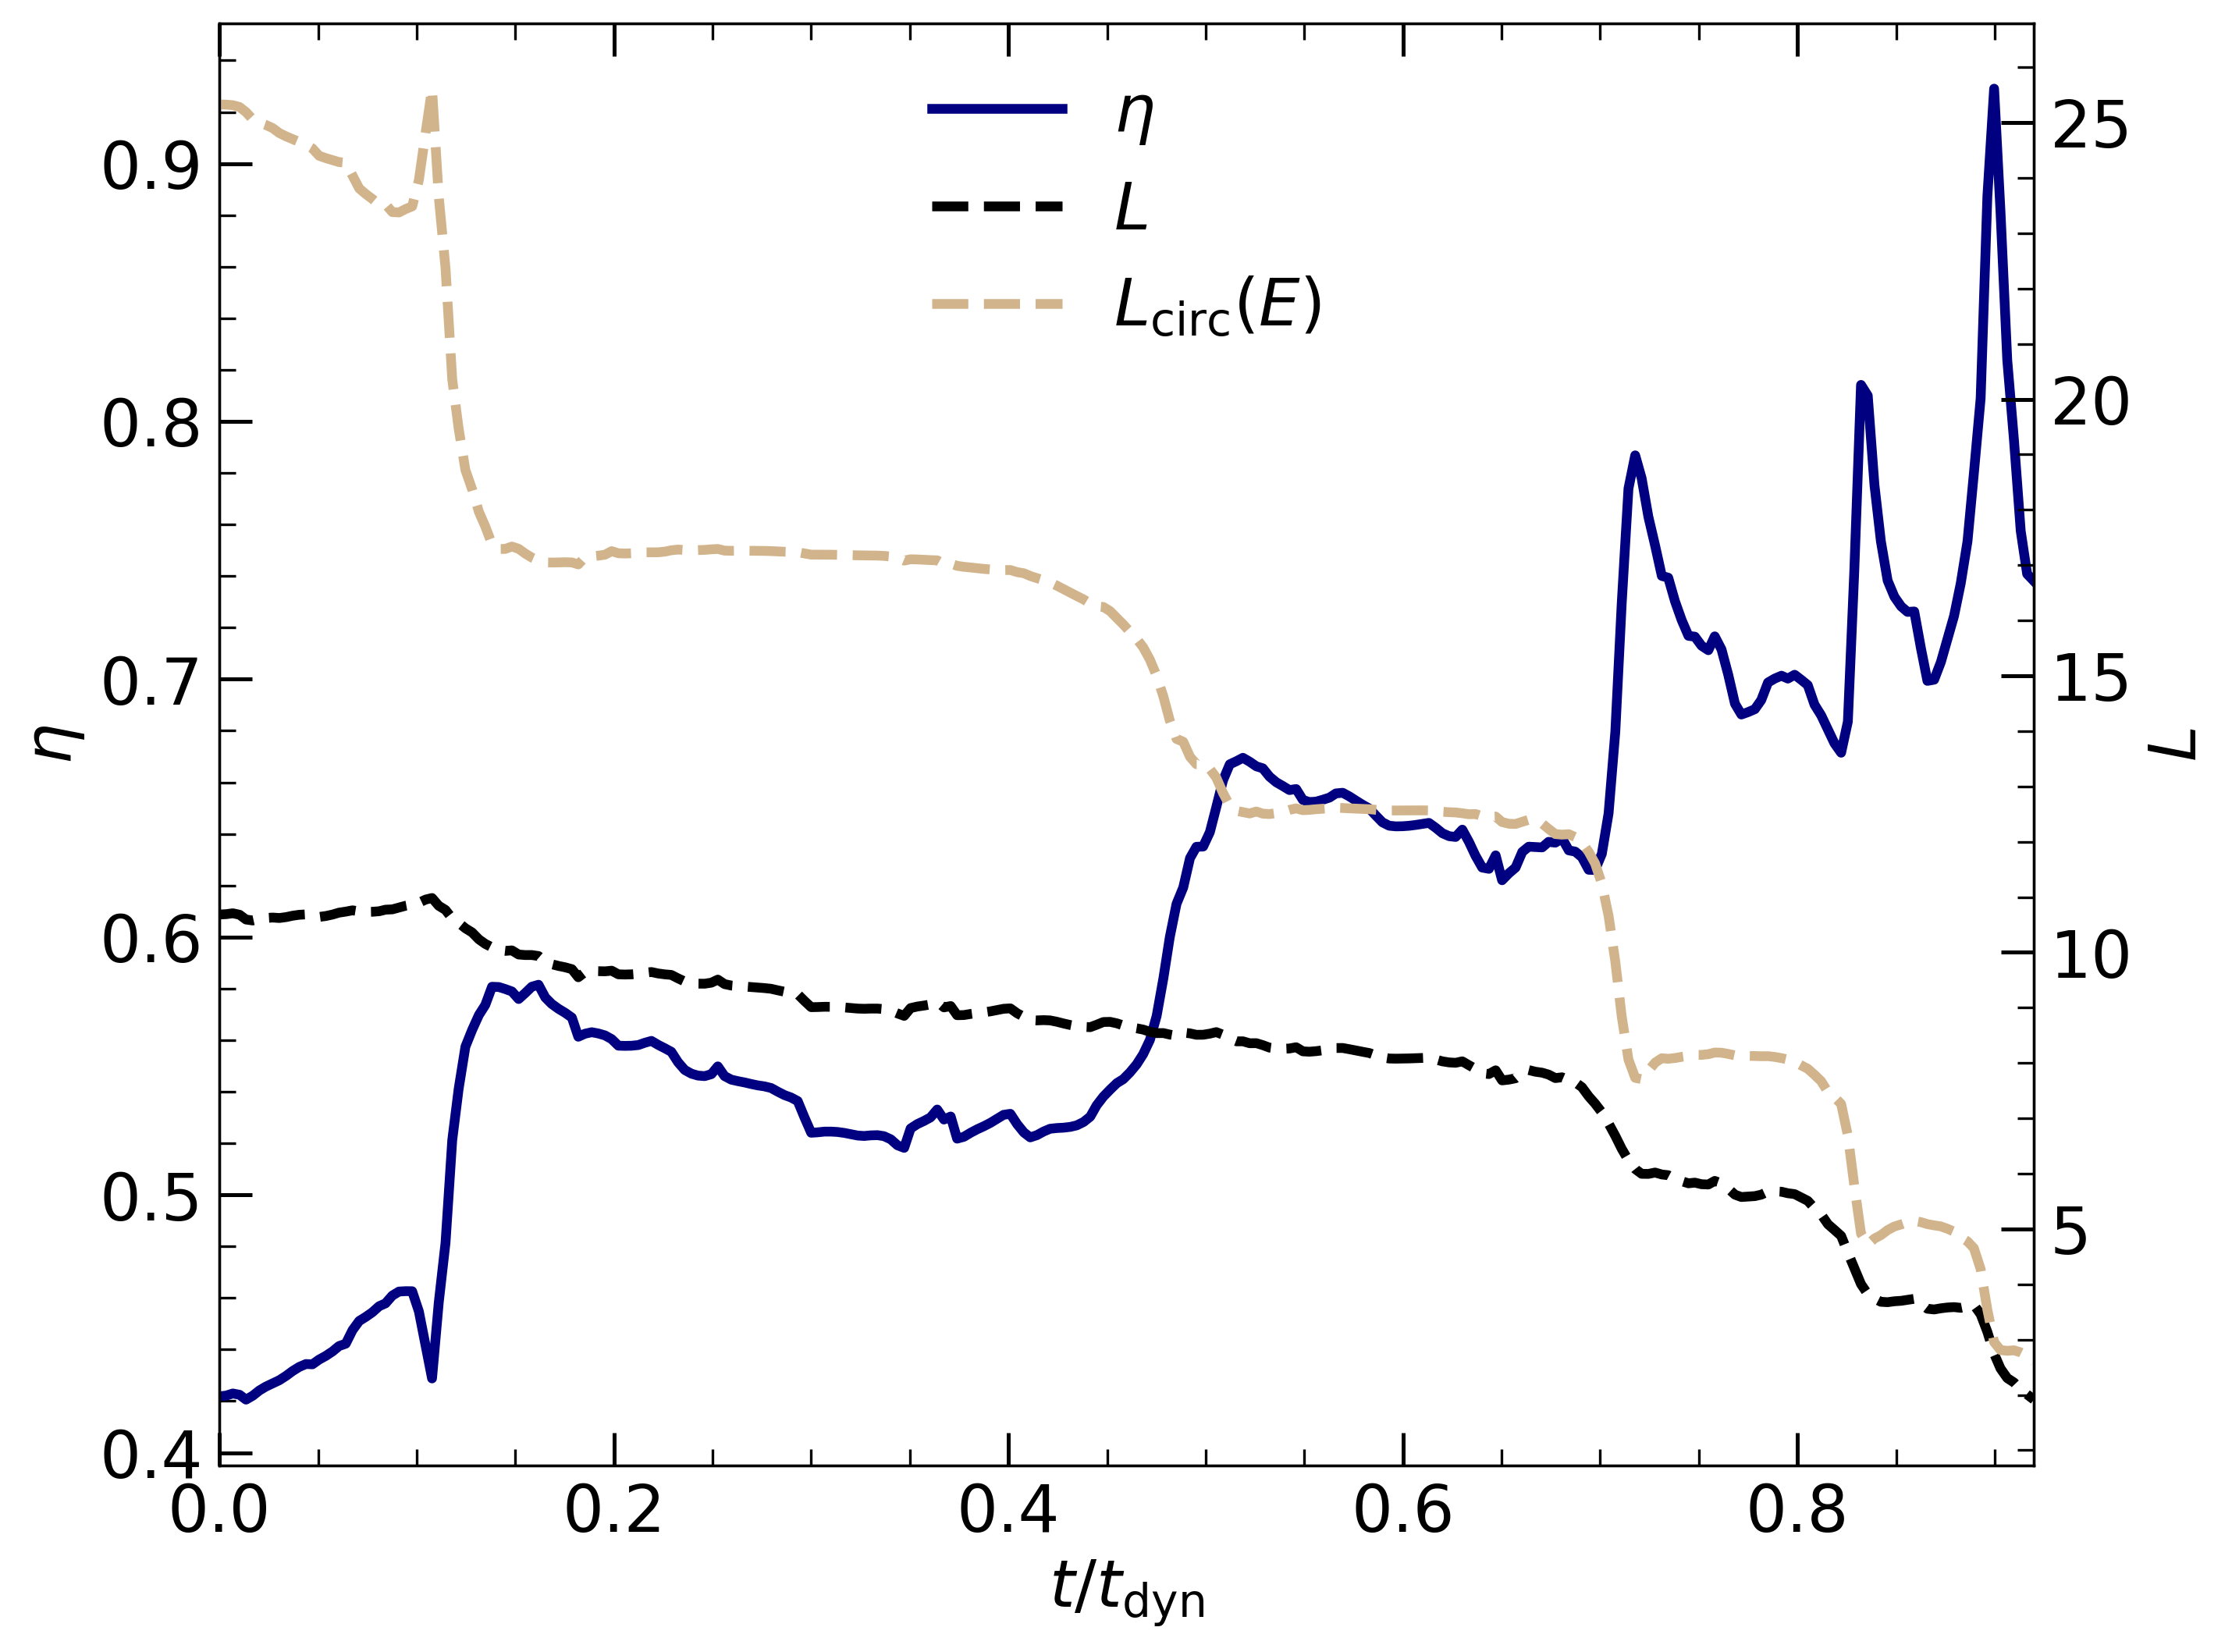
\includegraphics[width=\columnwidth]{images/pert_l_circ.png}
    \caption{Evolution of the circularity \(\eta = L / L_\text{circ}(E)\) of a \(M_\text{tot} / 50\) perturber initialized on a highly eccentric orbit. The dashed lines represent the specific angular momentum \(L\) and the corresponding circular angular momentum \(L_\text{circ}(E)\).}
    \label{fig:pert_l_circ}
\end{figure}

A similar trend is observed in other simulations, shown in Figure~\ref{fig:pert_eta_comp}, where the perturber was initialized at the virial radius with varying velocities and eccentricities. In all cases, the circularity increases progressively over time, approaching a maximum value of \(\eta \sim 1\) by the time the angular momentum reaches the threshold value \(L_\text{thr}\) (as defined in Fig.~\ref{fig:pert_dist_l}).

\begin{figure}
    \centering
    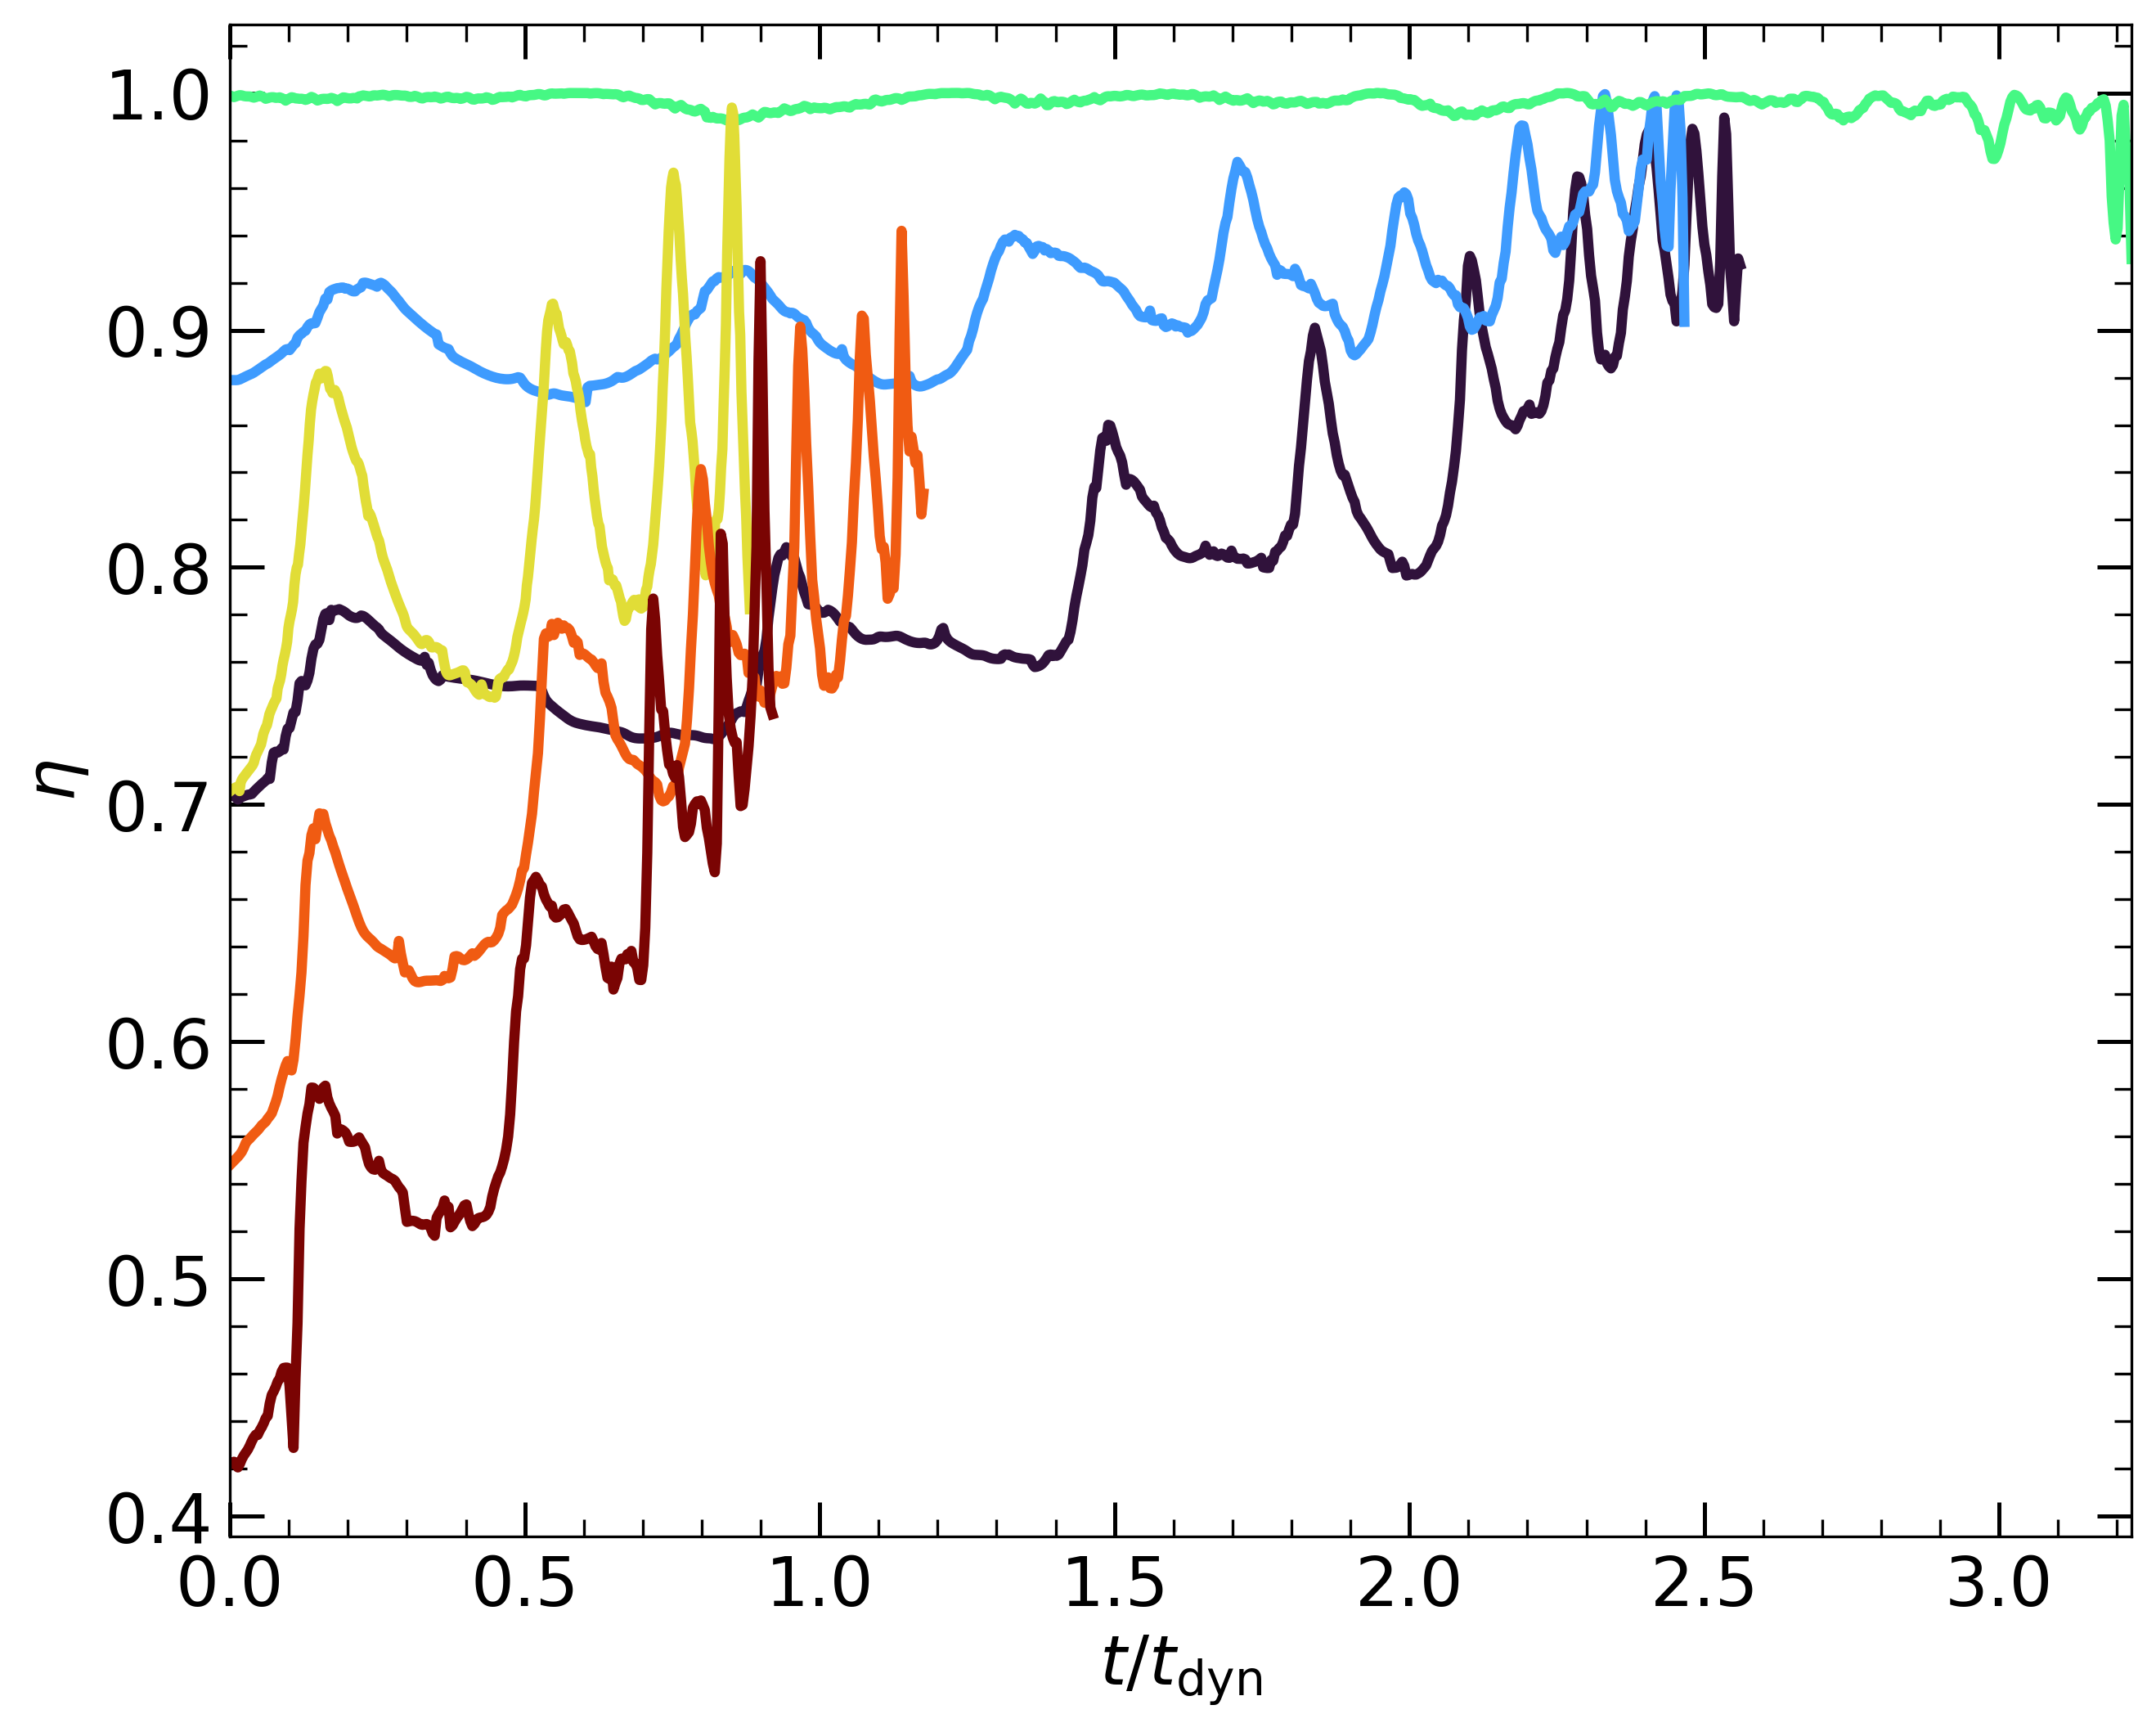
\includegraphics[width=\columnwidth]{images/eta_comparison.png}
    \caption{Comparison of the circularity evolution \(\eta\) for different simulations. All perturbers were initialized at the virial radius with varying orbital parameters.}
    \label{fig:pert_eta_comp}
\end{figure}

\section{Discussion}

The results presented in this work demonstrate that the \acrshort{cdf} formula can provide a good approximation of the instantaneous dissipative force acting on a perturber moving through a host distribution. The accuracy of the \acrshort{cdf} prediction is better assessed by comparing the torque it produces with the actual torque acting on the perturber, rather than by directly comparing the magnitudes of the forces. This is due to the decomposition of the total acceleration into radial and dissipative components, and to the fact that the system’s center of mass, while a good approximation, does not exactly coincide with the center of density of the distribution.

The \acrshort{cdf} formula reproduces the perturber’s angular momentum with a relative error of only a few percent for more than half of its lifetime. Beyond this point, the accuracy drops rapidly. The primary source of error as the perturber approaches the center of the distribution is likely the increasing inhomogeneity of the density profile, which leads to a more complex drag force not fully captured by the \acrshort{cdf} expression. Furthermore, the Coulomb logarithm in Eq.~\ref{eq:cdf} behaves almost like a free parameter, which can introduce significant uncertainty in high-density regions. In particular, the inclusion of the \(r_p / R_\text{vir}\) factor in the definition of \(b_\text{min}\) (see Section~\ref{sec:cdf_circularity_comp}), introduced to account for the increasing strength of interactions near the center, is not derived from first principles. A more physically motivated treatment of the Coulomb logarithm could enhance the predictive power of the \acrshort{cdf} formula.

In all simulations performed, the circularity of the perturber’s orbit steadily increases over time. According to \citeauthor{Vasiliev2022}, such behavior is expected for density profiles with inner slopes of \(\gamma = 3\). In our case, the adopted density profile displays a slope of \(\gamma \sim 3\) in the range \(R_\text{s} < r < R_\text{vir}\), and \(\gamma = 1\) for \(r \ll R_\text{s}\) (see Fig.~\ref{fig:density_comp}). This supports the observed trend toward circularization.

\begin{figure}
    \centering
    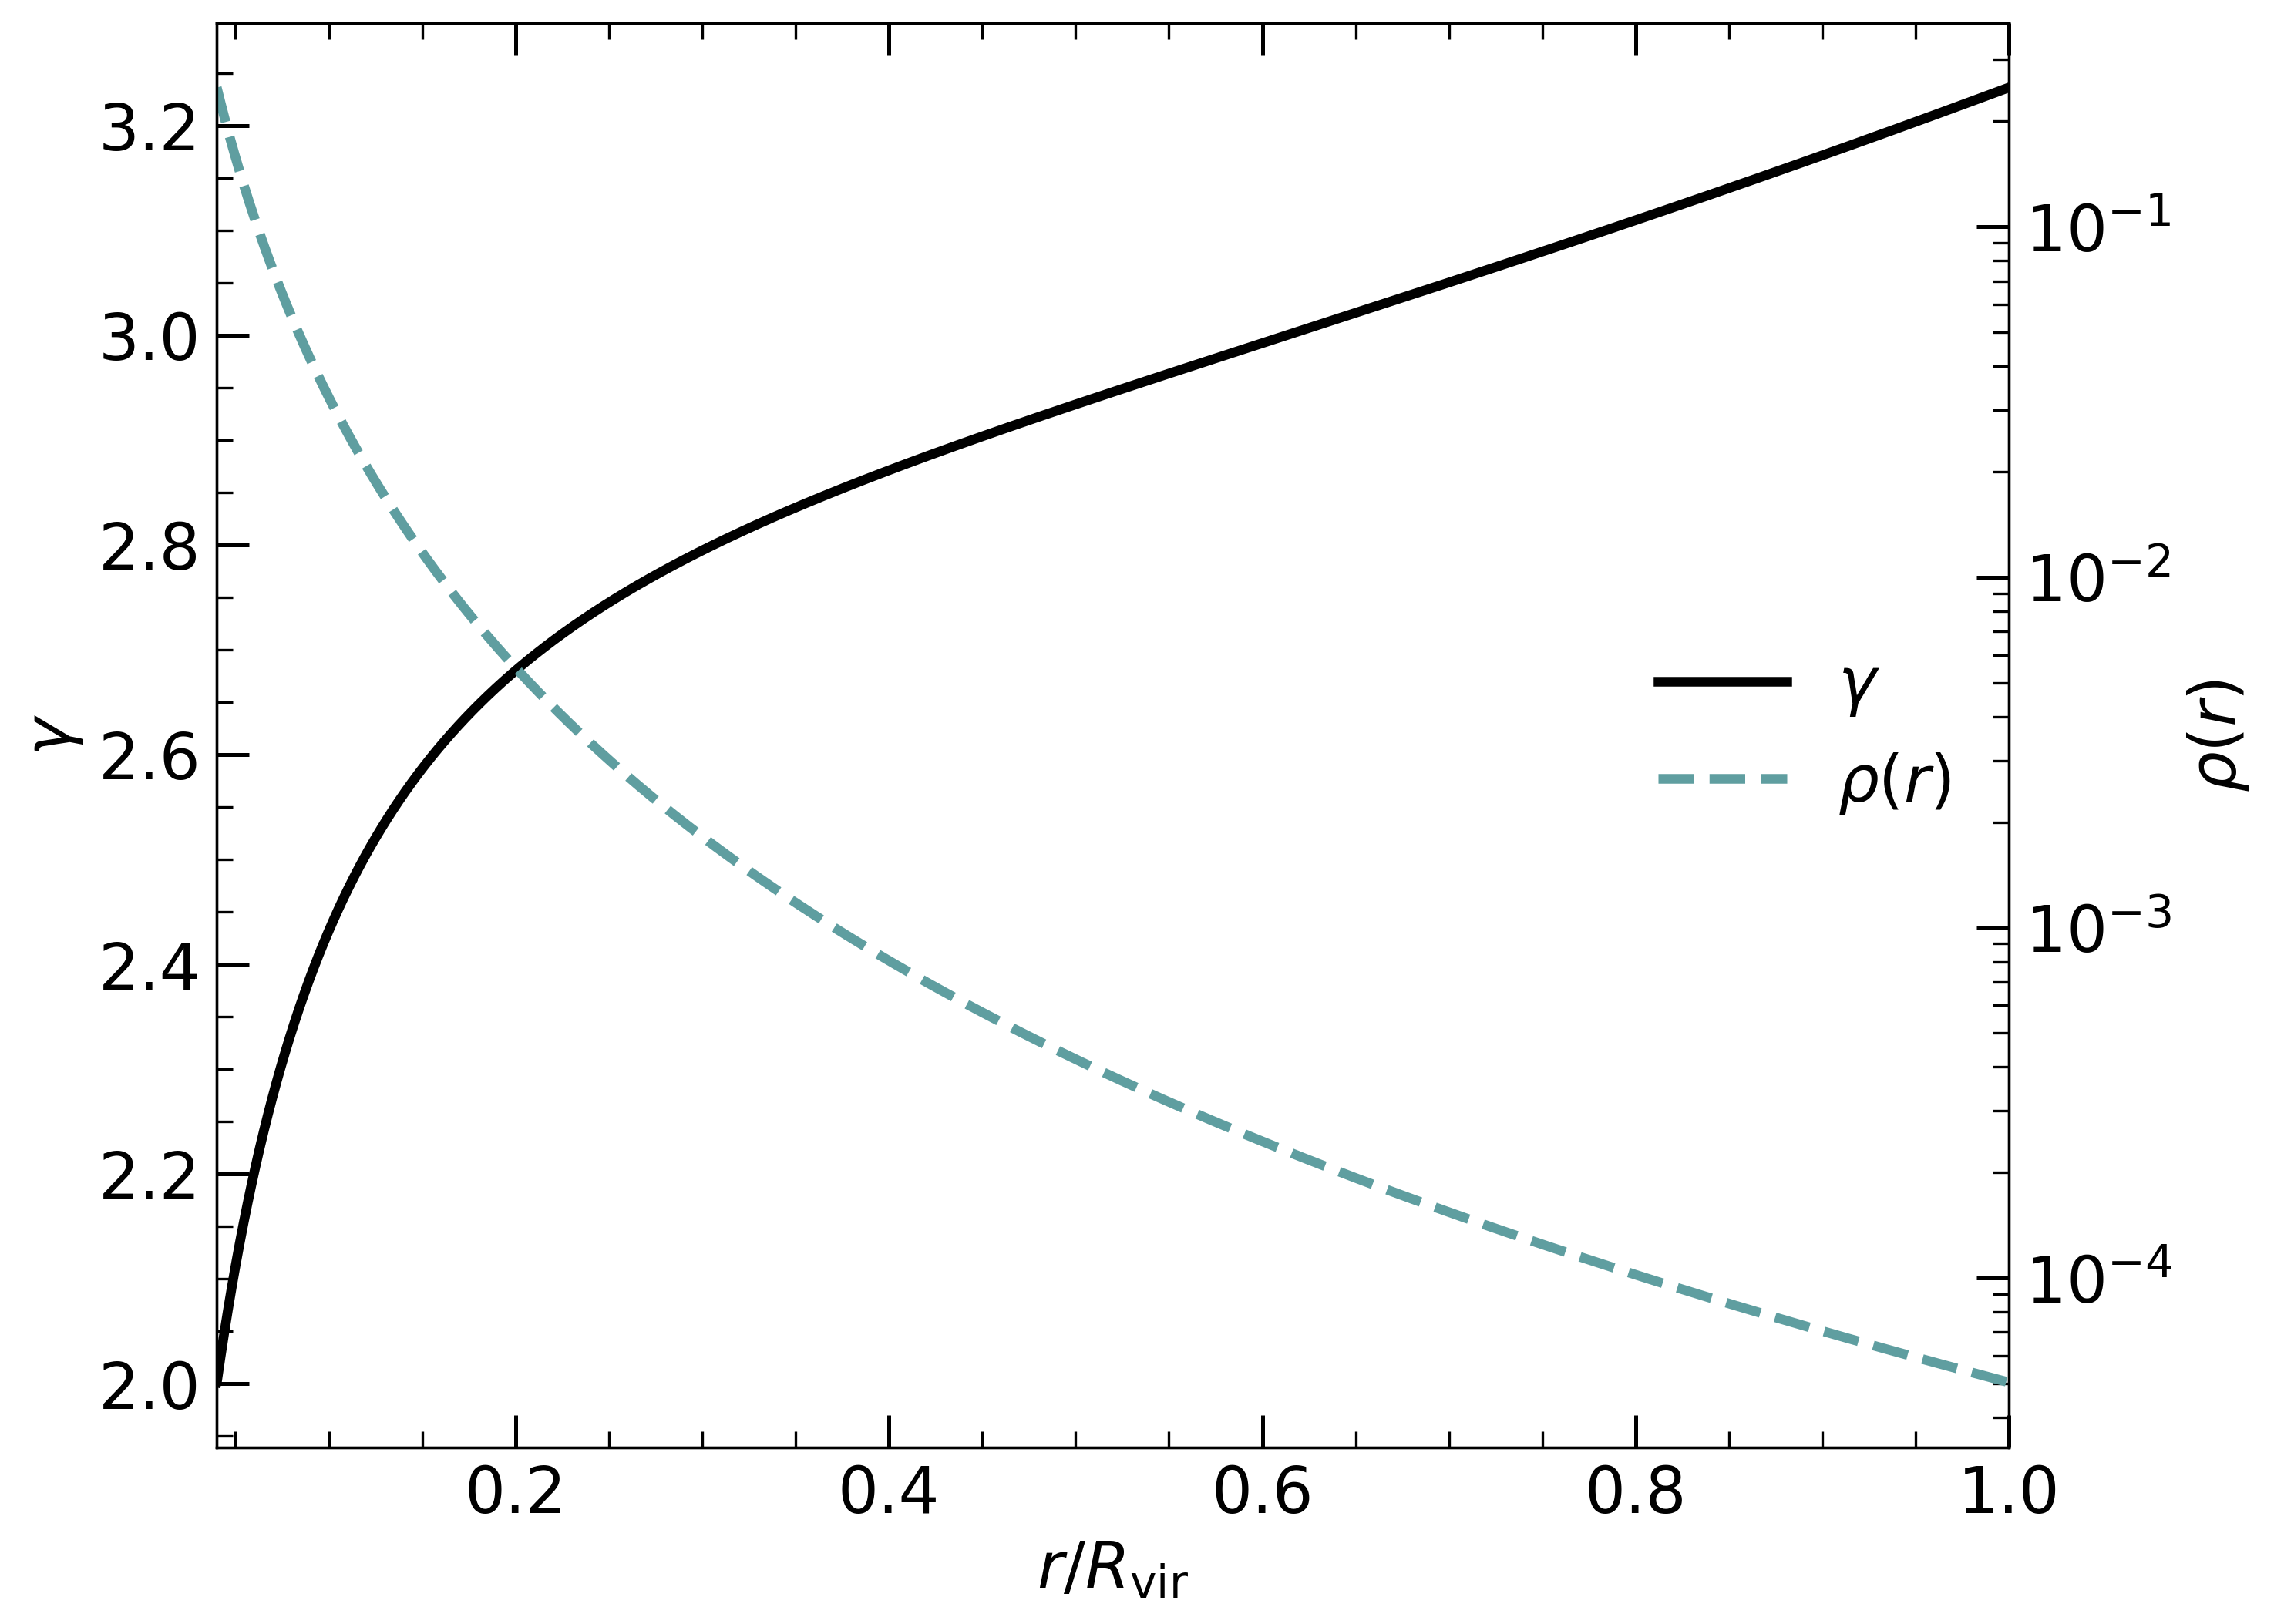
\includegraphics[width=\columnwidth]{images/rho_gamma.png}
    \caption{Slope \(\gamma\) of the density profile as a function of radius, computed as \(\gamma = -\dv{\log(\rho)}{\log(r)}\).}
    \label{fig:rho_gamma}
\end{figure}

The rate at which circularity increases depends on the initial conditions of the perturber. In particular, the more radial the initial orbit, the more rapid the circularization. According to \citeauthor{Vasiliev2022}, this effect is also enhanced for smaller mass ratios between the perturber and the host. However, since the slope of the density profile transitions from \(\gamma \sim 3\) near the virial radius \(R_\text{vir}\) to \(\gamma \sim 2\) closer to the scale radius \(R_\text{s}\) (see Fig.~\ref{fig:rho_gamma}), including the effect of satellite mass loss—as done by \citeauthor{Vasiliev2022}—could lead to a more complex evolution of the perturber’s circularity.

The role of numerical parameters, such as the softening length and integration time step, has not been systematically explored in this work. However, their influence could be non-negligible, particularly in the later stages of the inspiral where accelerations become stronger and orbital timescales shorten.

\section{Conclusion}

The \acrlong{cdf} formula, when applied to spherically symmetric collisionless systems, is capable of predicting the orbital evolution of a satellite moving through a host distribution. However, the accuracy of this prediction decreases as the perturber approaches higher-density regions. In particular, the choice of the Coulomb logarithm significantly affects the results, and a tailored, case-by-case treatment is recommended.

In the suppressed \acrlong{nfw} profile adopted in this work, the circularity of the perturber's orbit consistently increases over time, regardless of the initial orbital parameters. While this behavior is expected for steep density profiles, the inclusion of additional physical effects—such as satellite mass loss—could lead to a more intricate evolution of the orbital circularity, especially in the innermost regions of the distribution.

The results obtained using the simplified numerical setup presented in this work qualitatively agree with those of \citeauthor{Vasiliev2022} regarding the circularization of orbits in steep host distributions. However, they differ concerning the evolution of angular momentum as predicted by the \acrshort{cdf} formula. The \acrshort{cdf} may serve as a reasonable first-order approximation in idealized scenarios, but should be applied with caution when modeling more realistic systems.

\bibliographystyle{abbrvnat}
\bibliography{bibfile}

\end{document}
